%Version 2.1 April 2023
% See section 11 of the User Manual for version history
%
%%%%%%%%%%%%%%%%%%%%%%%%%%%%%%%%%%%%%%%%%%%%%%%%%%%%%%%%%%%%%%%%%%%%%%
%%                                                                 %%
%% Please do not use \input{...} to include other tex files.       %%
%% Submit your LaTeX manuscript as one .tex document.              %%
%%                                                                 %%
%% All additional figures and files should be attached             %%
%% separately and not embedded in the \TeX\ document itself.       %%
%%                                                                 %%
%%%%%%%%%%%%%%%%%%%%%%%%%%%%%%%%%%%%%%%%%%%%%%%%%%%%%%%%%%%%%%%%%%%%%

%%\documentclass[referee,sn-basic]{sn-jnl}% referee option is meant for double line spacing

%%=======================================================%%
%% to print line numbers in the margin use lineno option %%
%%=======================================================%%

%\documentclass[lineno,sn-basic]{sn-jnl}% Basic Springer Nature Reference Style/Chemistry Reference Style

%%======================================================%%
%% to compile with pdflatex/xelatex use pdflatex option %%
%%======================================================%%

%\documentclass[pdflatex,sn-basic]{sn-jnl}% Basic Springer Nature Reference Style/Chemistry Reference Style


%%Note: the following reference styles support Namedate and Numbered referencing. By default the style follows the most common style. To switch between the options you can add or remove “Numbered” in the optional parenthesis. 
%%The option is available for: sn-basic.bst, sn-vancouver.bst, sn-chicago.bst, sn-mathphys.bst. %  
 
%%\documentclass[sn-nature]{sn-jnl}% Style for submissions to Nature Portfolio journals

\documentclass[sn-basic]{sn-jnl}% Basic Springer Nature Reference Style/Chemistry Reference Style

%%$\documentclass[sn-mathphys,Numbered]{sn-jnl}% Math and Physical Sciences Reference Style

%%\documentclass[sn-aps]{sn-jnl}% American Physical Society (APS) Reference Style

%%\documentclass[sn-vancouver,Numbered]{sn-jnl}% Vancouver Reference Style

%%\documentclass[sn-apa]{sn-jnl}% APA Reference Style 
%%\documentclass[sn-chicago]{sn-jnl}% Chicago-based Humanities Reference Style
%%\documentclass[default]{sn-jnl}% Default
%%\documentclass[default,iicol]{sn-jnl}% Default with double column layout

%%%% Standard Packages
%%<additional latex packages if required can be included here>

\usepackage{graphicx}%
\usepackage{multirow}%
\usepackage{tabularx}
\usepackage{amsmath,amssymb,amsfonts}%
\usepackage{amsthm}%
\usepackage{mathrsfs}%
\usepackage[title]{appendix}%
\usepackage{xcolor}%
\usepackage{textcomp}%
\usepackage{manyfoot}%
\usepackage{booktabs}%
\usepackage{algorithm}%
\usepackage{algorithmicx}%
\usepackage{algpseudocode}%
\usepackage{listings}%
\usepackage{bm}

%%%%
%%% Added packages
\usepackage{multirow} %for multirowtables
\usepackage{longtable} %for long table



%%%%%=============================================================================%%%%
%%%%  Remarks: This template is provided to aid authors with the preparation
%%%%  of original research articles intended for submission to journals published 
%%%%  by Springer Nature. The guidance has been prepared in partnership with 
%%%%  production teams to conform to Springer Nature technical requirements. 
%%%%  Editorial and presentation requirements differ among journal portfolios and 
%%%%  research disciplines. You may find sections in this template are irrelevant 
%%%%  to your work and are empowered to omit any such section if allowed by the 
%%%%  journal you intend to submit to. The submission guidelines and policies 
%%%%  of the journal take precedence. A detailed User Manual is available in the 
%%%%  template package for technical guidance.
%%%%%=============================================================================%%%%

%\jyear{2021}%

%% as per the requirement new theorem styles can be included as shown below
%\theoremstyle{thmstyleone}%
%\newtheorem{theorem}{Theorem}%  meant for continuous numbers
%%\newtheorem{theorem}{Theorem}[section]% meant for sectionwise numbers
%% optional argument [theorem] produces theorem numbering sequence instead of independent numbers for Proposition
%\newtheorem{proposition}[theorem]{Proposition}% 
%%\newtheorem{proposition}{Proposition}% to get separate numbers for theorem and proposition etc.

%\theoremstyle{thmstyletwo}%
%\newtheorem{example}{Example}%
%\newtheorem{remark}{Remark}%

%\theoremstyle{thmstylethree}%
%\newtheorem{definition}{Definition}%

%\raggedbottom
%%\unnumbered% uncomment this for unnumbered level heads

\begin{document}

%\title[Article Title]{Are we ready to track internally displaced persons from outer space? Insights from the Russia-Ukraine War}
\title[Article Title]{Estimation of Internal Displacement in Ukraine from Satellite-Based Car Detections}

%%=============================================================%%
%% Prefix	-> \pfx{Dr}
%% GivenName	-> \fnm{Joergen W.}
%% Particle	-> \spfx{van der} -> surname prefix
%% FamilyName	-> \sur{Ploeg}
%% Suffix	-> \sfx{IV}
%% NatureName	-> \tanm{Poet Laureate} -> Title after name
%% Degrees	-> \dgr{MSc, PhD}
%% \author*[1,2]{\pfx{Dr} \fnm{Joergen W.} \spfx{van der} \sur{Ploeg} \sfx{IV} \tanm{Poet Laureate} 
%%                 \dgr{MSc, PhD}}\email{iauthor@gmail.com}
%%=============================================================%%

\author*[1]{\fnm{Marie-Christine} \sur{Rufener}}\email{macrufener@gmail.com}
\author[1]{\fnm{Ferda} \sur{Ofli}}\email{fofli@hbku.edu.qa}
\author[1]{\fnm{Masoomali} \sur{Fathekia}}\email{mfatehkia@hbku.edu.qa}
\author*[2]{\fnm{Ingmar} \sur{Weber}}\email{iweber@cs.uni-saarland.de}
%\equalcont{These authors contributed equally to this work.}


%\affil[1]{\orgdiv{Department}, \orgname{Organization}, \orgaddress{\street{Street}, \city{City}, \postcode{610101}, \state{State}, \country{Country}}}

\affil*[1]{\orgdiv{Qatar Computing Research Institute}, \orgname{Hamad Bin Khalifa University}, \orgaddress{\city{Doha}, \country{Qatar}}}

\affil*[2]{\orgdiv{Computer Science Department}, \orgname{Saarland University}, \orgaddress{\city{Saarbrücken}, \country{Germany}}}


%%==================================%%
%% sample for unstructured abstract %%
%%==================================%%

\abstract{
Armed conflicts such as the Russia-Ukraine war force millions of people to flee from their homes, with many seeking refuge within the borders of their country. Estimating the numbers and whereabouts of internally displaced people (IDP) is therefore paramount to providing targeted humanitarian assistance. Unfortunately, especially in a conflict or disaster setting, on-the-ground data collection is often inadequate to provide accurate and timely information. In contrast, non-traditional data sources such as satellite imagery offer the possibility to sidestep some of the challenges and help to improve our understanding of the dynamics of IDPs, and hence, provide better assistance. 
Our motivating question was to evaluate whether internal displacement patterns can be estimated from the spatial-temporal changes in the car counts obtained from multi-temporal satellite imagery. To do so, we collected over 1000 very-high-resolution images for the main urban areas in Ukraine over the period 2019-2022. To these satellite images, we subsequently applied a state-of-the-art computer vision model to detect and count cars. These were then linked to gridded population data in order to predict internal displacements through either a ratio or non-linear model. Our findings suggest a clear East-to-West movement of cars in the first months following the start of the war (24 February 2022). Data sparsity nevertheless prevented any fine-grained evaluation, which propagated to the level of the IDP prediction. For most of the applicable cities, we could distinguish a clear positive and non-linear trend between the number of people and cars. This allowed us to predict, to some extent, the sub-national people dynamics during the War and also suggested an East-to-West movement. While we present a resource-saving and innovative approach to estimate IDPs, it should be acknowledged that satellite imagery and current computer vision models present some shortcomings that could mask detailed IDPs dynamics. We end this article by discussing these aspects in more detail and by outlining opportunities for future research.}

%%================================%%
%% Sample for structured abstract %%
%%================================%%

% \abstract{\textbf{Purpose:} The abstract serves both as a general introduction to the topic and as a brief, non-technical summary of the main results and their implications. The abstract must not include subheadings (unless expressly permitted in the journal's Instructions to Authors), equations or citations. As a guide the abstract should not exceed 200 words. Most journals do not set a hard limit however authors are advised to check the author instructions for the journal they are submitting to.
% 
% \textbf{Methods:} The abstract serves both as a general introduction to the topic and as a brief, non-technical summary of the main results and their implications. The abstract must not include subheadings (unless expressly permitted in the journal's Instructions to Authors), equations or citations. As a guide the abstract should not exceed 200 words. Most journals do not set a hard limit however authors are advised to check the author instructions for the journal they are submitting to.
% 
% \textbf{Results:} The abstract serves both as a general introduction to the topic and as a brief, non-technical summary of the main results and their implications. The abstract must not include subheadings (unless expressly permitted in the journal's Instructions to Authors), equations or citations. As a guide the abstract should not exceed 200 words. Most journals do not set a hard limit hhttps://www.overleaf.com/project/646c7a7f50d0ef6c36e9fd85owever authors are advised to check the author instructions for the journal they are submitting to.
% 
% \textbf{Conclusion:} The abstract serves both as a general introduction to the topic and as a brief, non-technical summary of the main results and their implications. The abstract must not include subheadings (unless expressly permitted in the journal's Instructions to Authors), equations or citations. As a guide the abstract should not exceed 200 words. Most journals do not set a hard limit however authors are advised to check the author instructions for the journal they are submitting to.}

\keywords{Car Detection, Remote Sensing, Satellite Imagery, Convolutional Neural Network,  Crisis Response, Internal Displacement, Migration, Societal Computing}

%%\pacs[JEL Classification]{D8, H51}

%%\pacs[MSC Classification]{35A01, 65L10, 65L12, 65L20, 65L70}

\maketitle

%%%%%%%%%%%%%%%%%%%%%%%%%%%%%%%%%%%%%%%%%%%%%%%


%%%%%%%%%%%%%%%%%%%%%%%%%%%%%%%%%%%%%%%
%%%%%%        Introduction       %%%%%% 
%%%%%%%%%%%%%%%%%%%%%%%%%%%%%%%%%%%%%%%
\section{Main}\label{Introduction}
%\textbf{\textcolor{blue}{Ingmar: Check if the template allows a motivating figure. Having a motivation figure, e.g. showing before/after satellite imagery with some cars identified, would serve as a good motivation.}}
%\textbf{\textcolor{orange}{Marie: Yes - Done!}}

Millions of civilians are uprooted each year from their places of residence due to conflicts, human rights violations, and natural disasters \citep{UNHCR_2022}. The number of forcibly displaced people has more than doubled over the past decade, reaching a record high of 100 million in 2022 \citep{UNHCR_2022_news}. Internally displaced people (IDPs), i.e., people forced to leave their homes but who remain within their country's border, accounted for more than 70\% of the recorded movements, marking a 20\% increase compared to the previous year \citep{IDMC_2023}. According to the latest report of the Internal Displacement Monitoring Centre (iDMC), the escalating number of conflicts and violence in the past year pushed the figure to an unprecedented 28.3 million displacements worldwide \citep{IDMC_2023}. Such alarming numbers raise international concerns, as IDPs are amongst the most vulnerable people and often in need of humanitarian assistance to ensure their safety, as well as access to medical care, services, and food \citep{UNHCR_2022}. 

While there have been wide-ranging international efforts to measure the scale of \emph{cross-border} population flows, estimation of \emph{within-country} migration flows are particularly prone to inaccuracies, lack of timely updates, and lack of disaggregation, e.g., by age \citep{Checchi_et_al_2017, Ratnayake_et_al_2022}. This also applies in the context of the ongoing Russia-Ukraine War, which triggered the largest humanitarian crisis in Europe since World War II. As of December 2023, over 28 million border crossings from Ukraine have been registered since the start of the war (24 February 2022), in addition to 6 million Ukrainians who sought refuge in neighboring countries and another 5 million within the borders of their country \citep{UNHCR_2023, IOM_2023}. The volatile situation of the conflict has resulted in pendular migration not only between Ukraine and adjacent countries but also within the country itself. Although public authorities have a good understanding of the population flow to and from receiving countries, less is known about the Ukrainians' displacement pattern at the sub-national level \citep{Rowe_et_al_2022}. 

To date, most information on IDPs is collected by humanitarian organizations through either phone- or field-based surveys \citep{Baal_et_al_2017, Leasure_et_al_2023}. In a conflict or disaster, however, these traditional data sources often fail to provide accurate and timely information, especially during the acute phase of the displacement crisis \citep{Baal_et_al_2017, Ratnayake_et_al_2022}. In armed conflicts, on-the-ground enumerators can be exposed to life-threatening risks, or have their access hindered by either infrastructural damages or inaccessibility to more remote areas \citep{Abdelmagid_Checchi_2018}. As a consequence, most countries rely on a patchwork of IDP estimates that arise from various independent assessments, each of which is collected for different purposes that ultimately yield conflicting IDP estimates \citep{Baal_et_al_2017}.

In light of such limitations, the use of non-traditional data for monitoring mobility patterns has gained momentum among both the scientific and the humanitarian community due to their untapped potential to sidestep some of the current data limitations \citep{Baal_et_al_2017, Quinn_et_al_2018, Weber_et_al_2021}. 
A large body of work has looked at the potential use of anonymized call detail records (CDR) from mobile phone operators to monitor mobility patterns, in particular in the context of communicable diseases, and most recently during the COVID-19 pandemic \citep{Williams_et_al_2015, Wesolowski_et_al_2012, Wesolowski_et_al_2016, Oliver_et_al_2020}. 

While CDR data is undoubtedly useful, procuring access is a major hurdle, as are difficulties in quickly transferring a methodology from one country to another. 
To address these concerns, a growing body of literature has been exploring digital traces from social media platforms, which are more easily accessible and persistent across countries \citep[e.g.,][]{mazzolietal20plosone, Zagheni_et_al_2014, Palotti_et_al_2020, Rowe_et_al_2022, Leasure_et_al_2023}. Others, in turn, have been relying on satellite imagery to estimate population dynamics through either refugee settlement detection \citep{Quinn_et_al_2018} or analysis of nightlights data \citep{Witmer_et_al_2011, Coscieme_et_al_2017}.

Building upon these studies, we advocate that satellite imagery bears a fertile, and yet largely under-explored, ground for studying internal population displacements. News channels all around the world reported the fleeing of thousands of Ukrainians by means of personal or shared vehicles during the first weeks following the full-scale Russian invasion. Countless numbers of vehicles stretching dozens of kilometers have been recorded at the major checkpoints on the Western border, capturing the evasion of Ukrainians from the Eastern to the Western regions \citep[e.g.,][]{Burnett_et_al_2022, HRW_2022, Vasovic_Zinets_2022}. 

%\textcolor{green}{Somewhere cite Bircan and Emre Eren Korkmaz 2021 https://www.nature.com/articles/s41599-021-00910-x re ethical risks. Probably also Huub Dijstelbloem 2017 https://www.nature.com/articles/543032a -- Ingmar}
%\textcolor{orange}{I've tried to add a closing paragraph in the Discussion section to include these two papers. However, we might need some reworking there. - Marie}

This vehicle-facilitated displacement behavior raises the question of whether internal displacement patterns can be estimated from the spatial-temporal changes in car counts obtained from satellite imagery. To pursue this research question, we collected a total of 1009 very-high-resolution satellite images between 2019-2022, spanning 61 cities across Ukraine. Of these images, only 534 images remained for analysis after undergoing our data post-processing pipeline, with most cities remaining with less than 10 images throughout the time series (Fig.~\ref{figSM_Nimages}). Furthermore, the monthly data availability was generally sporadic for all cities, with several temporal gaps along the time series (i.e., months without any data) (Fig.~\ref{figSM_DatAvail}). However, data coverage was much better during the months succeeding the start of the war than during the pre-conflict period, especially for cities heavily involved in the conflict (e.g., Kharkiv, Donetsk, Mariupol, Odessa, and Ivano-Frankivsk; Fig.~\ref{figSM_DatAvail}). This likely reflects operational adjustments by the satellite operator in response to the demand for images from the conflict areas.


Despite the data shortages, visual inspection of these images revealed some clear pre-war vs. wartime patterns in the number of cars across multiple cities. For example, Mariupol, one of the most heavily affected cities by the war, suffered a massive drop in the number of cars during the first month succeeding the war when compared with the same month and region prior to the COVID-19 pandemic (Fig. \ref{fig_motivationfig}a,b). The opposite trend was observed for the city of Uzhhorod on the Slovakian border, with a substantial increase in the number of vehicles during the months succeeding the outbreak of the war when contrasted to the pre-war period (Fig. \ref{fig_motivationfig}c,d). 


These two examples illustrate the apparent connection between the number of cars and people, as the car dynamics seemingly follow the general East-West migration pattern that has been previously reported for Ukraine \citep{Rowe_et_al_2022, Leasure_et_al_2023}. On this basis, the current study proposes a \emph{novel methodology to estimate IDPs}, using the ongoing Russia-Ukraine War as a motivating case study. By using a computer vision model in combination with a robust statistical analysis, we modeled the population-car relationship for multiple cities and estimated the sub-national people displacement whenever applicable.




%%%%%%%%%%%%%%%%%%%%%%%%%%%%%%%%%%
%%%%%%        Results       %%%%%% 
%%%%%%%%%%%%%%%%%%%%%%%%%%%%%%%%%%
\section{Results}\label{Results}


%\subsection{Data overview}

%A total of 1009 very-high-resolution satellite images, with a ground sampling distance between 30cm and 50cm, provided by Maxar\footnote{\url{https://www.maxar.com/}} were collected and processed for the selected Ukrainian cities and time period, with the bulk of images taken between 8 AM and 9 AM UTC (Fig. ~\ref{figSM_Nimages_per_hour}). Of these, only 534 images remained after the data post-processing pipeline. A small number of cities had only a single image throughout the time series (Fig.~\ref{figSM_Nimages}) and were removed. In general, the monthly data availability was sporadic for all cities, with several temporal gaps along the time series (i.e., months without any data) (Fig.~\ref{figSM_DatAvail}). However, data coverage was much better during the months succeeding the start of the war than during the pre-conflict period, especially for cities heavily involved in the conflict (e.g., Kharkiv, Donetsk, Mariupol, Odessa, and Ivano-Frankivsk; Fig.~\ref{figSM_DatAvail}). 

%\subsection{CNN model overview}
%\textcolor{orange}{
%\begin{itemize}
%    \item Ferda, is there any relevant aspect of the CNN model that should be explored in the results? - Marie
%\end{itemize}
%}

In the following two sections, we first describe our more basic and measurement-centric analysis of (raw) car counts (Section~\ref{sec:car_dynamics}). Subsequently, we describe a more advanced and modeling-centric analysis that uses the changes in car counts to estimate changes in \emph{population} counts (Section~\ref{sec:pop_dynamics}).


\subsection{Spatio-temporal car dynamics}\label{sec:car_dynamics}

Evaluating the car dynamics on a monthly resolution was largely infeasible, given the temporal data gaps within each city (Fig.~\ref{figSM_DatAvail}). Nevertheless, trends in the car dynamics become more apparent at coarser temporal resolution and we therefore present the following results on a quarterly and yearly resolution to ease interpretation (Fig.~\ref{Fig_CarSpatDyn}).

At the quarter-of-year resolution, our results suggest an increasing and progressive trend of car displacement from East-to-West throughout the year (Fig. \ref{Fig_CarSpatDyn}a). However, these results still suffer from considerable data shortages for some parts of Ukraine. %We nevertheless caution against any solid conclusions, since appropriate information was lacking for most Oblasts, especially during the first quarter (Fig.~\ref{figSM_DatAvail}). % Pick this up in the discussion

Analyzing the relative changes at the yearly level provided instead a more robust picture of the cars' internal displacement (Fig. \ref{Fig_CarSpatDyn}b). Except for Rivne, oblasts\footnote{An ``oblast'' in Ukraine is the main type of first-level administrative division, equivalent in hierarchy, though not in absolute size, to states in the US context.} to the West were marked by a substantial increase in the number of cars. A particularly large increase was observed for Ivano-Frankivsk (412\%) and Lviv (401\%) (Fig. \ref{Fig_CarSpatDyn}b). Oblasts in the central region of Ukraine depicted a more transitional state, as car density increased in some oblasts (e.g., Zhytomyr (472\%), Cherkasy (307\%), and Chernihiv (107\%)), and decreased in others (e.g., Kherson (-98\%), Poltava (-76\%), and Kiev city (-75\%))(Fig. \ref{Fig_CarSpatDyn}b). The Eastern region, in contrast, was marked by a clear outflow of cars, with Donetsk (-90\%), Dnipropetrovsk (-87\%) and Mykolaiv (-72\%) recording the largest drop (Fig. \ref{Fig_CarSpatDyn}b). Kharkiv and Luhansk were an exception to this, given the number of cars increased for these two oblasts when contrasted to the number of cars circulating prior to the war (2019). Luhansk, indeed, recorded the highest increase among all Oblasts (+773\%) (Fig. \ref{Fig_CarSpatDyn}b).

At a high level, these aggregated results indicate a clear East-to-West movement, with some key oblasts suggesting potential cross-border movements (e.g., Odessa (Moldova), Ivano-Frankivsk (Romania), Lviv (Poland), Zhytomyr (Belarus), and Luhansk (Russia)) (Fig. \ref{Fig_CarSpatDyn}b).



\subsection{Inferring IDPs from cars}\label{sec:pop_dynamics}

Translating from shifts in car distribution to shifts in \emph{population} distribution requires a model of the linkage between the two. To obtain such a model, we put fine-grained 2019 population counts in relationship to car counts from satellite imagery for the same year, and use the estimated relationship to predict population shifts along the first months following the start of the War. 

There is a general positive link, i.e., areas with larger populations also have more cars visible in satellite imagery, which reinforces our initial hypothesis (Fig. \ref{Fig_popcar_main}). Oleksandriya was nevertheless an exception to this, as there is virtually no relationship between its population and the number of cars (Fig. \ref{Fig_popcar_main}). Curiously, there is variation in the exact curve linking population and car counts (Figs. \ref{Fig_popcar_main} and \ref{figSM_PopCar_01}-\ref{figSM_PopCar_05}). Furthermore, some highly populated areas were associated with a particularly low number of cars. Visual inspection suggests that such cases occurred mainly in dense residential areas where cars are likely hidden inside garages. Besides, we also foresee that other factors such as differential rates of car ownership, street parking availability, and access to and quality of public transportation could explain this variation.
%Such cases occurred mainly in dense residential areas where visual inspection suggests that cars are likely hidden inside garages. 

To model this car-to-people relationship, we explored two approaches with distinct levels of complexity. In the first approach, we assumed that the 2019 car-to-people ratio still applies in the following years while remaining constant within areas; hereafter the \textit{ratio method}. That is, if for a given area in a city the number of visible cars drops by, say, 40\% compared to 2019,  we assume that the population in that area has also dropped by 40\%. This approach is intuitive, but it has a risk of ``overfitting'', and it always assigns a population count of zero to areas without visible cars. As an alternative, we also fit a Generalized Additive Model (GAM), which provides a more flexible function to estimate the cars-to-people relationship; hereafter the \textit{regression method}. Unlike the ratio method, nevertheless, this approach tends to overestimate the population size, as it typically assigns the function's average to all areas, including uninhabited areas. By using these two distinct methods, we can ultimately derive lower and upper bound estimates, and thereby provide a proxy for uncertainty in our population size estimates.

Overall, we could estimate IDPs for 43 out of the 61 evaluated cities. The remaining cities did not have any comparable month between the baseline (2019) and the other two years (2020, 2022), and were thus not considered for further analysis. For an in-depth overview on our above data analytical assumption, we refer the reader to section \ref{MM}. %For most cities, monthly inter-annual comparisons were substantially hindered by data gaps and could be performed only sporadically, even after narrowing down the scope of analysis to 43 cities which .... (DEFINE THE INCLUSION CRITERION). 
 For the majority of applicable cases, our findings indicated that the population was larger during the first COVID-19 year than during the conflict year (e.g., Bila-Tserkva, Donetsk and Odessa; Figs. \ref{figSM_IDP_pred_Fig1} and \ref{figSM_IDP_pred_Fig4}), as one might expect. %This therefore supports our initial assumption that the pre-War population should be larger.


Although the population estimates could differ substantially between the two prediction methods (i.e., ratio and regression methods), their general trend remained the same (Figs. \ref{Fig_IDP_pred} and \ref{figSM_IDP_pred_Fig1}-\ref{figSM_IDP_pred_Fig5}). While the ratio method predicted usually much larger population drops (or increases), the regression method resulted in milder and less extreme predictions. Following the ratio method, for example, more than 88\% of Mariupol's population emigrated in March 2022. These fluctuations are dampened when considering the estimates from the regression method, which predicted a decrease of only 30\%. Such discrepancies are naturally expected, given that the GAM approach adds the average population of the baseline year into its calculation, unlike the ratio approach which considers only the fixed population-to-car ratio. %In the current context, we can therefore assume that the GAM and ratio approach produce best- and worst-case scenario estimates, respectively.

For a handful of cities, some months in the regression approach were marked by either suspicious population sizes (e.g., Berehove and Mamalyha in Figs. \ref{figSM_IDP_pred_Fig1} and \ref{figSM_IDP_pred_Fig3}, respectively), or differing population trends between the two prediction methods (e.g., Donetsk, Luhansk and Shehyni in Figs. \ref{figSM_IDP_pred_Fig1}, \ref{figSM_IDP_pred_Fig3} and \ref{figSM_IDP_pred_Fig5}, respectively). This likely results from poor model fit, violation of one or more model assumptions, or because the number of cars during the conflict year was simply far outside the model's prediction range. 

The results from the GAM approach generally revealed a good performance in terms of goodness-of-fit, as most of the evaluated cities (25/43) displayed a coefficient of determination above 60\% (see Table \ref{SM_GAM_Table}), and followed reasonably well the evaluated model assumptions (refer to Fig. \ref{figSM_GAMfit} for an example). This means that the city-specific baseline population sizes could be generally well estimated by the number of cars, and the model is as such suitable for predicting population during the war period. For models outside these conditions, we caution against any solid conclusion. % and suggest to possibly disregard its results.

Irrespective of the prediction method, our results revealed similar trends in terms of people displacement across cities and oblasts. In line with the raw car dynamics reported previously, the current results also suggest an East-to-West movement of population (Figs. \ref{Fig_IDP_pred} and \ref{figSM_IDP_pred_Fig1} - \ref{figSM_IDP_pred_Fig5}). In the first months following the start of the War (March-April), cities in the West, such as Uzhhorod and Ivano-Frankivsk, also showed a substantial increase in the number of people compared to their pre-War population (Figs. \ref{Fig_IDP_pred} and \ref{figSM_IDP_pred_Fig2}). The population of Ivano-Frankivsk increased substantially compared to all other western cities, with estimates ranging between +157\% - +623\% above the pre-War population size (Fig. \ref{figSM_IDP_pred_Fig2}). In contrast, cities in the East and more central regions, such as Kiev and Mariupol, mostly saw an outflow of people (Figs. \ref{Fig_IDP_pred} and \ref{figSM_IDP_pred_Fig1} - \ref{figSM_IDP_pred_Fig5}). Among those, the cities of Zaporizhzhia and Kherson were marked by the largest population drop, where the ratio method predicted a population decrease of more than 90\% for both cities (Figs. \ref{figSM_IDP_pred_Fig3} and \ref{figSM_IDP_pred_Fig5}). 

Apart from the city-level comparisons, it might be of general interest to understand the displacement dynamics at the sub-city scale. Fig. \ref{Fig_gridded_pred} shows an example of the predicted population for Kiev city for two different months in 2022, with Fig. \ref{figSM_gridded_pred} providing additional support by showing the results in relative terms. Regardless of the prediction method, our results clearly show an extensive emigration of its residents in the first month following the War (March), with the eastern side of the city marked by a larger population drop than the western side (see mid panels in Fig. \ref{Fig_gridded_pred}). This picture changes completely three months later (June), when the eastern portion of the city seems to have recovered most of its initial population (see lower panels in Fig. \ref{Fig_gridded_pred}).

%%\textcolor{green}{I suggest moving the following argument (lack of stability for small geographical coverage) somewhere else. Also the second part of the paragraph does not follow from the first. The first paragraph is, essentially, about data sparsity and related noise. But the second paragraph is about bias. It is not clear why having more coverage for Uzhhorod would lead to a larger estimate of percentage increase.}

%It should be noted that the larger population drops/increases for some cities and months should be interpreted with additional care, as it could be an artifact induced by the smaller spatial extent that is reflected by the underlying satellite images; hence, covering only certain areas of the full city's extent. The models for Uzhhorod, for example, predicted a population increase of up to 23\% in April 2022. This number is nevertheless likely underestimated, as the collection of satellite imagery for the given month covered less than 50\% of the city's extent (see secondary y-axis in Fig. \ref{Fig_IDP_pred}).





%%%%%%%%%%%%%%%%%%%%%%%%%%%%%%%%%
%%%%%%      Discussion     %%%%%% 
%%%%%%%%%%%%%%%%%%%%%%%%%%%%%%%%%
\section{Discussion}\label{Discussion}

Estimating population displacement at the subnational level is inherently challenging due to its dynamic nature and the irregular collection of primary data. Our analysis demonstrates the potential that very-high-resolution satellite imagery holds for monitoring car-based internal displacement. The importance of such methods is likely to increase, as climate change and political and economic instabilities are bound to lead to additional displacement pressure worldwide in the years to come \citep{IFRC_2021, IDMC_2023, UNHCR_2023b}.

%The importance of such methods is likely to increase as climate change is bound to lead to additional displacement pressure.

We investigated two different approaches to predict IDPs and despite the occasional discrepancies, some clear movement patterns could be traced at both subnational and sub-city level. Following our findings, most of the IDPs originated from the eastern region due to the decreased population estimates. Oblasts to the west, in contrast, were frequently associated to increased population estimates, suggesting as such their role as host regions. At the high-level comparison, these set of findings corroborate with the trends reported by the International Organization for Migration (IOM) \citep{IOM_2023}, and are further supported by those from 
\cite{Rowe_et_al_2022} and \cite{Leasure_et_al_2023}. Comparing these estimates in absolute terms is nevertheless intractable, given the differences in spatial and temporal granularity, including the data source underlying the reference year. In the absence of ground-truth data with which our population estimates could be possibly validated, such high-level data triangulation remains the only option at the time being.


While our study focuses on one country, Ukraine, and one satellite image provider, Maxar, we believe that the computer vision approach for detecting and counting cars will generalize to other geographic contexts that are similar in terms of car, building, road types, as well as to other providers of very high-resolution satellite imagery (30-50cm). The benefits of such approach are multifold for both the humanitarian and government sector, going from reduced life-treating risks for the on-ground enumerators to the rapidity at which population estimates can be generated as a response to the frequent imagery update. Besides, a major advantage of the current method is its transparency, unlike the black-box, and often biased, algorithms employed by social media platforms such as Meta.


%That said, we foresee the humanitarian sector to largely benefit from such a framework, given the reduced costs related to the data collection process and decreased risk for the on-ground enumerators.


%It is, nevertheless, important to bear in mind that 
Nevertheless, our framework holds some fundamental limitations that could hamper its broader diffusion. %at this early research stage. 
To start with, very-high-resolution imagery such as the ones used herein are not cheap to procure and requires staff with technical skills to acquire, process, and analyze them \citep{Quinn_et_al_2018}. This might impose a barrier for low- and middle-income countries, who already suffer from long-lasting funding restrictions. Additionally, it can take time to establish partnerships between governments and imagery providers. 


Current computer vision techniques also come with limitations that can jeopardize the accuracy and generalization of any similar framework \citep{shankar2017no, deVries2019does}. A typical constraint of A.I.-based models is the lack of ground-truth data to perform their formal validation in real world \citep{torralba2011unbiased, raji2021ai}. In the absence of a dedicated database, it is necessary to employ expert human annotators to manually label the images. This is not only costly and time-consuming, but often infeasible in the context of humanitarian crises which require timely responses. 

Some other constraints are intrinsic to the satellite images themselves. In our brief experiment, we showed the effect of weather- and cloud-based obstructions on car detectability, including imagery-related features such as color, off-Nadir angle, and image resolution. Given its unknown impact on population estimators, we largely encourage future research to investigate further the impact of such aspects on object detectability, and most importantly the use of high-resolution synthetic aperture radar (SAR) imagery\footnote{\url{https://umbra.space/}} as a potential remedial solution to the limiting RGB-based images.


%\textcolor{purple}{Maybe we should also add a statement about car detection performance here, e.g., ``Nevertheless, the proposed car-based internal displacement monitoring method can largely benefit from improved accuracy and generalization of the computer vision techniques for detecting and counting cars in very-high-resolution satellite images.'' -- Ferda}


%Aside from the aforementioned cases, our study also demonstrates a key limitation related to data sparsity, i.e., temporal and geographic gaps in satellite imagery coverage. 

Data sparsity was likewise a key limitation of the present study. However, the number of earth observation satellites has already improved rapidly, jumping from 789 in Aug 2020 to 1238 in May 2023\footnote{Union of Concerned Scientists, \url{https://www.ucsusa.org/resources/satellite-database}.}, with a further increase expected. Furthermore, our analysis relied on pre-collected \emph{archival imagery}, rather than on-demand \emph{task-based imagery}. The cost of the latter has dropped to under USD 1000 per request\footnote{\url{https://geoawesomeness.com/demystifying-satellite-data-pricing-a-comprehensive-guide/}, \url{https://satellogic.com/2023/01/24/now-you-see-transparent-pricing-for-eo-market-growth/}}, down from over USD 10,000 a few years back, with further price drops expected. With improved data availability, it is likely to open up some niche for exploring more advanced and robust statistical models to predict population shifts from observed car displacements, including, but not limited to, spatial and state-space models \citep{Gao_2015, Pu_et_al_2023}.



%At the same time, limitations related to weather- and cloud-based obstruction will persist, limiting the applicability of RGB-based computer vision in certain geographies and during certain seasons. Here it seems worthwhile to investigate the use of very-high-resolution synthetic aperture radar (SAR) imagery\footnote{\url{https://umbra.space/}}.

Beyond the aforementioned cases, there remains the fundamental research challenge of tying the number of displaced cars to the number of displaced people. For this, we presented two approaches that rely on pre-displacement population and car distributions. These approaches could be improved further if situation-specific information on the mode of (escape) transport is available, e.g. from post-displacement surveys. However, groups such as the ``caminantes'', who are leaving Venezuela on foot, will be invisible to our method. Similar challenges also apply to the use of mobile phone data, as the exact phone-to-person link is context-dependent and parts of the population might have several mobile devices per person, while others have none. Additionally, connectivity can be affected by power shortages or destroyed cell towers.
% Could add a comment that is will apply to _all_ proxy-based big data approaches.

%In addition, improved data availability is likely to provide room for exploring more advanced and robust statistical models to predict population shifts from observed car displacements, including, but not limited to, spatial and state-space models \citep{Gao_2015, Pu_et_al_2023}.

%Despite these limitations, we expect that the approach presented here will be a useful tool for better monitoring of disaster-linked internal displacement, complementing existing tools.

While our research focuses on \emph{computational methods} for estimating internal displacement, it is important to acknowledge that such work does not happen in a political vacuum. In particular, there is a risk that any migration-related technology will be used to curb and restrict migration, rather than benefiting migrants \citep{Bircan_and_Korkmax_2021}. And even if used with good intentions in a humanitarian context, more data could add noise and distract, while also creating privacy issues \citep{Dijstelbloem_2017}.
%Human migration has become an increasingly pressing global issue due to a multitude of factors. In the era of big data, the utilization of Artificial Intelligence (AI) technology has emerged as a promising tool to address some of the ongoing and emerging governance challenges \citep{Bircan_and_Korkmax_2021}. In spite of this, confidentiality issues continue to threaten the security of migrants, raising fundamental questions about individual security and the responsible use of data \citep{Dijstelbloem_2017, Bircan_and_Korkmax_2021}.
Despite these valid concerns, we believe that if developed and deployed responsibly through academic-humanitarian partnerships, satellite-based estimates can benefit displaced populations, reducing privacy risks related to the use of individual data, such as mobile phone traces.
%Unlike data retrieved from digital traces, information obtained from satellite prevents, to a certain degree, some of the critical issues. This consequently provides a fertile ground for dedicated research on the use of alternative data sources to monitor migration, and thus assistance to enforcers and policy-makers. That said, we expect that the approach presented here serves as an initial and motivating step to complement and improve existing tools.   



% Monitoring systems based on satellite images can support new indicators and new areas of interest with little effort, as all of them share the same database and input format. -- 10.1109/TBDATA.2020.3032839

% Growing attention on the topic of displacement together with the increased availability of data has transformed what was a few years ago a repetitive call for ‘more data’ into a more advanced call for ‘better data’ that can provide statistical and comprehensive ‘hard evidence’ on the
% displacement situation. -- https://www.unhcr.org/statistics/unhcrstats/598088104/obtaining-representative-data-idps-challenges-recommendations.html

% \subsection*{\textcolor{orange}{- Satellite imagery limitations}}

% \begin{itemize}

%     \item Scattered availability of high-resolution images -- mainly because they are operated on a tasking basis.
%     \item High-resolution images such as those from MAXAR are costly
%     \item Cloud obstructions

%     % See eg. from Quinn et al. (2018):
%     % The ‘high-resolution’ sources above are limited by capacity, as satellites such as WorldView and Pleiades are unable to transmit all of the imagery they capture back to the Earth. They are operated on a tasking basis, where images for certain areas are requested, and, therefore, the available data from these sources is a patchwork of images at different places and times. For some areas, e.g. remote parts of developing countries, the most recent high-resolution imagery may be several years old, so that tasking new imagery is necessary if such data are needed, and historical analyses are limited. In addition, the cameras on the satellites are rotated in order to capture the areas of interest, so that the angle of incidence varies and even images of the same place taken by the same satellite at different times may not be directly comparable. Hence, in machine learning terms, high-resolution imagery not only provides greater scope in terms of recognizing and segmenting objects on the ground, but also makes it is more necessary to consider dataset shift and model generalization issues.

% \end{itemize}



% \subsection*{\textcolor{orange}{- Computer vision limitations}}
% \begin{itemize}
%     \item @Ferda, maybe you can add some words here?
% \end{itemize}

% \subsection*{\textcolor{orange}{IDP extrapolation limitations}}
% \begin{itemize}
%     \item There is an intrinsic limitation in estimating precise numbers of IDPs from cars, namely: one car unit does not represent one single person. Up to 5 people can fit in a car. Thus, IDPs estimates from cars will be inherently uncertain. We can only evaluate changes in relative terms.
%     \item There are many crisis situations in which people flee by foot - hence, current method cannot be applied to those cases. 

%     % https://www.unhcr.org/spotlight/2023/01/2023-a-moment-of-truth-for-global-displacement/
% \end{itemize}



%%%%%%%%%%%%%%%%%%%%%%%%%%%%%%%%%
%%%%%%  Material & Methods %%%%%% 
%%%%%%%%%%%%%%%%%%%%%%%%%%%%%%%%%
\section{Material \& Methods}\label{MM}


\subsection{Car detection and counting from satellite images} \label{MMS1}

% \textcolor{orange}{Ferda, can you provide more detail on the sensitivity analysis we did to select the 0.45 confidence threshold? I have included the Figure to the sensitivity analysis in the Supplementary Material (see Fig. \ref{figSM_Threshold}) - Marie}

% We relied on a Convolutional Neural Network (CNN) model to detect and count cars from the satellite imagery. CNNs are a specialized class of Deep Learning (DL) algorithms that have been increasingly used in the context of object detection and classification \citep{Zhu_et_al_2017}. Unlike traditional Machine Learning (ML) models, DL algorithms do not require to handcraft domain-specific features (e.g., buildings, animals, cars, etc.). Instead, they learn the distinctive features directly from the data, constituting as such an end-to-end learning process \citep{Zhu_et_al_2017}.

Automatic detection of small objects such as cars from satellite images is a difficult task, especially at a global scale, due to the diverse nature of environments across geographies, climate zones, and seasons. To tackle this challenge, many methods have been proposed using traditional approaches such as training classifiers (e.g., Support Vector Machines (SVMs) \citep{cortes1995support} and Random Forests (RFs) \citep{breiman2001random}) over handcrafted features (e.g., Local Binary Patterns (LBP) \citep{ahonen2004face}, Histogram of an Oriented Gradients (HOG) \citep{dalal2005histograms}, and Scale-Invariant Feature Transform (SIFT) \citep{lowe1999object}) \citep{eikvil2009classification, leitloff2010vehicle, bar2013moving}. However, more recent approaches leverage on large labeled image collections such as xView~\citep{lam2018xview}, DOTA~\citep{xia2018dota}, DIOR~\citep{li2020object}, and FAIR1M~\citep{sun2022fair1m} by using various deep learning architectures based on Convolutional Neural Networks (CNNs) \citep{girshick2015fast, redmon2016you, Liu_et_al_2016, lin2017focal}. The CNN-based approaches have achieved better performance thanks to the capacity of deep neural network architectures to extract and learn object characteristics within an end-to-end framework \citep{long2017accurate, yang2019scrdet, li2020object, ding2021object, akyon2022slicing, chen2014vehicle, cao2016vehicle, cao2017weakly, froidevaux2020vehicle}.


% \textbf{\textcolor{red}{We can potentially drop this paragraph to save space for more detailed discussion. - Ferda}} \textbf{\textcolor{orange}{Given that journal doesn't set any word limit for the MM, I think we can keep this paragraph. - Marie}} 
% The neural network is typically comprised by multiple stages, with its layers connected by a set of weights (i.e., filter bank) \citep{LeCun_et_al_2015}. Based on their function, the layers can be broadly classified into three main types: (i) convolutional layer, represented by a set of filters that identify features and thereupon generate the so-called feature maps; (ii) pooling layer, used to reduce the dimensionality of the feature maps by merging similar features together; and (iii) fully connected layer, which performs the object classification. 

In this study, we employed the state-of-the-art ensemble CNN framework\footnote{\url{https://github.com/maups/covid19-satellite-analysis}} proposed by \citet{Minetto_et_al_2020}, which ranked third place in the xView challenge\footnote{\url{http://xviewdataset.org/}}, the most advanced benchmark for object detection in satellite images, organized by the US Defense Innovation Unit Experimental (DIUx) and the National Geospatial-Intelligence Agency (NGA). 
% The advantage of this method is that objects are simultaneously detected and classified; hence, avoiding the application of a separate model for each task. Both tasks are complementary, in a sense that the detection approach provides the spatial location of the object, and the classification approach the type of object associated to the given location. 
The ensemble model is designed by combining two baseline Single Shot Multibox Detectors (SSD)~\citep{Liu_et_al_2016} with various data augmentation strategies adopting different scales, overlaps, and thresholds in order to ensure better scale invariance and detection accuracy for small vehicles. More technical details about the method can be found in \cite{Minetto_et_al_2020}. 

In this study, different than the reference work \citep{Minetto_et_al_2020}, we focused particularly on the \emph{small car} class and filtered the final car detections using a higher confidence threshold of $0.45$ which we tuned by a sensitivity analysis experiment as follows: We took a sample of 3000 images with a total of 19,000 ground-truth car annotations and evaluated the car detection model's output performance by computing $F_{\beta}$ score as in Eq. (\ref{eq:f_beta}) with $\beta=0.5$ while increasing the confidence threshold value from 0 to 1 with a step size of 0.05.
\begin{equation}
    F_{\beta} = (1+{\beta}^2)\frac{\mathrm{Precision}\cdot\mathrm{Recall}}{({\beta}^2\cdot\mathrm{Precision})+\mathrm{Recall}}
    \label{eq:f_beta}
\end{equation}
In this analysis, we chose $\beta=0.5$ to put more weight on precision than recall of the model, and hence, focused on minimizing false-positive car detections which is critical for our use case. Table \ref{SM_Conf_Thr_Table} summarizes the performance achieved by the model in terms of Precision, Recall, and $F_{0.5}$-score across varying confidence thresholds. The maximum $F_{0.5}$-score was achieved as $0.4776$ when confidence threshold was $0.45$ as highlighted in Fig. \ref{figSM_Threshold}. At this threshold value, the precision and recall scores of the model were recorded as $0.5578$ and $0.3032$, respectively, according to Table \ref{SM_Conf_Thr_Table}.

% (as discussed in Section X).
% \textcolor{orange}{Ferda, I'm not sure what exactly you intend to show here and whether it has any connection with section 2.2. Can you maybe complete this last bit? - Marie}



\subsection{Study region and areas of interest}\label{MMS2}

Our study region comprised all primary administrative units, i.e., oblasts, in Ukraine, except for the occupied territories of Crimea and Sevastopol. Within each oblast, we selected the two most populated urban areas, in addition to other strategic areas located at the border checkpoints which were used as escape routes; hence, where humanitarian efforts could be optimized.
% This process resulted in 61 areas of interest (AOI) with varying sizes, whereby each oblast included at least two AOIs (Fig.~\ref{Fig_map}; Table \ref{SM_AOI_Table}). For simplicity, we will henceforth refer each AOI as `city'.

The selection of urban areas was based on the open-source gridded population data retrieved from WorldPop\footnote{\url{https://www.worldpop.org}}, which is regularly updated and curated by the WorldPop Research Group at the University of Southampton \citep{Tatem_2017}. For the purpose of this study, we downloaded the geospatial layer tailored specifically for Ukraine \citep{WorldPop_data}. This data provides information for the latest available year (2020) at a resolution of 100 m, and was produced through the top-down constrained method (for more details, see \citet{stevens_et_al_2015} and \citet{WorldPop_web}). 
We then aggregated the population data at the secondary administrative units, i.e., Raions (districts), and ranked them within each oblast. Ultimately, we selected the cities belonging to the top-two most-populated Raions in each oblast, and defined a boundary area around the identified cities.

To define the strategic areas, in turn, we relied on information provided by the Humanitarian Data Exchange (HDX) database.\footnote{\url{https://data.humdata.org/}} HDX is an open-source platform managed by the United Nations Office for the Coordination of Humanitarian Affairs (OCHA), providing over 20,000 datasets spanning 250 locations. We specifically retrieved information regarding international border crossings of Ukraine, for which the most up-to-date data was downloaded at the development of this study (June 2022). This dataset nevertheless does not specify the type of border crossing, and can include categories such as railway and water crossing. In order to keep locations that can be only crossed by vehicles, we further intersected this data with information provided by the Ukrainian State Border Guard Service\footnote{\url{https://dpsu.gov.ua/}}.

This process resulted in 61 areas of interest (AOI) with varying sizes, whereby each oblast included at least two AOIs (Fig.~\ref{Fig_map}; Table \ref{SM_AOI_Table}). All-together, these 61 AOIs covered a total area of 13.496 km$^2$. For simplicity, we will henceforth refer each AOI as `city'.

\subsection{Satellite imagery collection and processing} \label{MMS3}

% \textbf{\textcolor{red}{Masoomali:}}
% \textcolor{red}{Please make any necessary changes. The text below is only a high-level overview, and there are many technical details missing of which I am not entirely aware of (e.g., image stiching, etc.)}

% \textbf{\textcolor{orange}{@Marie:}}
% \textcolor{orange}{I have put together the paragraphs below. Let me know if any more details or clarifications are required. -Masoomali }

For each of the 61 cities described earlier, we used Maxar's satellite imagery archive on the SecureWatch Platform\footnote{\url{https://securewatch.maxar.com/myDigitalGlobe}} which hosts pen-sharpened natural color images captured by several satellite sensors including GeoEye-1, WorldView-2, and WorldView-3. We searched the archive for images taken between January 2019 and September 2022.  We included images from the years before the war so that we could contrast more reliably the car dynamics before and during the war. We started from January 2019 because car dynamics might have likely changed also during the COVID-19 outbreak and would, as such, not provide a reliable baseline for comparison. The list of available satellite images was further filtered to retain images with (i) RGB color, (ii) less than 20\% cloud coverage, and (iii) a Ground Sampling Distance (GSD)\footnote{GSD refers to the distance between two consecutive pixels in an image measured on the ground. The smaller the value of GSD, the higher the spatial resolution of the image and the more visible the details of the small objects such as cars.} of at most 0.5m (i.e., images at 0.3m, 0.4m, and 0.5m resolution).
% The GSD refers to the resolution of the satellite image with objects such as cars being visible at higher resolutions of 0.5m or more (Maxar's archive contains very-high resolution images at 0.3m, 0.4m and 0.5m resolution). %Note about cloudcover...... (may differ from cloud in actual image).
% GSD refers to the distance between two consecutive pixels in an image measured on the ground. The smaller the value of GSD, the higher the spatial resolution of the image and the more visible the details of the small objects such as cars.

After this initial search, we proceeded to download satellite imagery for each AOI, for every day (where available) in the above mentioned period. For each AOI, we downloaded an image for a given day only when there were one or more images available covering at least 1\% of the AOI's area on that day. If there was only a single satellite image available for that day we downloaded the portion of the image that covered the AOI. If there were more than one satellite images available on that day we downloaded a single stitched image as follows. The available satellite images were sorted based on area of the AOI they covered and the image covering the most area was downloaded first; this procedure was then repeated with the remaining images for the still-uncovered portions of the AOI. These different image portions were then stitched together into one final image. We downloaded a total of 1009 daily image snapshots across all 61 AOIs. Most of these snapshots (77.7\%) were composed of a single satellite image with the remainder being stitched from two or more images as described above. The bulk of the images was taken between 8 AM and 9 AM UTC (Fig.~\ref{figSM_Nimages_per_hour}). 
%\textcolor{purple}{The acquired images cover a total area of XXXX km$^2$ across all the AOIs included in this study.}

%The detection of fine-grained objects such as cars requires satellite imagery taken at very high resolution (VHR). To this end, we used images from the WorldView series of satellites operated by MAXAR Technologies (formerly DigitalGlobe), which provide imagery with a ground sample distance (GSD) of up to 0.3 m. 

%For each of the 61 AOIs described in the previous section, we searched the imagery archive via the SecureWatch Platform.\footnote{\url{https://securewatch.maxar.com/myDigitalGlobe}} Images were filtered in accordance to cloud coverage (up to 20\%),  off-nadir angle (???), sensor type (???), and image bands (???). Moreover, we restricted our search to images taken between January 2019 and September 2022, such that we could contrast the car dynamics before and during the War. The reason why imagery from 2019 were included, was because car dynamics might have likely changed during the COVID-19 outbreak and would, as such, not provide a reliable baseline for comparison.

\subsection{Data post-processing} \label{MMS4}

Preliminary assessments revealed that certain images were associated to an outstanding number of car detections, while others only to a few or even none. Further investigation indicated that the outstanding detections were mostly related to false-positives. Conversely, images with zero or few detections were associated to cases in which the imagery was either fully obstructed by dense cloud and/or haze layers, or where it covered only a very small fraction of the AOI. To avoid confounding noise, hence misleading the results, we carried out three additional data filtering processes described as follows.


\subsubsection{False-positive filtering} \label{MMS4-1}

As any ML model, the car detection and classification algorithm used herein is not immune to false-positives. Prior investigation revealed that the CNN model detected cars at places in which their occurrences are unlikely or even impossible (e.g., water bodies, crop fields and forests; see Fig. \ref{figSM_FalsePositives}). To attenuate these misdetections, we juxtaposed the detected cars with some of the spatial attributes retrieved from the OpenStreetMap (OSM) database, and filtered out any detection located within the unlikely areas.

OSM is a crowd-sourced database that provides physical features from all over the world \citep{Mooney_and_Minghini_2017}. The data is organized by tags, that correspond to a key-value pair describing the feature's characteristics. Based on the official map attributes exposed in the Wiki OSM webpage (\url{https://wiki.openstreetmap.org/wiki/Map_features}), we selected five primary keys to compose our standard tag: \textit{landuse}, \textit{place}, \textit{natural}, \textit{leisure}, and \textit{aeroway}. Each key was then paired to a list of values, defining ultimately areas such as rivers, forests, farmland, parks, and railways. For a detailed list of the selected tags, we refer to Table~\ref{SM_OSM_Table}.


To retrieve the geospatial layers related to our list of selected tags, the \textsc{osmdata} R-package was used \citep{Padgham_et_al_2017}. The package essentially downloads OSM data through overpass API queries, where each query runs within a bounding box area. In our case, we ran the query for all 61 AOIs (i.e., bounding boxes), and stored the AOI-specific data in the format of shapefiles. Any cars detected on those layers were considered as false-positives, and hence, removed from our car detection database. 

\subsubsection{Population filtering} \label{MMS4-2}
Most of the downloaded imagery covered only a fraction of the AOIs. In some cases, the covered fraction was very small and typically did not overlap with the core extent of the urban area (Fig. \ref{SM_pop_coverage}). We deemed such images as unrepresentative of the city's core dynamics, and consequently removed them from the analysis. Specifically, we classified as unrepresentative any imagery covering less than 50\% of the population distribution. For this purpose, each imagery was assigned to a distribution index, calculated as follows:

\begin{equation}
p_{i,s} = (\frac{\sum N_{i,s}} {\sum N_{s}})*100
\end{equation}
where $p_{i,s}$ represents the population fraction covered by the imagery $i$ relative to its AOI $s$, and $N_{i,s}$ and $N_{s}$ indicate the number of people within the imagery and AOI, respectively. The index ranges between 0 and 1, with larger values corresponding to stronger representativeness of the full population distribution. Note that to compute the indices, we used the same gridded population data as presented in Section \ref{MMS3}. 

\subsubsection{Cloud and haze filtering} \label{MMS4-3}
Some images were associated to very low car detections (N $<$ 10), or even none in the more extreme cases. In order to make reliable inferences on the car dynamics, it is imperative to distinguish false from true zeros; or, alternatively, low occurrences. False zeros/low occurrences are of particular concern, as they may arise from images obstructed by factors such as clouds, haze and pollution. 

Despite the initial imagery request was limited to cases in which the cloud coverage did not exceed 20\%, it does not warrant that the 
the AOI will be cloud free. This is because MAXAR calculates the cloud coverage on the entire image tile, instead on the AOI (i.e., subset of the provided tile). Most of the zero/low occurrences detected in our data, were due to images that were fully or partially covered by a dense cloud/haze layer. We therefore removed all images that were fully obstructed, while partially obstructed images were removed only if the cloud(s) blocked the bulk of the city. Note that for the latter aspect, images were visually inspected as there is no gold solution to filter cloud-obstructed images.


\subsection{Data analysis} \label{MMS5}

\subsubsection{Evaluating the spatial and temporal car dynamics} \label{MMS5-1}

To investigate the \textit{potential} internal migration dynamics before and during war period, we evaluated first the temporal car dynamics for each city whenever applicable. Data scarcity prevented the evaluation on a daily basis, and thus monthly average of car density were computed for all cities. Moreover, to examine regions that experienced an increase/decrease in the number of cars during the conflict year (2022), we calculated the change in average car density relative to the baseline year (i.e., 2019). To draw a country level picture, relative changes were calculated at the level of primary administrative units (Oblasts). For Oblasts with two or more cities, this means that the average car densities were further averaged across the cities. 


\subsubsection{Inferring IDPs from cars} \label{MMS5-2}
We assumed that spatial and temporal changes in the number of cars could reflect potential migration of Ukrainian citizens across the country.  Thus, we specifically propose to estimate war-induced IDPs from historical population$\sim$car trends incurred during the baseline year (i.e., 2019). In the absence of ground truth data, we used WorldPop's gridded population data for the year 2019 to reflect more realistically the baseline population.
%To reflect more realistically the baseline population, we used WorldPop's gridded population data for the year 2019, unlike Sections \ref{MMS3} and \ref{MMS4-1} where data for the most recent years were used. 

Overall, two distinct methods were used to estimate the relationship between pre-War population and cars. Specifically, we used the (i) linear ratio and (ii) regression method \citep{George_et_al_2004}, which differ in terms of complexity and assumptions. Whereas the ratio method assumes that the population$\sim$car relationship remains invariant through time within the given geographical area, the regression method relaxes this assumption by including various levels of complexity, such as non-linear and/or spatially and temporally-dependent relationships. By using two distinct methods, we can provide lower and upper bound estimates, and hence, a proxy for uncertainty.

The forecasting should be ideally conducted on a daily basis, since such fine-grained estimates would be more relevant during the acute phase of the humanitarian crisis. However, such high temporal resolution is virtually nonexistent in the context of historical satellite imagery, and therefore, IDPs were predicted on a monthly basis. %Once again, however, we remind about the extensive temporal gap (Fig. ~\ref{figSM_DatAvail}); the results presented on a monthly basis serves, thus, rather to illustrate the proposed framework and provide a high-level indicator. 

We initially constructed a 1 x 1 km spatial grid for all cities through the \textsc{sf} R-package \citep{Pebesma_2018}. The total number of cars and people were then computed at the grid cell level for each city-specific satellite imagery taken in the years 2019 (baseline year), 2020 (first COVID-19 year), and 2022 (conflict year). We used the results from the first COVID-19 year to contrast with those from the conflict year and assure that the latter results were realistic given past trends. That is, we should expect that the population during the COVID pandemic is larger than the population during the war period.

To avoid any hidden and potentially misleading seasonality effect that might be induced by the extensive temporal gap, we identified and selected only cities presenting one or more matching months between 2019 and at least one of the two other years (i.e, 2020, 2022). Monthly averages of the number of cars and people were then computed at the grid cell level for each city and year.  Next, for the reference year (i.e., 2019), we pooled information from all months and calculated the average number of cars and people for each city and grid cell therein. These averaged values were subsequently used to estimate the pre-War relationship between population and cars for each of the prediction methods (i.e., linear ratio and regression model). Because the extension of the spatial grid might differ between the considered periods (e.g., {Fig. \ref{Fig_gridded_pred}), we assured that all predictions were conducted on the matching grid cells only. 

In the ratio method, we specifically calculated the proportion of the number of people (Y) relative to the number of cars (X) as follows:

\begin{equation}
r_{s,z} = \frac{Y_{s,z}} {X_{s,z}}
\end{equation}
where $r_{s,z}$ is the population$\sim$car ratio for city $s$ and grid cell $z$ for the reference year. Certain grid cells may register zero cars, whereby the ratio cannot be computed. For such cases, we calculated the global median of the ratio and borrowed the computed value for the affected cells. The grid-level ratios from the reference year were then used as multiplying factor to predict the city-specific population from the average number of cars that were calculated for the matching months in 2020 (COVID-19) and 2022 (War). 

In the regression method, in contrast, we estimated the baseline population$\sim$car relationship through a Generalized Additive Model (GAM), as prior examination indicated an asymptotic trend when plotting the two variables irrespective of the grid cell index. Unlike the ratio method, GAMs are a class of statistical model in which the uncertainty can be retrieved in both estimation and prediction phase. These models constitute a powerful extension of GLMs (Generalized Linear Models), whereby the linearity assumption of the predictor(s) can be relaxed through smoothing functions \citep{Hastie_Tibshirani_1990}. 

Similar to GLMs, the response variable $Y$ (herein no. of people) follows a probability distribution from the exponential family (herein Poisson), with the mean $\mu = E(Y)$ linked to an additive non-parametric predictor $\eta$ (herein no. of cars) through a link function $g(.)$, such that $g(\mu) = E(\eta)$. For a given city, and month-year, the model can be thus simplified as: 

\begin{equation}
Y_{i} = exp(\beta_{0} + f(X_{i}) + \varepsilon_{i})
\end{equation}
where $\beta_{0}$ is the intercept (i.e., global average of cars) , $f(.)$ the cubic spline function, $\varepsilon$ the error term, and $i$ the grid cell index. 

All GAM models were fitted through the \textsc{mgcv} R-package \citep{Wood_2017}, and model assumptions checked visually through the \textsc{mgcViz} package \citep{Fasiolo_et_al_2018}. The parameters from the fitted models were ultimately used to predict the grid-level population for the matching months in 2020 and 2022 based on their average number of cars, akin to the ratio method. 

For both approaches we calculated the change in population size relative to the baseline population. Computations were performed on both grid-cell and global level, where the latter was calculated by summing up the grid-level populations.



\subsubsection{Understanding the effect of imagery features on car detection} \label{MMS5-3}
It is paramount to understand the influence of imagery-related characteristics on the CNN's model capacity to detect cars, as it influence the IDP estimates. Cloud obstruction, sun elevation and off-Nadir angles, for example, can influence the geometry of the image and hence accuracy of the object detection \citep{Li_et_al_2020, Wang_et_al_2022}. Thus, to examine the overall effect of these features on car detection, we conducted a Generalized Linear Model (GLM) through the \textsc{stats} R-package. The number of cars were standardized by the area of the given imagery (i.e., car density), log-transformed, and modelled via a Gaussian probability distribution. Among the imagery features, we evaluated the effect of image resolution (categorical), off-Nadir angle (numeric), sun elevation (numeric), cloud coverage (numeric), and presence of snow (categorical). Model assumptions were visually assessed to evaluate the residuals’ normality, homoscedasticity and independence. 

Our results revealed that all tested covariates significantly affected the car detection, except the cloud coverage (Table~\ref{GLM_Table}). Higher image resolution was generally associated with higher densities of detected cars (Table~\ref{GLM_Table}; Fig.~\ref{Fig_covariates}a and Fig.~\ref{figSM_ImageResolution}). The presence of snow in the imagery was negatively related to car densities, meaning that a higher number of detected cars tended to be associated with the absence of snow (Table~\ref{GLM_Table}; Fig.~\ref{Fig_covariates}b). Figure \ref{figSM_SnowEffect} shows an example of the impact of snow on car detection, reducing the contrast between cars and their surroundings, making it more difficult for the model to discern cars in the image. %Thus, the presence of snow clearly reduces the car detectability.

The off-nadir and sun elevation angles had an antagonic effect on car detection, both of which were directly related to the occlusion of important infrastructure such as roads and parking lots by buildings or their shadows, and thus, affecting car detectability (Figs. \ref{figSM_OffNadir} and \ref{figSM_SunElevation}). Whereas car densities were larger at smaller off-nadir angles and with maximum detectability around 25° (Table~\ref{GLM_Table}; Fig.~\ref{Fig_covariates}c), car densities were higher towards larger sun elevation angles (Table~\ref{GLM_Table}; Fig.~\ref{Fig_covariates}d). 

Surprisingly, no significant impact from cloud obstruction could be detected from the present data. Although lower car densities seemed to be associated to images that were more heavily obstructed by clouds (Fig.~\ref{Fig_covariates}e), the overall effect was not statistically significant (Table~\ref{GLM_Table}). It is noteworthy that all model assumptions were reasonably met, i.e., residual normality, homocedasticity and independence. We refer to Figure \ref{figSM_Diagnostics} for a visual overview of the model's diagnostics.


\newpage
\section*{Figures}\label{Figures}



%%% Main %%%
%%% fig 1 (Motivation figure)
\begin{figure}[h!]
\begin{center}
\includegraphics[scale = 0.6]{Figures/Motivation_figure.pdf}
\end{center}
\caption{Satellite images showing and comparing the circulating cars in two distinct Ukrainian cities before and during the War. Panels (a) and (b) depict a snapshot of Mariupol before (12.02.2021) and during (29.03.2022) the War, respectively, highlighting the region around the Donetsk Academic Regional Drama Theatre heavily bombarded on 16th March. Panels (c) and (d) show close-up shots of the area around the Transcarpathian Regional Clinical Hospital of A. Novak before (30.04.2019) and during (14.04.2022) the War, respectively, which is located in the city of Uzhhorod. While Mariupol presented a massive drop in the number of cars in the first month following the start of the War, Uzhhorod depicted the opposite trend. Satellite images \copyright~2019--2023 Maxar Technologies. 
}
\label{fig_motivationfig}
\end{figure}


%%% Fig. 2 (Map of study area)
\begin{figure}[hbtp]
\begin{center}
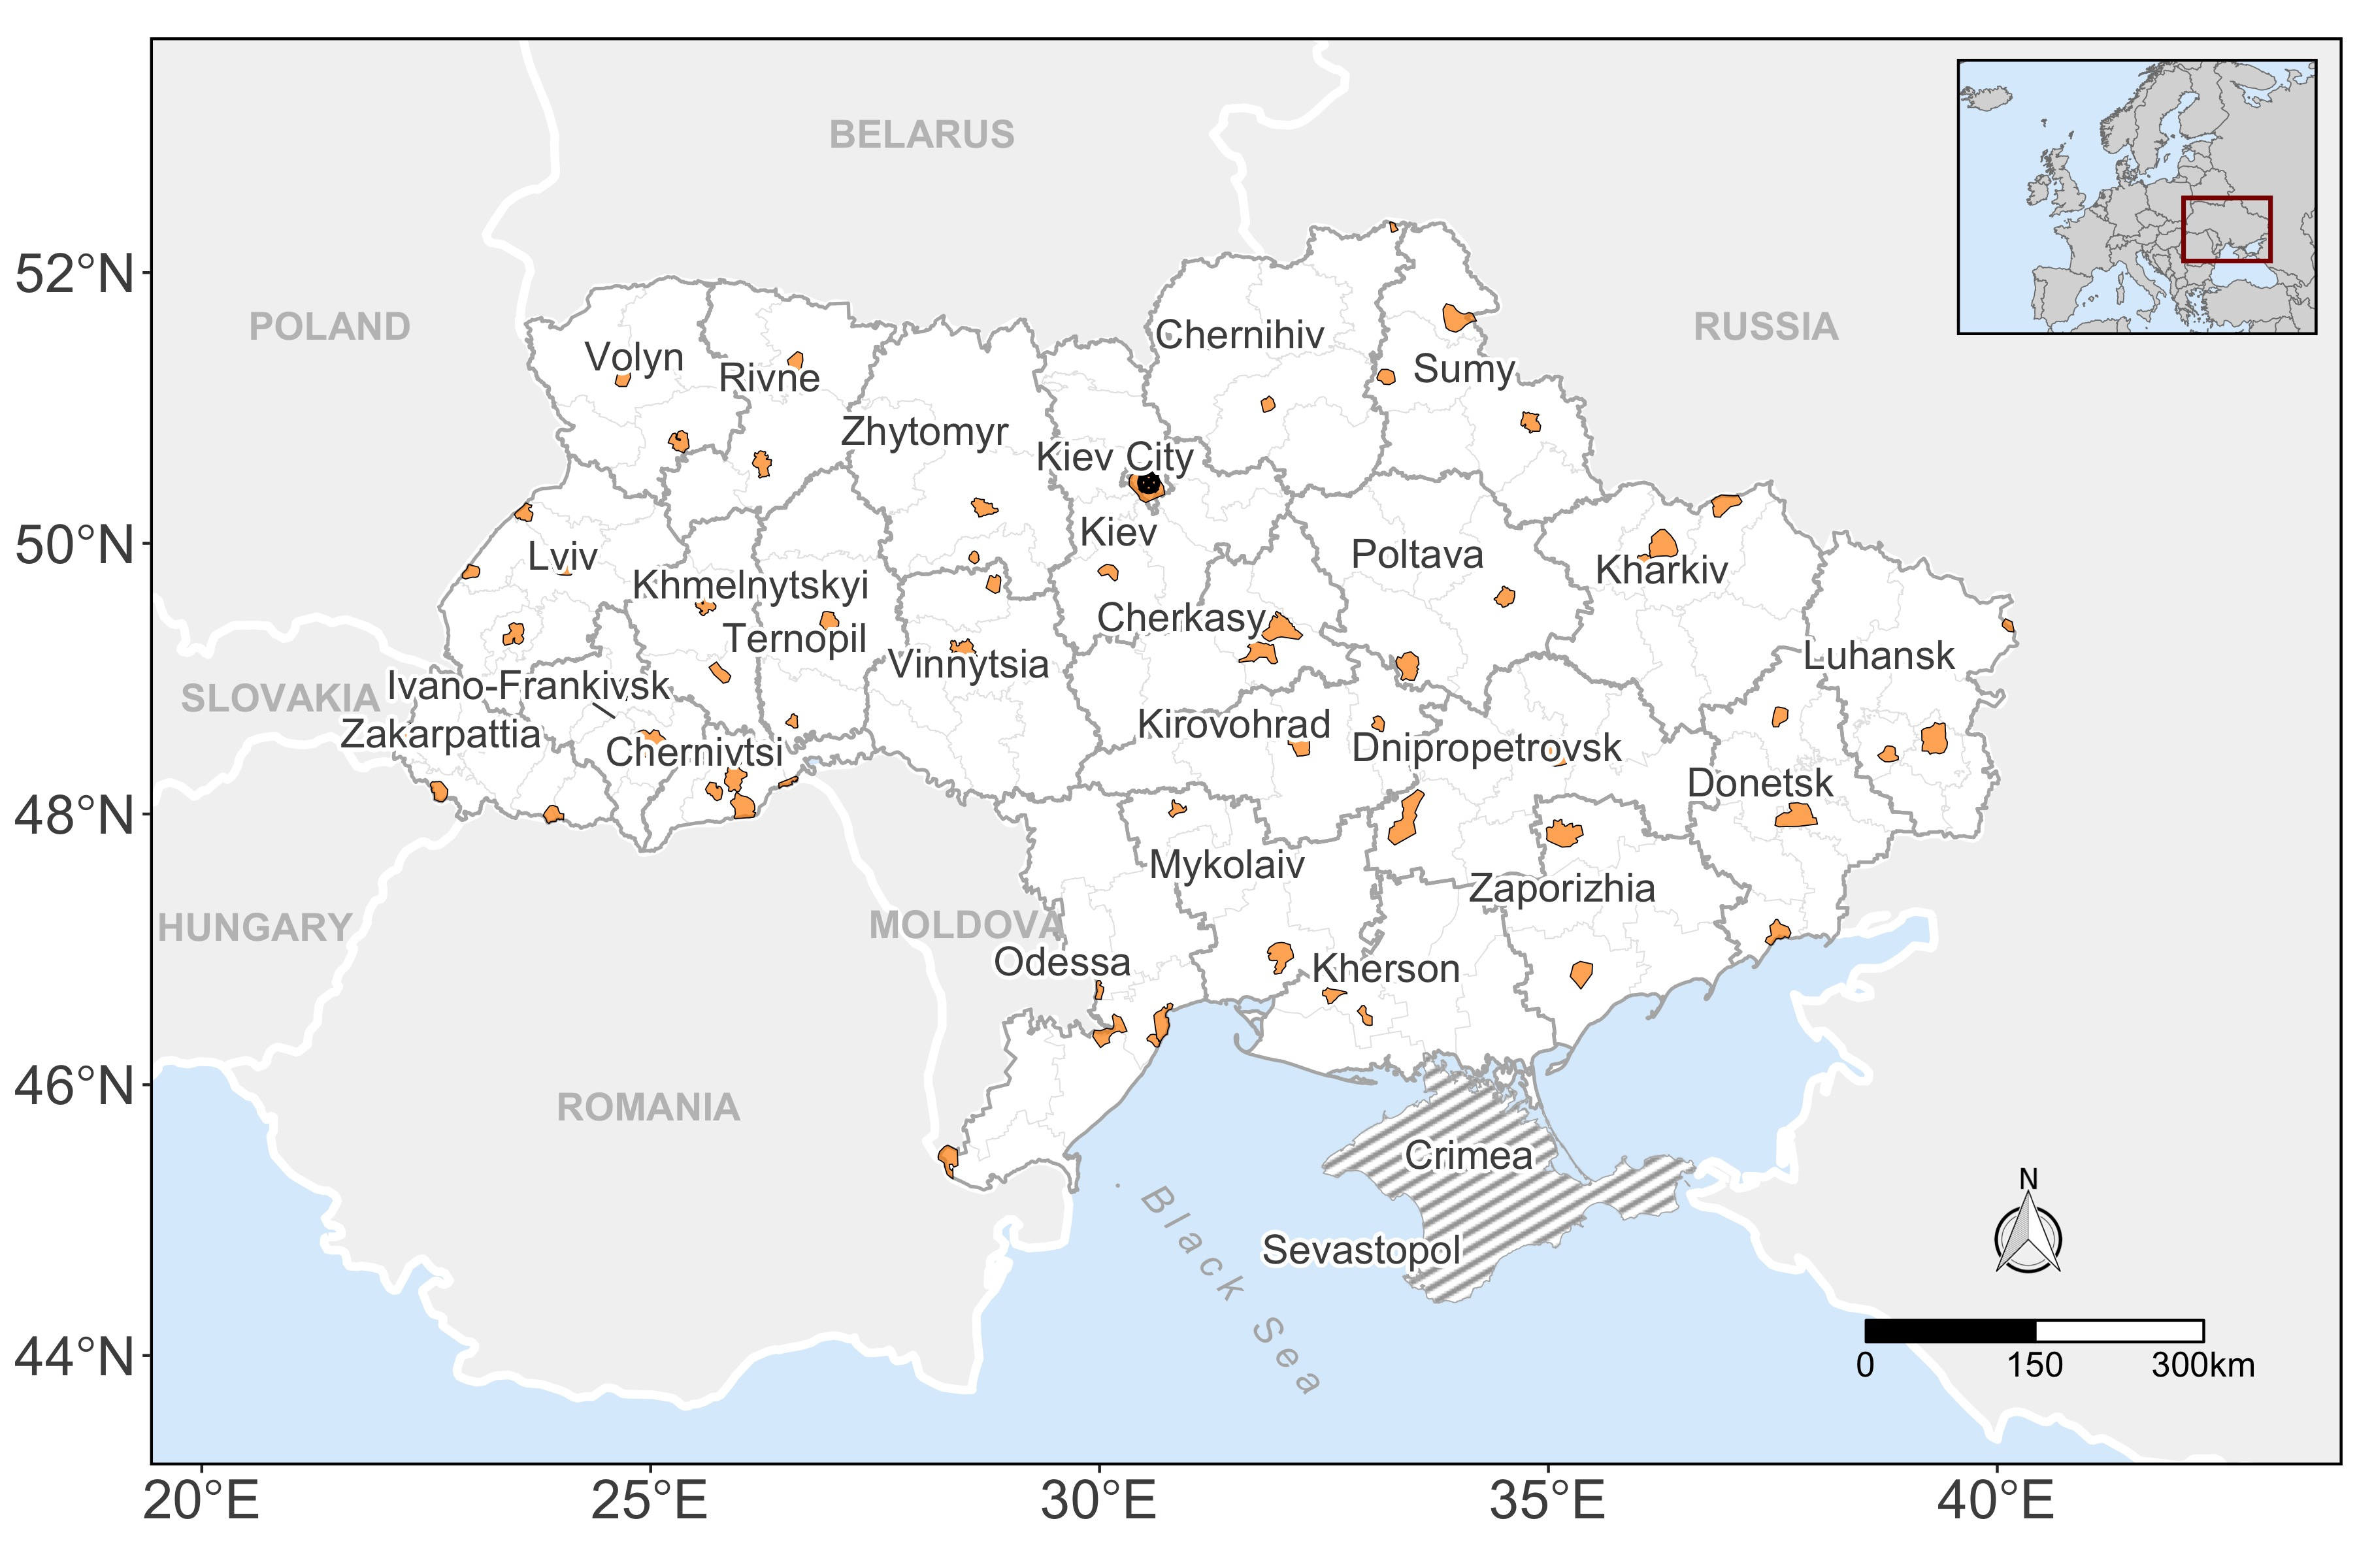
\includegraphics[width=\textwidth]{Figures/map2.jpg}
\end{center}
\caption{Map of the study region highlighting the selected areas of interest (AOI) in orange within each Ukrainian primary administrative unit (Oblast). The gray-dashed area depicts the occupied territories of Crimea and Sevastopol, both excluded from the current study.}\label{Fig_map}
\end{figure}


%%% Fig. 3 (Car density across covariates)
\begin{figure}[hbtp]
\begin{center}
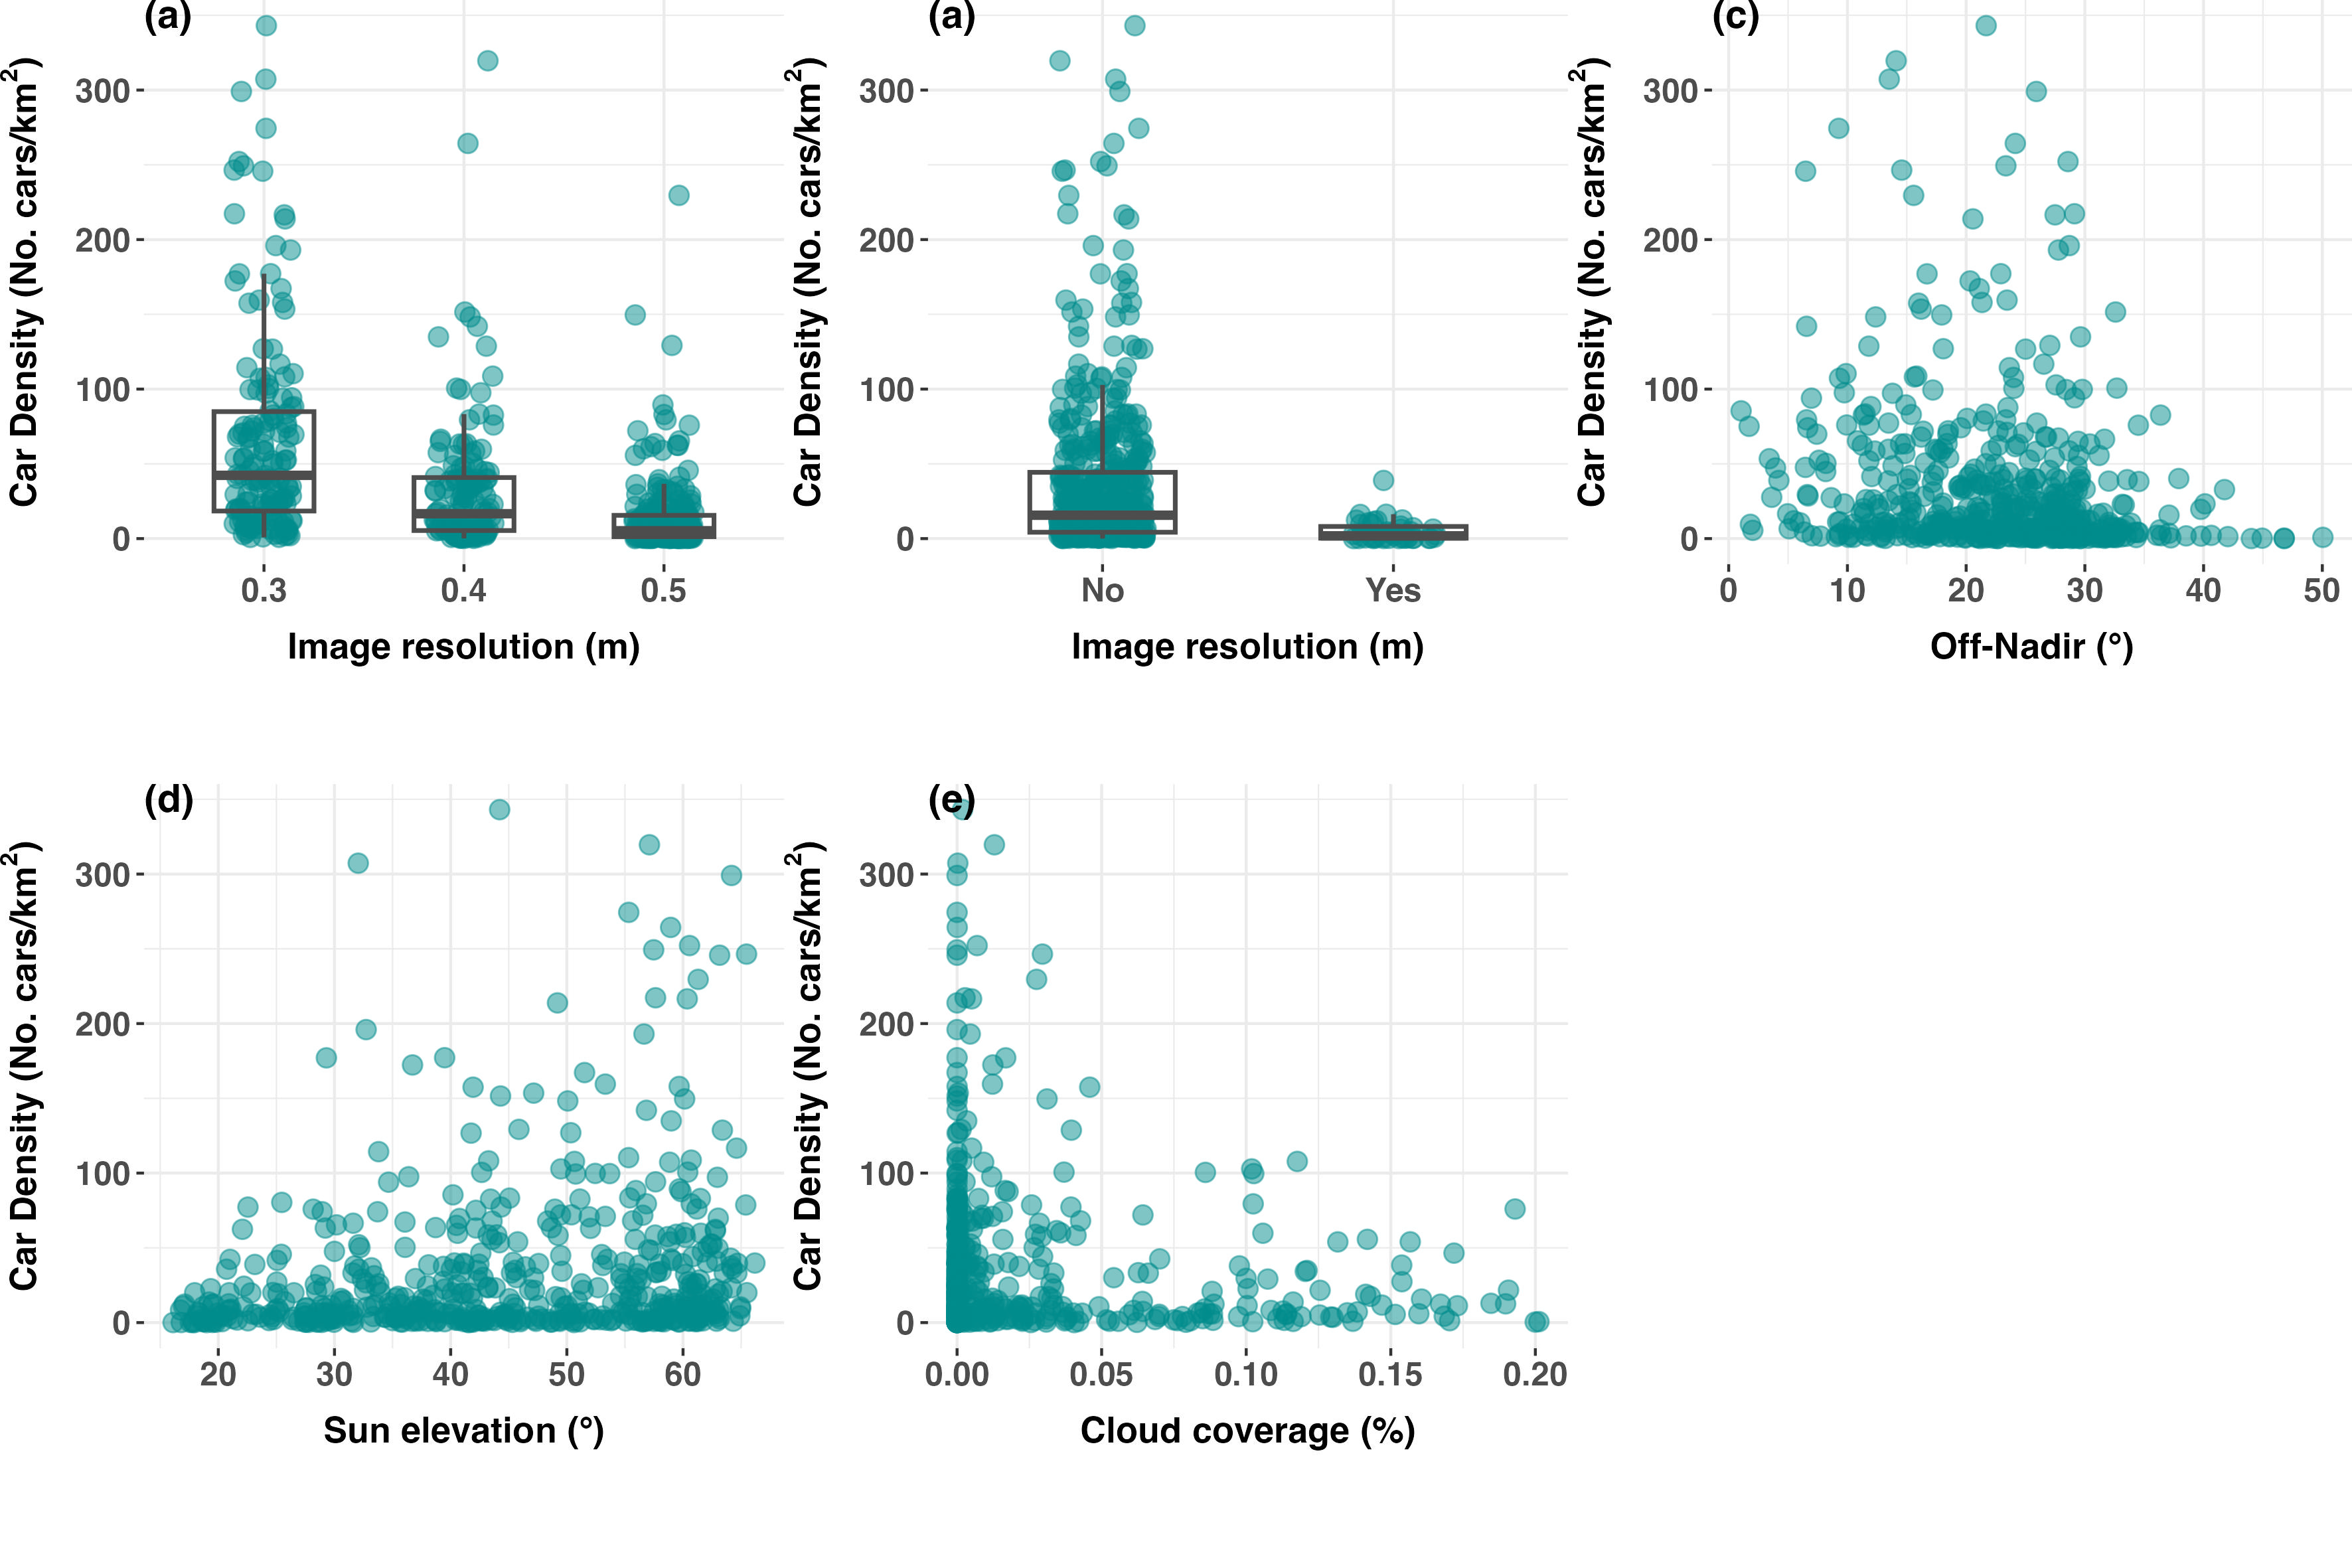
\includegraphics[width=\textwidth]{Figures/covariates.jpg}
\end{center}
\caption{Car density expressed as a function of (a) image resolution, (b) presence of snow, (c) off-Nadir angle, (d) sun elevation angle, and (e) percentage of cloud coverage.}\label{Fig_covariates}
\end{figure}


% \begin{figure}[hbtp]
% \begin{center}
% 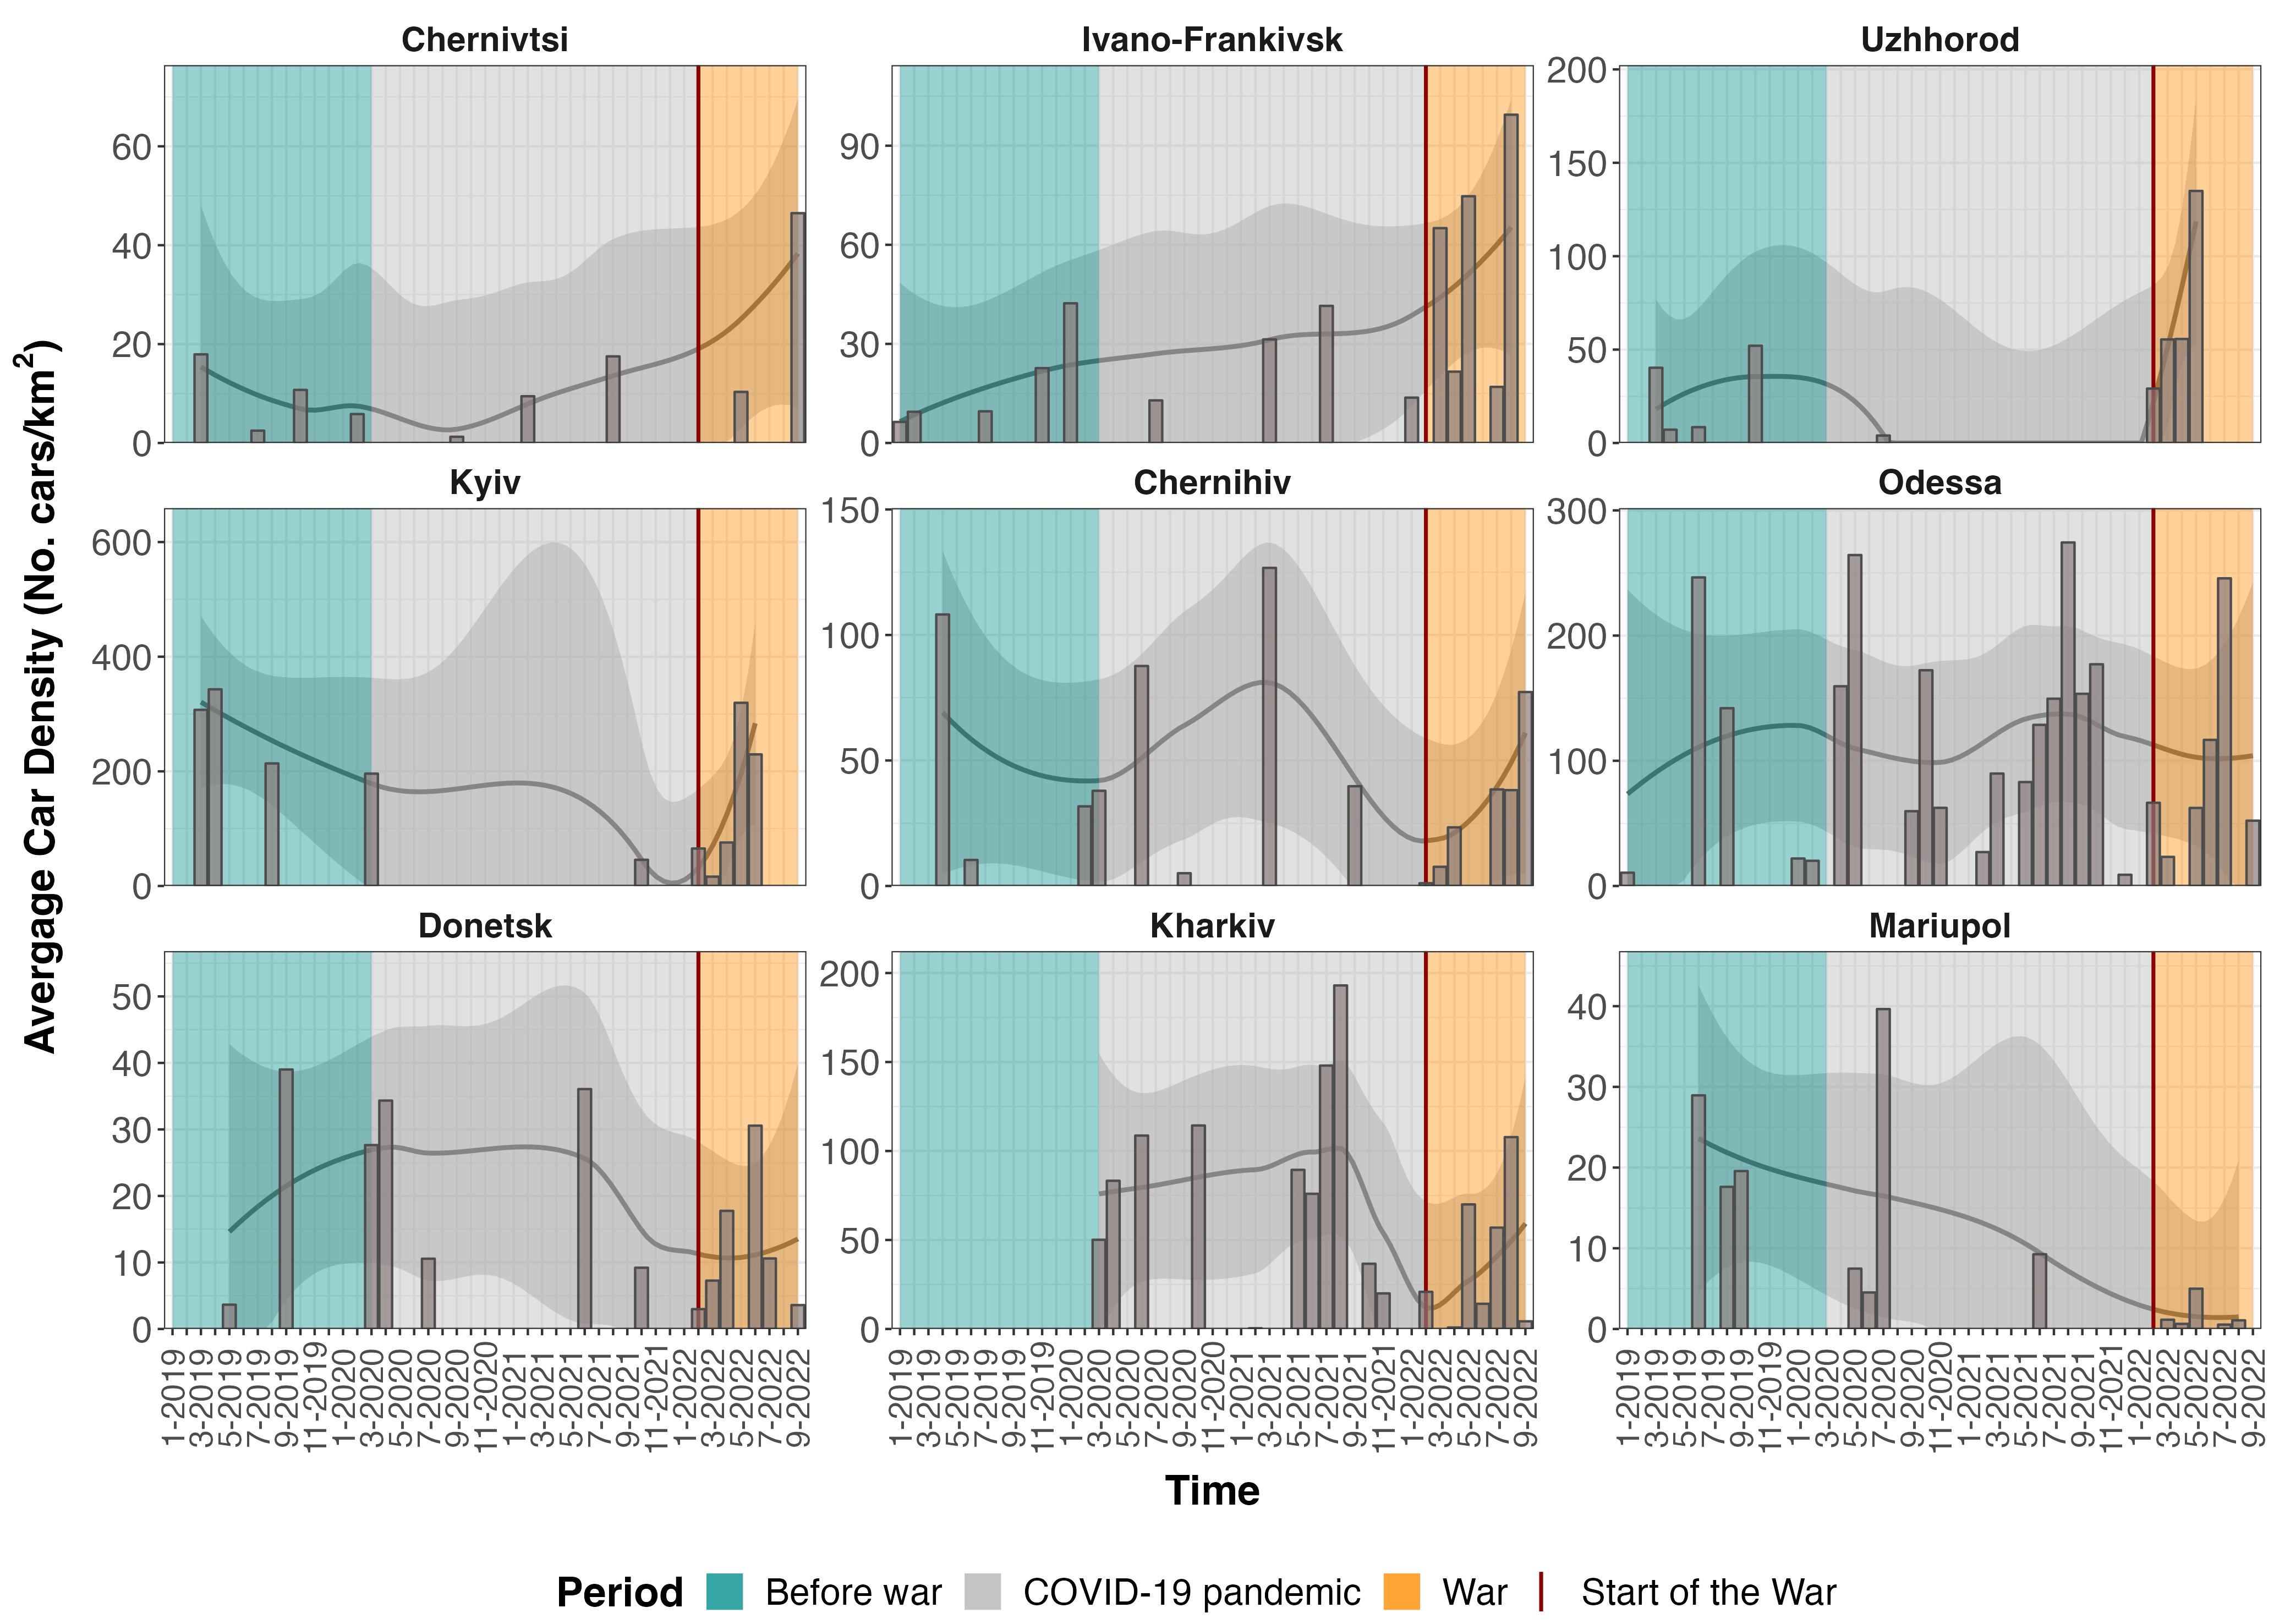
\includegraphics[width=\textwidth]{Figures/cardyn_time_main_plot.jpg}
% \end{center}
% \caption{Average car density per month for three selected cities per macro-region, with upper, mid and lower panels referring to western, central, and eastern regions, respectively. The overall trend in car density is depicted by the gray smoothed loess function with its 95\% confidence interval.  }\label{Fig_CarTempDyn}
% \end{figure}


%% Fig. 4 (Saptio-temporal car dynamics)
\begin{figure}[hbtp]
\begin{center}
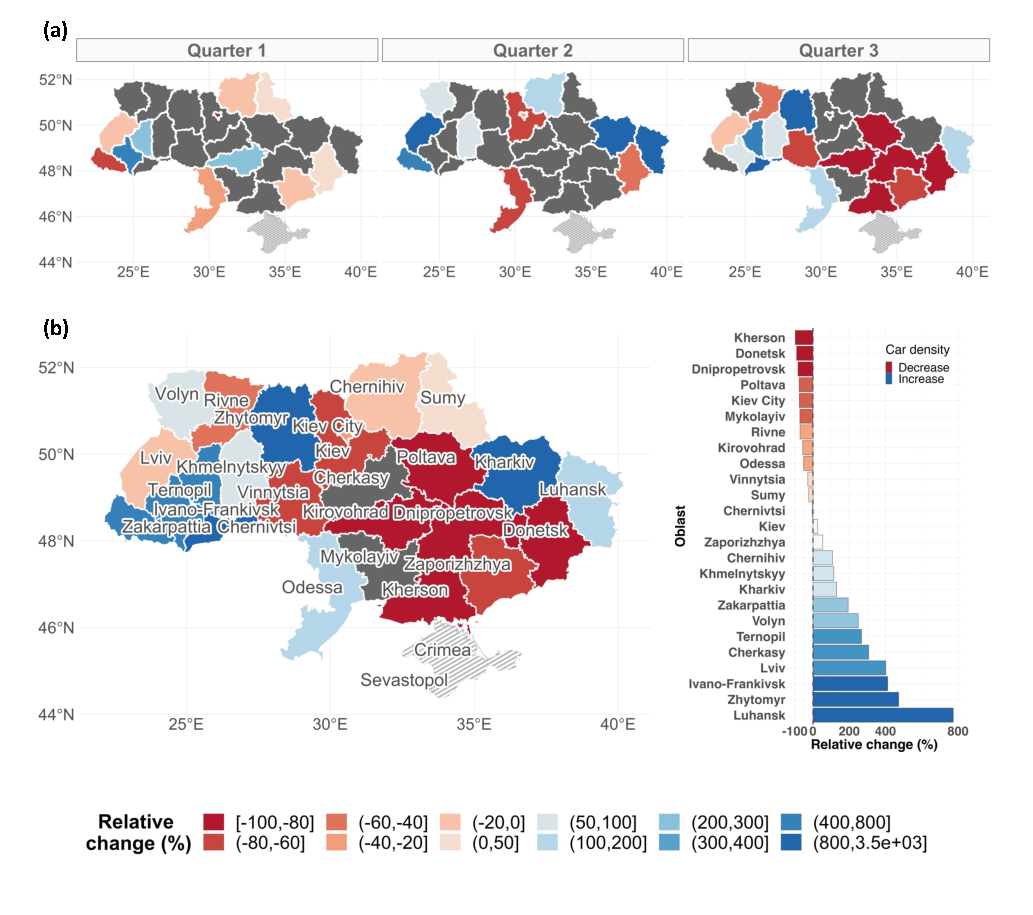
\includegraphics[width=\textwidth]{Figures/Spatial_dyn_all_updated.pdf}
\end{center}
\caption{Change in average car density for all Ukrainian primary administrative units (Oblasts) during the first year of War (2022). Values reflect the percentage change in average car density after the start of the War (24 February) relative to the baseline (2019) for either quarterly (a) or yearly (b) temporal resolution. Oblasts colored in dark gray represent cases in which the relative change could not be calculated due to missing data for either or both years. The occupied territories of Crimea and Sevastopol, depicted by the dashed area, were not considered in the current study.}\label{Fig_CarSpatDyn}
\end{figure}

%% Figure 5 (Scatterplot pop~car)
\begin{figure}[hbtp]
\begin{center}
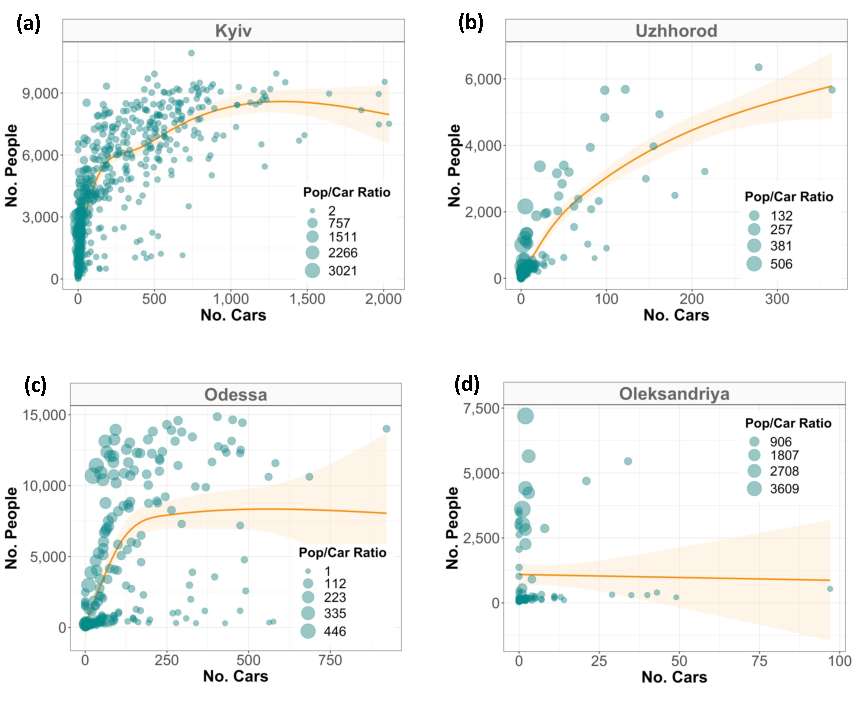
\includegraphics[width = \textwidth]{Figures/popcar_main.pdf}
\end{center}
\caption{Illustrative example of the relationship between the gridded average number of people and cars for three selected cities during the baseline year (2019). For most cities, the relationship is positive and non-linear akin to Kiev (panel a), while occasionally the relationship becomes linear as for Uzhhorod (panel b). In some rare cases, no clear relationship can be detected (e.g. Odessa, panel c), or the relationship is even fully absent (e.g. Oleksandriya, panel d). The orange smoothed function in each panel highlights the trend line from the GAM model bounded by its 95\% confidence interval, with circle sizes scaled by the population/car ratio. Each data point summarizes information from a unique grid cell (1 x 1 km) within the given city. For a complete overview, refer to Figs. \ref{figSM_PopCar_01}-\ref{figSM_PopCar_05} in the Supplementary Material.}
\label{Fig_popcar_main}
\end{figure}




%%% fig 6 IDP predictions barchart)
\begin{figure}[hbtp]
\begin{center}
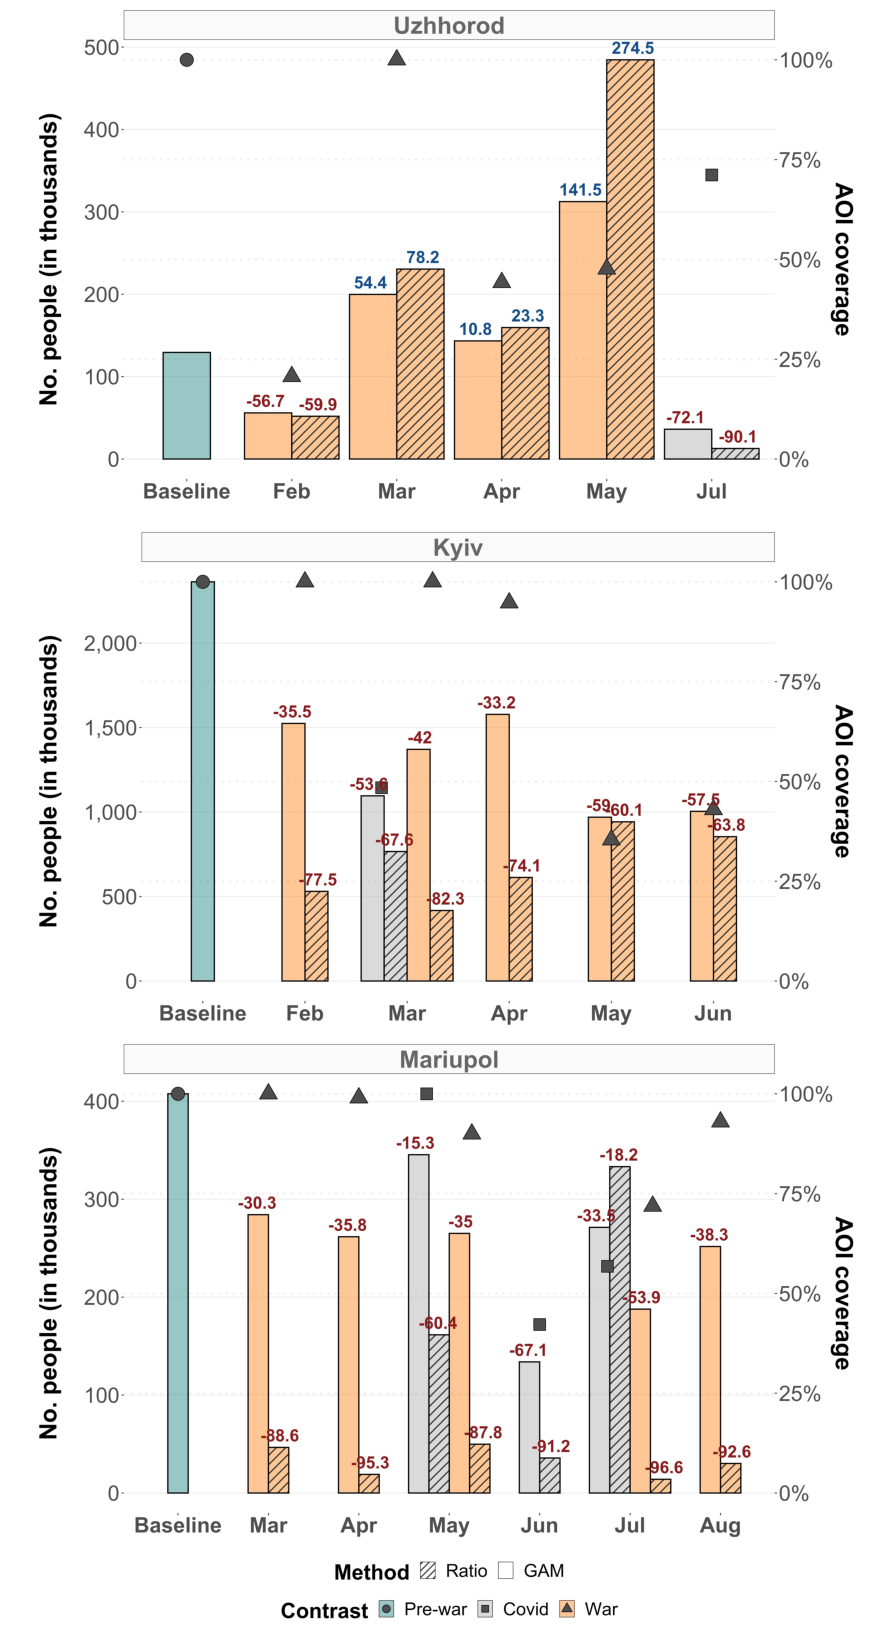
\includegraphics[scale = 0.5]{Figures/Main_IDP_pred_Figure.pdf}
\end{center}
\caption{Predictions of internally displaced people across three different cities. The turquoise bar marks the pre-War population size (2019), from which relative change in population size has been derived for the applicable months in either 2020 (first COVID-19 year, gray bars) or 2022 (War year, orange bars). Numbers on top of each bar denote the relative population change (in \%), with colors reflecting either an increase (blue) or decrease (red). Dashed and plain bars distinguish the two tested prediction methods: linear ratio (dashed) and Generalized Additive Model (GAM, plain). Moreover, the overlaid symbols, related to the secondary y-axis, depict the percentage of area covered by the satellite images underlying a given month relative to the city's area of interest (AOI).
Note that the larger population drops/increases for some cities and months should be interpreted with additional care, as it could be an artifact induced by the smaller spatial extent that is reflected by the underlying satellite images. The models for Uzhhorod, for example, predicted a population increase of up to 23\% in April 2022. This number is nevertheless likely underestimated, as the collection of satellite imagery for the given month covered less than 50\% of the city's extent (see secondary y-axis).
For the full set of results, refer to Figs. \ref{figSM_IDP_pred_Fig1}-\ref{figSM_IDP_pred_Fig5} in the Supplementary Material.}
\label{Fig_IDP_pred}
\end{figure}


%%% fig 7 (Spatial map of IDP predictions)
\begin{figure}[hbtp]
\begin{center}
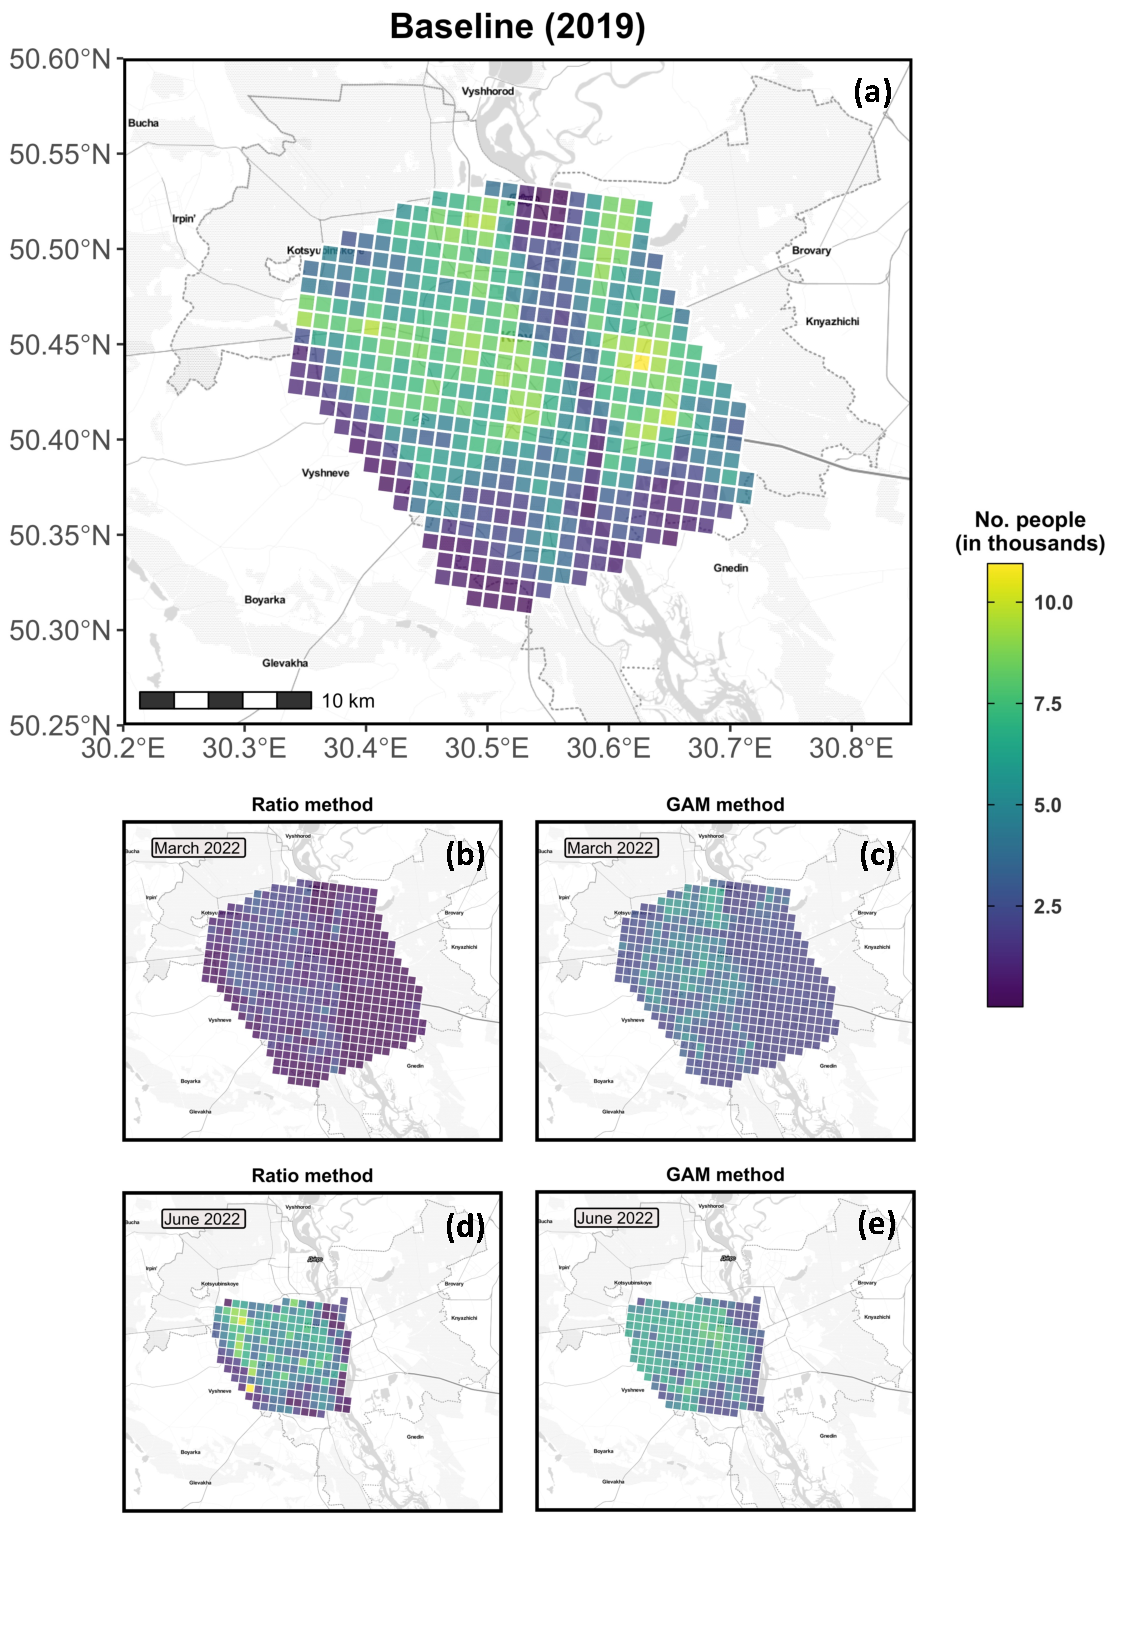
\includegraphics[scale = 0.6]{Figures/Main_gridded_predictions.pdf}
\end{center}
\caption{Gridded population for Kiev city, with each grid cell measuring 1 x 1 km. The baseline population (panel a) was retrieved from WorldPop's database, whereas the population for March and June 2022 were predicted through either the Ratio (panels b and d) or the Generalized Additive Model (GAM, panels c and e) method. Note that the satellite images underlying the month of June 2022 covered only a fraction of the city's AOI (panel a), which is also denoted in the secondary y-axis of Fig. \ref{Fig_IDP_pred}. To interpret the present figure in relative terms, refer to Fig. \ref{figSM_gridded_pred} in the Supplementary Material.}
\label{Fig_gridded_pred}
\end{figure}


\clearpage
\section*{Tables}\label{Tables}



%% GLM table %%
%%%%%%%%%%%%%%%
\begin{table}[hbtp]
 \caption{Statistical summary of the Generalized Linear Model (GLM) conducted to test for the effect of imagery-related features on car density. Estimated parameters are on a log-scale and include the 95\% confidence interval, t-values, and p-values expressed at 5\% of level of significance. }    
\label{GLM_Table}

\begin{tabular}{lccccc}
\toprule
\multicolumn{1}{l}{\textbf{Parameters}} & \textbf{Estimate} & \textbf{2.5\%} & \textbf{97.5\%} & \textbf{t-value} & \textbf{P-value} \\ \midrule
Intercept                               & 3.44              & 2.85           & 4.02            & 11.55            & \textless 0.05   \\
Image resolution - 0.4                  & -1.05             & -1.37          & -0.73           & -6.45            & \textless 0.05   \\
Image resolution - 0.5                  & -1.90             & -2.20          & -1.61           & -12.59           & \textless 0.05   \\
Snow presence - Yes                      & -1.67             & -2.16          & -1.18           & -6.72            & \textless 0.05   \\
Off-Nadir                               & -0.03             & -0.05          & -0.02           & -3.99            & \textless 0.05   \\
Sun elevation                           & 0.02              & 0.01           & 0.03            & 4.49             & \textless 0.05   \\ 
Cloud coverage                          & -1.74             & -4.55          & 1.07            & -1.22            & 0.225            \\ \bottomrule
\end{tabular}
\end{table}


\clearpage
\backmatter

\bmhead{Supplementary information}
%% See example from: https://www.nature.com/articles/s41562-023-01533-9#Sec20



\bmhead{Acknowledgments}
Part of this work was done while MCR and IW were employed at the Qatar Computing Research Institute. All authors thank the Qatar Computing Research Institute for providing funding for procuring the satellite imagery from Maxar. Furthermore, we thank Maxar for 
granting the sample images displayed in this research article. Special thanks to Katherine Hoffmann Pham for all constructive comments on an earlier versions. 




\section*{Declarations}

% Some journals require declarations to be submitted in a standardised format. Please check the Instructions for Authors of the journal to which you are submitting to see if you need to complete this section. If yes, your manuscript must contain the following sections under the heading `Declarations':

% \begin{itemize}
% \item Funding
% \item Conflict of interest/Competing interests (check journal-specific guidelines for which heading to use)
% \item Ethics approval 
% \item Consent to participate
% \item Consent for publication
% \item Availability of data and materials
% \item Code availability 
% \item Authors' contributions
% \end{itemize}
% \noindent
% If any of the sections are not relevant to your manuscript, please include the heading and write `Not applicable' for that section. 

\subsection*{Funding}
The authors declare that there were no funding involved in this research.

\subsection*{Competing interests}
The authors declare no competing interests.

%\subsection*{Ethics approval}
%Not applicable.

%\subsection*{Consent to participate}
%Not applicable. 

%\subsection*{Consent for publication}
%\textcolor{orange}{Include here the MAXAR licensing}

\subsection*{Data Availability}
All data underlying the findings of the present study are available on the first author's GitHub
repository (\url{https://github.com/mcruf/IDP_UKR}). However, we note that the original Maxar satellite imagery cannot be openly shared due to confidentiality reasons. 


\subsection*{Code Availability}
All codes underlying the analyses and figures are stored in the first author's GitHub repository (\url{https://github.com/mcruf/IDP_UKR}).The code used for car detection can be found at the original developer's GitHub repository (\url{https://github.com/maups/covid19-satellite-analysis}).


\subsection*{Authors' contributions}
IW and FO conceptualized the study, with supportive contribution of MCR on its research design. MF performed the satellite data collection and imagery pre-processing. FO conducted the Machine Learning analysis. MR conducted all data post-processing. MR analyzed the data, with supportive contribution from IW and FO. All authors wrote the first draft of the manuscript, and read and approved the submitted version.


%%%%%%%%%%%%%%%%%%%%%%%%%%%%%%%%%%%%%
%%%%%  Supplementary Material  %%%%%
%%%%%%%%%%%%%%%%%%%%%%%%%%%%%%%%%%%%%
\newpage
\begin{appendices}

\section{Supplementary Tables}\label{SuppMat_tabs}


% Goodness-of-fit summary from the GAM model
%%%%%%%%%%%%%%%%%%%%%%%%%%%%%%%%%%%%%%
\begin{table}[hbtp]
\caption{Goodness-of-fit statistics of the Generalized Additive Models (GAMs) applied to the baseline year.}
\label{SM_GAM_Table}
\begin{tabular}{lc}
\toprule
\multicolumn{1}{l}{\textbf{City}} & \textbf{\bm{$R^2$}(adj.)} \\ \midrule
% \begin{tabular}{ p{6cm} p{6cm} lc}
% \hline
% \multicolumn{1}{c}{\textbf{City}}   &  \textbf{\bm{$R^2$}(adj.)} 
% \hline
Alchevsk                          & 0.30          \\
Berehove                          & 0.63          \\
Bila-Tserkva                      & 0.83          \\
Cherkasy                          & 0.74          \\
Chernihiv                         & 0.62          \\
Chernivtsi                        & 0.65          \\
Dnipro                            & 0.35          \\
Donetsk                           & 0.60          \\
Ivano-Frankivsk                   & 0.83          \\
Kamyanets-Podilskyi               & 0.75          \\
Kherson                           & 0.50          \\
Khmelnytskyi                      & 0.67          \\
Konotop                           & 0.60          \\
Kovel                             & 0.65          \\
Kramatorsk                        & 0.54          \\
Kremenchuk                        & 0.47          \\
Kropyvnytskyi                     & 0.54          \\
Kuchurhan                         & 0.61          \\
Kyiv                              & 0.63          \\
Luhansk                           & 0.62          \\
Lutsk                             & 0.71          \\
Lviv                              & 0.52          \\
Mamalyha                          & 0.21          \\
Mariupol                          & 0.37          \\
Melitopol                         & 0.23          \\
Merefa                            & 0.66          \\
Mykolaiv                          & 0.61          \\
Odessa                            & 0.35          \\
Oleksandriya                      & -0.04         \\
Pervomaisk                        & 0.75          \\
Pletenivka                        & 0.74          \\
Poltava                           & 0.61          \\
Reni                              & 0.50          \\
Rivne                             & 0.79          \\
Shehyni                           & 0.26          \\
Solotvino                         & 0.53          \\
Sumy                              & 0.63          \\
Ternopil                          & 0.55          \\
Uzhhorod                          & 0.75          \\
Velykodolynske                    & 0.47          \\
Vinnytsia                         & 0.67          \\
Zaporizhia                        & 0.45          \\
Zhytomyr                          & 0.68          \\ \bottomrule
\end{tabular}
\end{table}



% Summary of selected AOIs
%%%%%%%%%%%%%%%%%%%%%%%%%%%%

% \begin{longtable}{lllr}
% \caption{List of the evaluated Ukrainian cities.}
%     \label{SM_AOI_Table}
% \\
% \toprule
% \multicolumn{1}{l}{\textbf{City}} & \multicolumn{1}{l}{\textbf{Oblast}} & \multicolumn{1}{l}{\textbf{Region}} & \multicolumn{1}{r}{\textbf{AOI area (km$^2$)}} \\ \midrule
% Alchevsk                          & Luhansk                             & East                                & 149.4  \\
% Berdychiv                         & Zhytomyr                            & Central                             & 58.9    \\
% Berehove                          & Zakarpattia                         & West                                & 170.5   \\
% Bila-Tserkva                      & Kiev                                & Central                             & 130.4                                       \\
% Cherkasy                          & Cherkasy                            & Central                             & 419.0                                       \\
% Chernihiv                         & Chernihiv                           & Central                             & 122.0                                       \\
% Chernivtsi                        & Chernivtsi                          & West                                & 288.7                                       \\
% Chortkiv                          & Ternopil                            & West                                & 147.1                                       \\
% Dnipro                            & Dnipropetrovsk                      & East                                & 506.7                                       \\
% Donetsk                           & Donetsk                             & East                                & 483.3                                       \\
% Drohobych                         & Lviv                                & West                                & 212.5                                       \\
% Hremiach                          & Chernihiv                           & Central                             & 31.7                                        \\
% Ivano-Frankivsk                   & Ivano-Frankivsk                     & West                                & 163.3                                       \\
% Kamyanets-Podilskyi               & Khmelnytskyy                        & West                                & 69.9                                        \\
% Katerynivka                       & Sumy                                & Central                             & 344.8                                       \\
% Kharkiv                           & Kharkiv                             & East                                & 398.4                                       \\
% Kherson                           & Kherson                             & Central                             & 135.3                                       \\
% Khmelnytskyi                      & Khmelnytskyy                        & West                                & 175.1                                       \\
% Kolomyiska                        & Ivano-Frankivsk                     & West                                & 523.2                                       \\
% Konotop                           & Sumy                                & Central                             & 135.3                                       \\
% Kovel                             & Volyn                               & West                                & 131.4                                       \\
% Kozyatyn                          & Vinnytsia                           & Central                             & 127.2                                       \\
% Kramatorsk                        & Donetsk                             & East                                & 155.8                                       \\
% Kremenchuk                        & Poltava                             & Central                             & 313.2                                       \\
% Kropyvnytskyi                     & Kirovohrad                          & Central                             & 223.7                                       \\
% KryvyiRih                         & Dnipropetrovsk                      & Central                             & 608.2                                       \\
% Kuchurhan                         & Odessa                              & Central                             & 74.3                                        \\
% Kyiv                              & Kiev                                & Central                             & 525.0                                       \\
% Luhansk                           & Luhansk                             & East                                & 452.2                                       \\
% Lutsk                             & Volyn                               & West                                & 190.0                                       \\
% Lviv                              & Lviv                                & West                                & 205.0                                       \\
% Mamalyha                          & Chernivtsi                          & West                                & 64.5                                        \\
% Mariupol                          & Donetsk                             & East                                & 237.0                                       \\
% Melitopol                         & Zaporizhzhya                        & East                                & 281.9                                       \\
% Merefa                            & Kharkiv                             & East                                & 139.2                                       \\
% Milove                            & Luhansk                             & East                                & 69.1                                        \\
% Mykolaiv                          & Mykolayiv                           & Central                             & 350.4                                       \\
% Nizhyn                            & Chernihiv                           & Central                             & 97.0                                        \\
% Odessa                            & Odessa                              & Central                             & 269.1                                       \\
% Oleksandriya                      & Kirovohrad                          & Central                             & 91.9                                        \\
% Pervomaisk                        & Mykolayiv                           & Central                             & 96.4                                        \\
% Pletenivka                        & Kharkiv                             & East                                & 273.0                                       \\
% Poltava                           & Poltava                             & East                                & 174.2                                       \\
% Porubne                           & Chernivtsi                          & West                                & 301.3                                       \\
% Rava-Ruska                        & Lviv                                & West                                & 134.6                                       \\
% Reni                              & Odessa                              & Central                             & 267.1                                       \\
% Rivne                             & Rivne                               & West                                & 200.9                                       \\
% Sarny                             & Rivne                               & West                                & 135.7                                       \\
% Shehyni                           & Lviv                                & West                                & 113.5                                       \\
% Smila                             & Cherkasy                            & Central                             & 334.9                                       \\
% Solotvino                         & Zakarpattia                         & West                                & 153.0                                       \\
% Storozhynets                      & Chernivtsi                          & West                                & 132.2                                       \\
% Sumy                              & Sumy                                & East                                & 179.5                                       \\
% Ternopil                          & Ternopil                            & West                                & 139.8                                       \\
% Udobne                            & Odessa                              & Central                             & 296.4                                       \\
% Uzhhorod                          & Zakarpattia                         & West                                & 245.9                                       \\
% Velyki-Kopani                     & Kherson                             & Central                             & 105.4                                       \\
% Velykodolynske                    & Odessa                              & Central                             & 69.7                                        \\
% Vinnytsia                         & Vinnytsia                           & Central                             & 214.1                                       \\
% Zaporizhzhia                      & Zaporizhzhya                        & East                                & 472.8                                       \\
% Zhytomyr                          & Zhytomyr                            & Central                             & 183.9    
% \\
% \bottomrule
% \end{longtable}


\begin{longtable}{lllccc}
\caption{List of the selected cities with descriptive statistics relative to their satellite imagery coverage. The AOI defines roughly the city's perimeter, whereby the downloaded satellite images might or not cover the full AOI area. On average, most cities were well covered by the downloaded images. Berdychiv was the only city with only one available image, thus the NA in the table.}
\label{SM_AOI_Table}
\\
\toprule
\multicolumn{1}{l}{\textbf{City}} & \multicolumn{1}{l}{\textbf{Oblast}} & \multicolumn{1}{l}{\textbf{Region}} & \multicolumn{1}{r}{\textbf{AOI area (km$^2$)}} & \multicolumn{1}{l}{\textbf{Mean}} & \multicolumn{1}{l}{\textbf{Std. Dev.}} \\ \midrule
Alchevsk            & Luhansk         & East    & 161.5                                & 69.7  & 53.1      \\
Berdychiv           & Zhytomyr        & Central & 62.8                                 & 62.8  & NA        \\
Berehove            & Zakarpattia     & West    & 184.3                                & 90.4  & 59.0      \\
Bila-Tserkva        & Kiev            & Central & 142.7                                & 113.2 & 40.2      \\
Cherkasy            & Cherkasy        & Central & 444.3                                & 206.2 & 126.3     \\
Chernihiv           & Chernihiv       & Central & 128.3                                & 125.8 & 37.3      \\
Chernivtsi          & Chernivtsi      & West    & 310.5                                & 282.3 & 81.7      \\
Chortkiv            & Ternopil        & West    & 64.8                                 & 24.4  & 20.9      \\
Dnipro              & Dnipropetrovsk  & East    & 525.5                                & 273.3 & 169.7     \\
Donetsk             & Donetsk         & East    & 509.3                                & 149.2 & 146.9     \\
Drohobych           & Lviv            & West    & 230.4                                & 209.4 & 30.6      \\
Hremiach            & Chernihiv       & Central & 34.7                                 & 16.5  & 11.9      \\
Ivano-Frankivsk     & Ivano-Frankivsk & West    & 178.7                                & 132.6 & 40.7      \\
Kamyanets-Podilskyi & Khmelnytskyy    & West    & 74.5                                 & 74.5  & 1.1       \\
Katerynivka         & Sumy            & Central & 364.0                                & 207.6 & 92.1      \\
Kharkiv             & Kharkiv         & East    & 418.1                                & 215.9 & 115.9     \\
Kherson             & Kherson         & Central & 142.8                                & 81.9  & 47.9      \\
Khmelnytskyi        & Khmelnytskyy    & West    & 188.1                                & 101.4 & 66.0      \\
Kolomyiska          & Ivano-Frankivsk & West    & 324.9                                & 220.1 & 93.6      \\
Konotop             & Sumy            & Central & 145.4                                & 145.4 & 49.7      \\
Kovel               & Volyn           & West    & 141.4                                & 125.4 & 35.2      \\
Kozyatyn            & Vinnytsia       & Central & 139.1                                & 75.3  & 90.2      \\
Kramatorsk          & Donetsk         & East    & 167.7                                & 104.5 & 53.6      \\
Kremenchuk          & Poltava         & Central & 332.6                                & 164.2 & 117.2     \\
Kropyvnytskyi       & Kirovohrad      & Central & 240.2                                & 165.8 & 67.3      \\
KryvyiRih           & Dnipropetrovsk  & Central & 643.2                                & 290.5 & 214.7     \\
Kuchurhan           & Odessa          & Central & 71.9                                 & 61.5  & 22.0      \\
Kyiv                & Kiev            & Central & 569.7                                & 201.1 & 186.0     \\
Luhansk             & Luhansk         & East    & 475.9                                & 72.9  & 153.8     \\
Lutsk               & Volyn           & West    & 207.5                                & 186.9 & 57.7      \\
Lviv                & Lviv            & West    & 217.0                                & 109.7 & 76.3      \\
Mamalyha            & Chernivtsi      & West    & 70.1                                 & 51.2  & 27.0      \\
Mariupol            & Donetsk         & East    & 257.7                                & 164.2 & 89.8      \\
Melitopol           & Zaporizhzhya    & East    & 298.9                                & 227.7 & 84.1      \\
Merefa              & Kharkiv         & East    & 153.0                                & 64.9  & 63.2      \\
Milove              & Luhansk         & East    & 73.2                                 & 40.3  & 24.0      \\
Mykolaiv            & Mykolayiv       & Central & 374.7                                & 131.6 & 113.6     \\
Nizhyn              & Chernihiv       & Central & 101.9                                & 99.0  & 29.3      \\
Odessa              & Odessa          & Central & 292.0                                & 194.4 & 78.7      \\
Oleksandriya        & Kirovohrad      & Central & 97.0                                 & 97.0  & 36.2      \\
Pervomaisk          & Mykolayiv       & Central & 103.2                                & 53.3  & 37.3      \\
Pletenivka          & Kharkiv         & East    & 255.1                                & 100.8 & 81.4      \\
Poltava             & Poltava         & East    & 190.2                                & 187.5 & 51.3      \\
Porubne             & Chernivtsi      & West    & 225.8                                & 122.1 & 75.3      \\
Rava-Ruska          & Lviv            & West    & 147.7                                & 83.6  & 51.7      \\
Reni                & Odessa          & Central & 288.7                                & 89.5  & 79.2      \\
Rivne               & Rivne           & West    & 219.7                                & 210.8 & 84.7      \\
Sarny               & Rivne           & West    & 146.4                                & 146.4 & 0.5       \\
Shehyni             & Lviv            & West    & 124.1                                & 83.6  & 42.4      \\
Smila               & Cherkasy        & Central & 361.1                                & 208.4 & 78.9      \\
Solotvino           & Zakarpattia     & West    & 163.4                                & 108.3 & 59.5      \\
Storozhynets        & Chernivtsi      & West    & 104.9                                & 39.8  & 31.1      \\
Sumy                & Sumy            & East    & 195.7                                & 182.6 & 75.4      \\
Ternopil            & Ternopil        & West    & 149.6                                & 114.0 & 28.9      \\
Udobne              & Odessa          & Central & 198.3                                & 107.2 & 58.4      \\
Uzhhorod            & Zakarpattia     & West    & 263.4                                & 145.3 & 77.8      \\
Velyki-Kopani       & Kherson         & Central & 96.3                                 & 40.9  & 37.5      \\
Velykodolynske      & Odessa          & Central & 74.5                                 & 48.0  & 27.8      \\
Vinnytsia           & Vinnytsia       & Central & 225.1                                & 198.4 & 75.9      \\
Zaporizhzhia        & Zaporizhzhya    & East    & 499.6                                & 204.8 & 172.4     \\
Zhytomyr            & Zhytomyr        & Central & 198.7                                & 105.1 & 71.3     \\ 
\bottomrule
\end{longtable}



% Car detection confidence threshold summary results
%%%%%%%%%%%%%%%%%%%
\begin{table}
\centering
\caption{Summary of results achieved by the car detection model in terms of Precision, Recall, and F$_{0.5}$-Score across varying confidence thresholds.}
\label{SM_Conf_Thr_Table}
\begin{tabular}{cccc}
\toprule
\textbf{Confidence} & \textbf{Precision} & \textbf{Recall} & \textbf{F$_{0.5}$-Score} \\
\midrule
0.00 & 0.0821 & 0.8199 & 0.1001 \\
0.05 & 0.0821 & 0.8199 & 0.1001 \\
0.10 & 0.2408 & 0.6605 & 0.2758 \\
0.15 & 0.3614 & 0.5413 & 0.3871 \\
0.20 & 0.4165 & 0.4760 & 0.4272 \\
0.25 & 0.4542 & 0.4302 & 0.4492 \\
0.30 & 0.4858 & 0.3933 & 0.4640 \\
0.35 & 0.5119 & 0.3611 & 0.4724 \\
0.40 & 0.5343 & 0.3318 & 0.4762 \\
\textbf{0.45} & \textbf{0.5578} & \textbf{0.3032} & \textbf{0.4776} \\
0.50 & 0.5745 & 0.2761 & 0.4724 \\
0.55 & 0.5926 & 0.2489 & 0.4644 \\
0.60 & 0.6117 & 0.2252 & 0.4553 \\
0.65 & 0.6319 & 0.1992 & 0.4406 \\
0.70 & 0.6563 & 0.1720 & 0.4199 \\
0.75 & 0.6807 & 0.1424 & 0.3877 \\
0.80 & 0.7045 & 0.1100 & 0.3386 \\
0.85 & 0.7390 & 0.0753 & 0.2675 \\
0.90 & 0.7556 & 0.0374 & 0.1560 \\
0.95 & 0.8228 & 0.0034 & 0.0168 \\
1.00 & 0.0000 & 0.0000 & 0.0000 \\
\bottomrule
\end{tabular}
\end{table}



% OSM tag summary
%%%%%%%%%%%%%%%%%%%
\begin{table}

    \caption{Summary of the Open Street Maps (OSM) tags retrieved for the  false-positives filtering process. For a full description of each OSM tag, refer to \url{https://wiki.openstreetmap.org/wiki/Map_features}}
    \label{SM_OSM_Table}
    
 
    \begin{tabular}{ll}
    \toprule
    \multicolumn{1}{l}{\textbf{Key}} & \multicolumn{1}{l}{\textbf{Value}} \\ \midrule
    \multirow{11}{*}{Landuse}        & Farmland                                                            \\
                                     & Farmyard                           \\
                                     & Vineyard                           \\
                                     & Forest                             \\
                                     & Grass                              \\
                                     & Scrub                              \\
                                     & Meadow                             \\
                                     & Heath                              \\
                                     & Railway station                    \\
                                     & Railway                            \\
                                     & Industrial                         \\ \midrule
    Place                            & Sea                                \\ \midrule
    \multirow{6}{*}{Natural}         & Grassland                         
                               \\
                               & Water                             
                               \\
                               & Wetland                          
                               \\
                               & Scrub                            
                               \\
                               & Wood                          
                               \\
                               & Bay                                
                               \\ \midrule
    Leisure                    & Park                               
    \\ \midrule
    \multirow{2}{*}{Aeroway}         & Aerodrome                          
                               \\
                               & Apron                              
                               \\ \bottomrule
\end{tabular}
\end{table}















\clearpage
\section{Supplementary Figures}\label{SuppMat_figs}

% No. of images across time of the day
%%%%%%%%%%%%%%%%%%%%%%%%%%%%%%%%%%%%%%%%
\begin{figure}[htbp]
\begin{center}
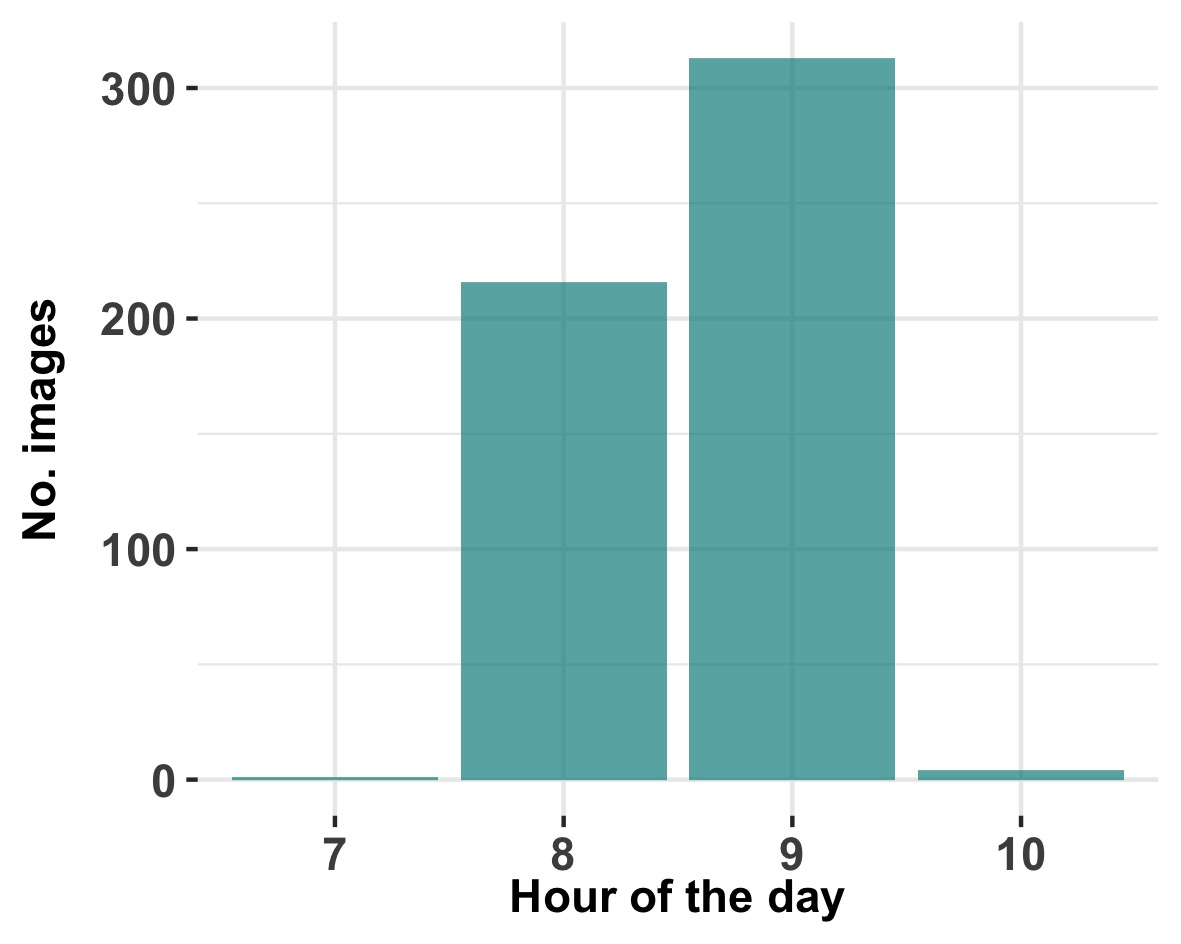
\includegraphics[width=0.70\textwidth]{Figures/hour_of_day.jpg}
\end{center}
\caption{Number of satellite images per hour of the day (UTC time zone).}
\label{figSM_Nimages_per_hour}
\end{figure}


% Data availability over space
%%%%%%%%%%%%%%%%%%%%%%%%%%%%%%
\begin{figure}[htbp]
\begin{center}
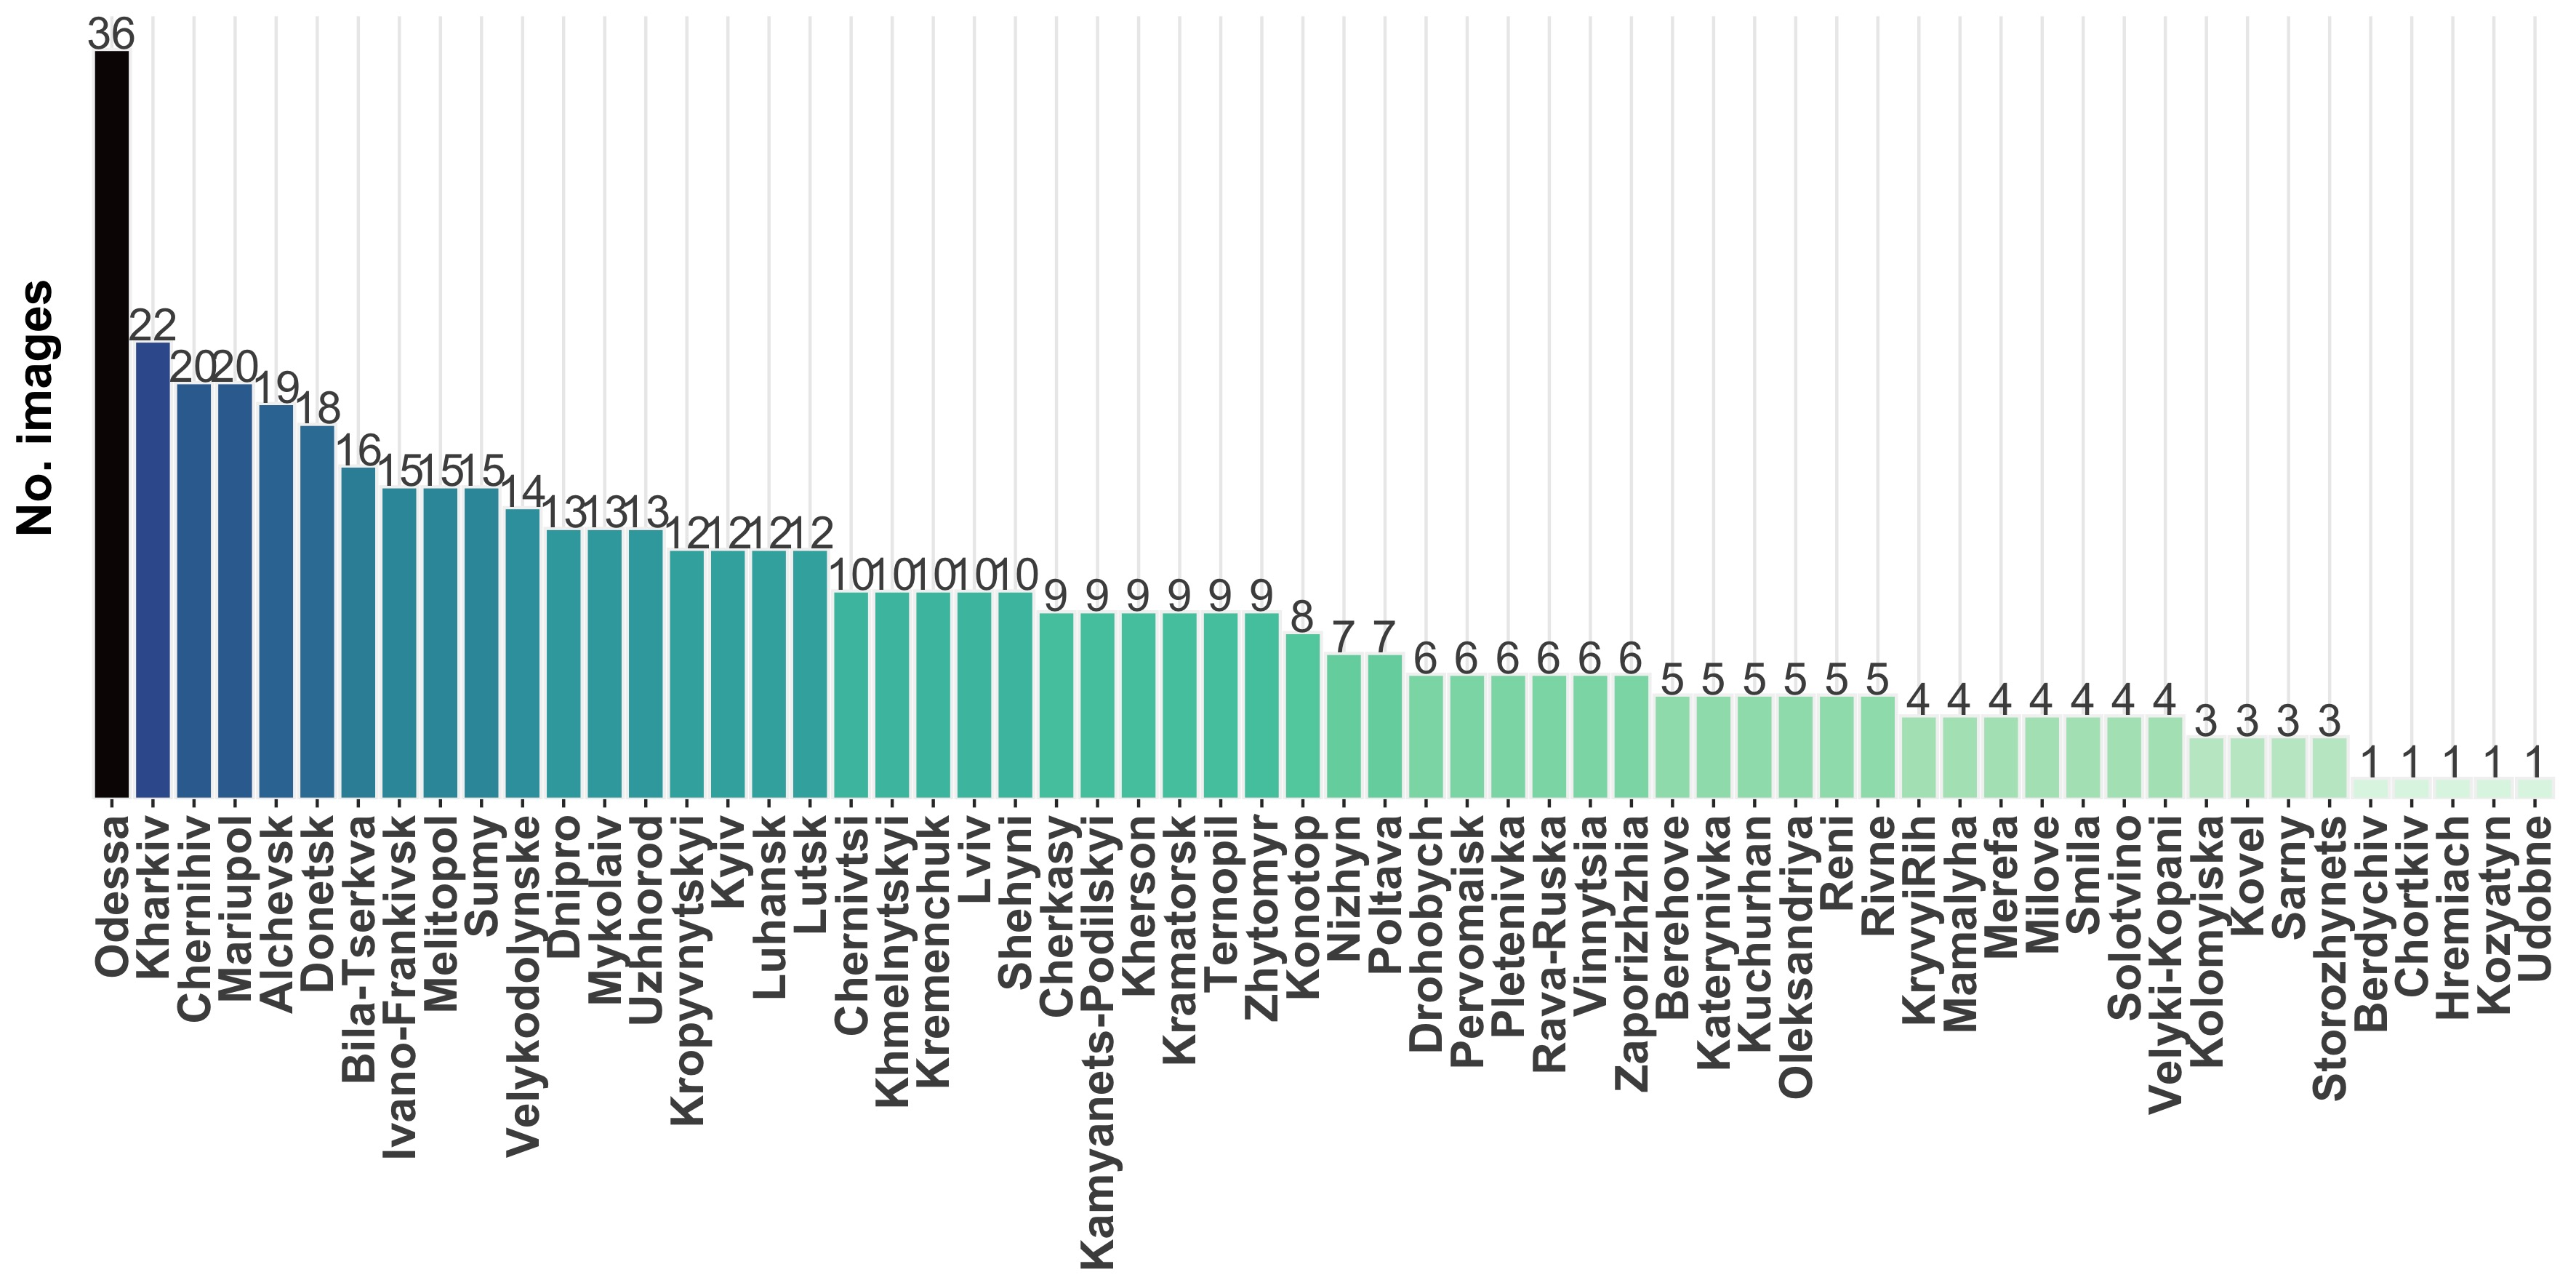
\includegraphics[width=\textwidth]{Figures/No_images_per_city.jpg}
\end{center}
\caption{Number of satellite images per city after the data post-processing pipeline (n =  534 images).}
\label{figSM_Nimages}
\end{figure}


% Data availability over time
%%%%%%%%%%%%%%%%%%%%%%%%%%%%%%
\begin{figure}[htbp]
\begin{center}
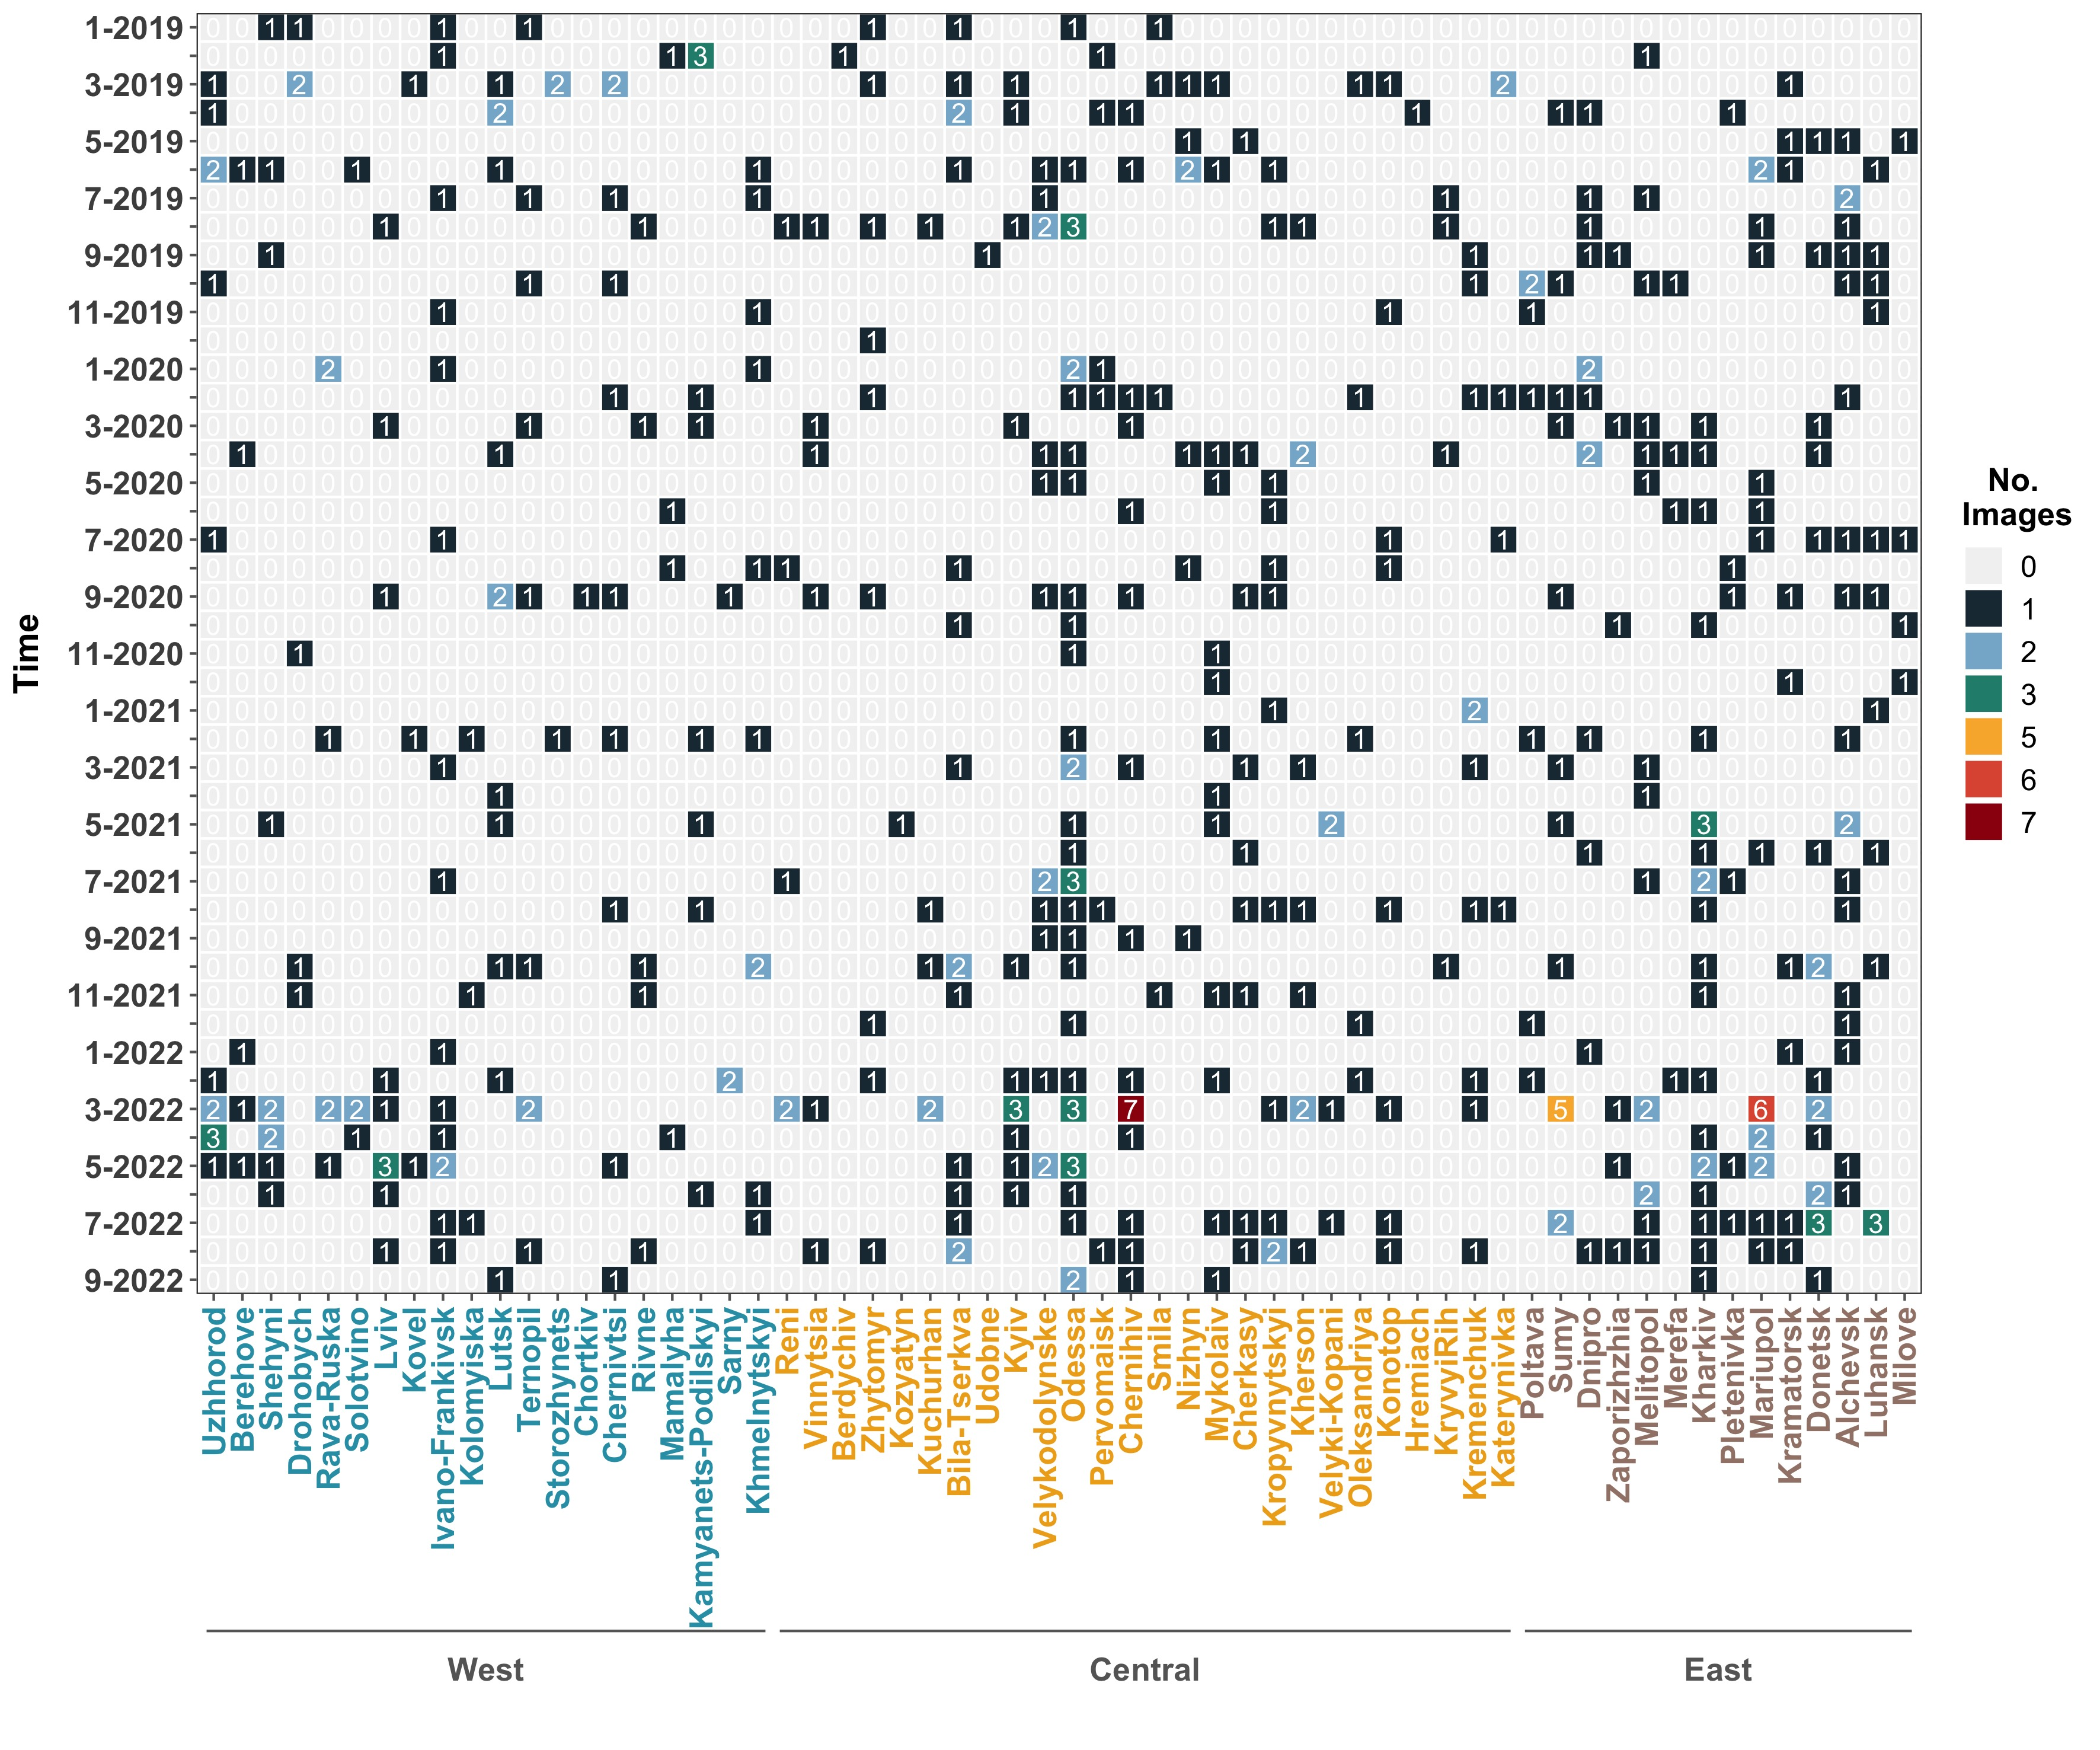
\includegraphics[scale = 0.10]{Figures/No_images_per_time.jpg}
\end{center}
\caption{Data availability across space and time after the post-processing pipeline (n =  534 images), with cities arranged from West to East. The color scale reflects the number of images per month, with warmer colors representing cases with larger number of images. Light-gray colored tiles denote months where no imagery were available.}
\label{figSM_DatAvail}
\end{figure}


% Imagery effect on car detection
%%%%%%%%%%%%%%%%%%%%%%%%%%%%%%%%%%

%%% Image resolution
\begin{figure}[htbp]
\begin{center}
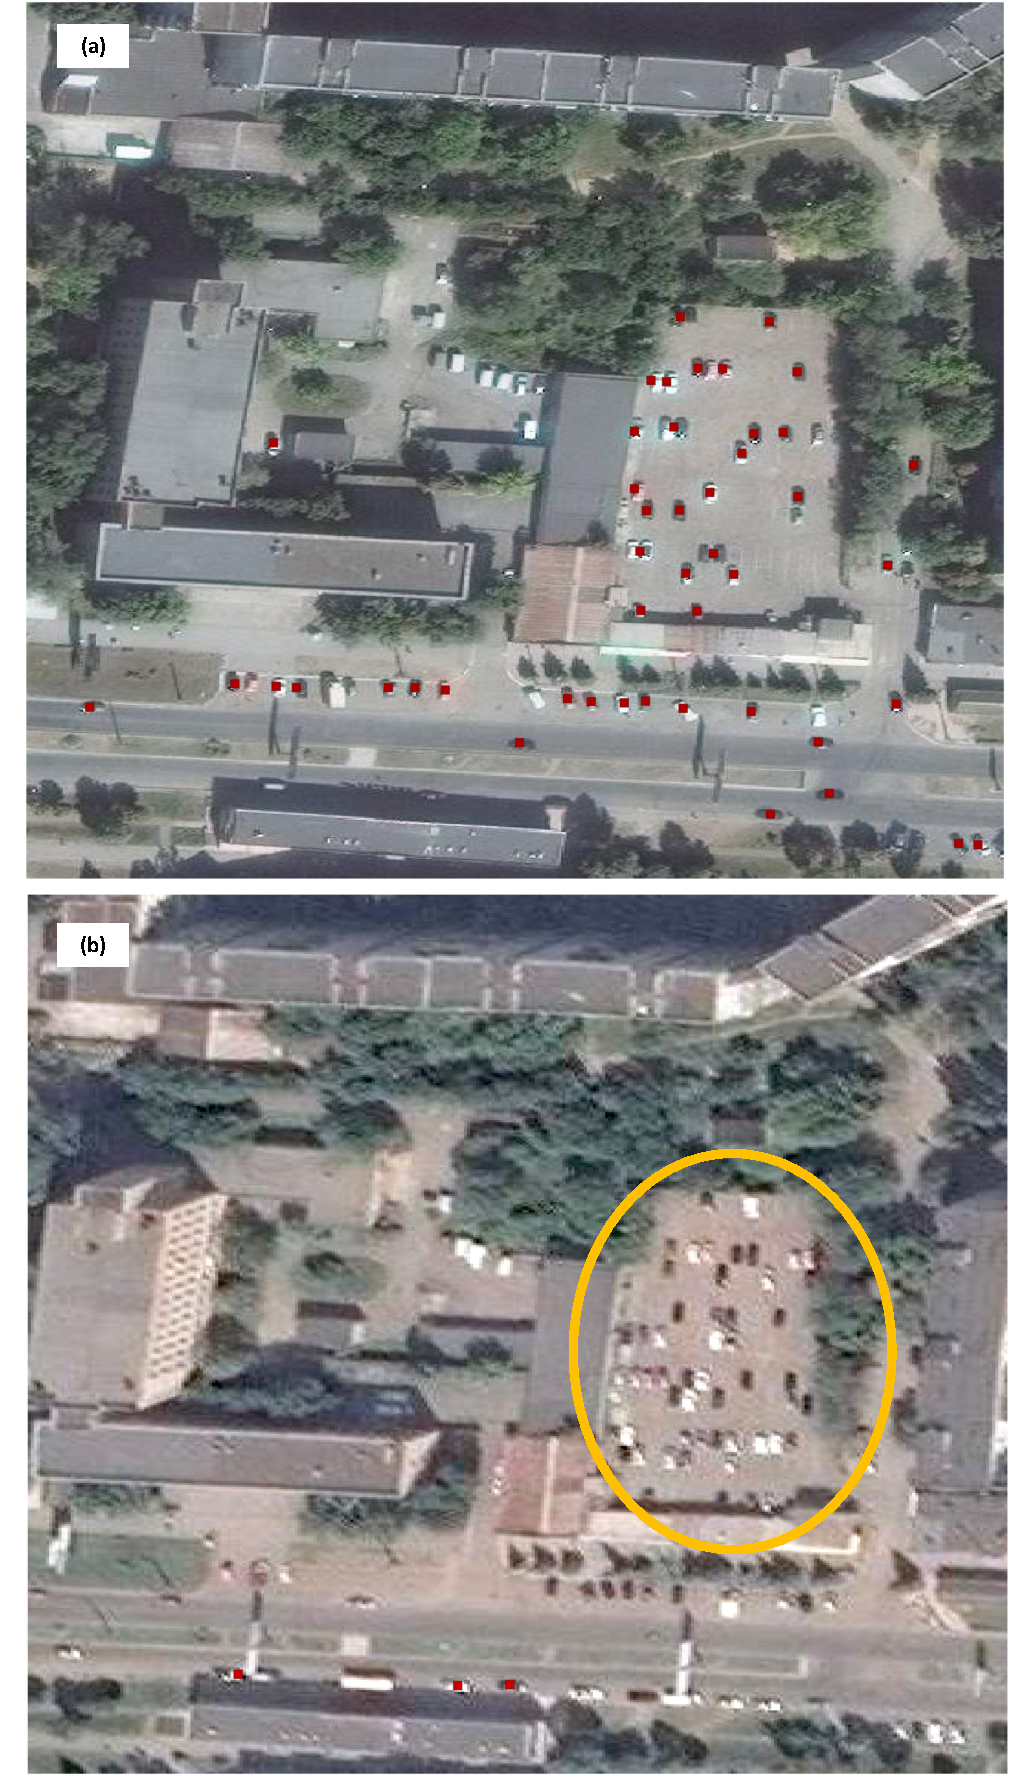
\includegraphics[scale = 0.5]{Figures/Image_Resolution.pdf}
\end{center}
\caption{Illustrative example from Alchevsk city on the effect of image resolution on car detection (marked as red squares in the images). The two panels shows a parking lot in front of a post office, whereby the Convolutional Neural Network (CNN) model detects visibly more cars in the higher-resolution image (0.3 m GSD; panel (a)) than in the lower-resolution image (0.5 m GSD; panel (b)). Note that both images were taken on similar time and dates (a = 12.09.2019 08:55 UTC, b = 24.08.2019 08:22 UTC), as well as had similar imagery features:  off-Nadir angle (a = 17.56\textdegree, b = 24.14\textdegree), sun elevation (a = 45.58\textdegree, b = 50.42\textdegree). The orange circle in panel (b) highlights the area where cars remained largely undetected. Satellite images \copyright ~2019--2023 Maxar Technologies.
}
\label{figSM_ImageResolution}
\end{figure}


%%% Snow effect
\begin{figure}[htbp]
\begin{center}
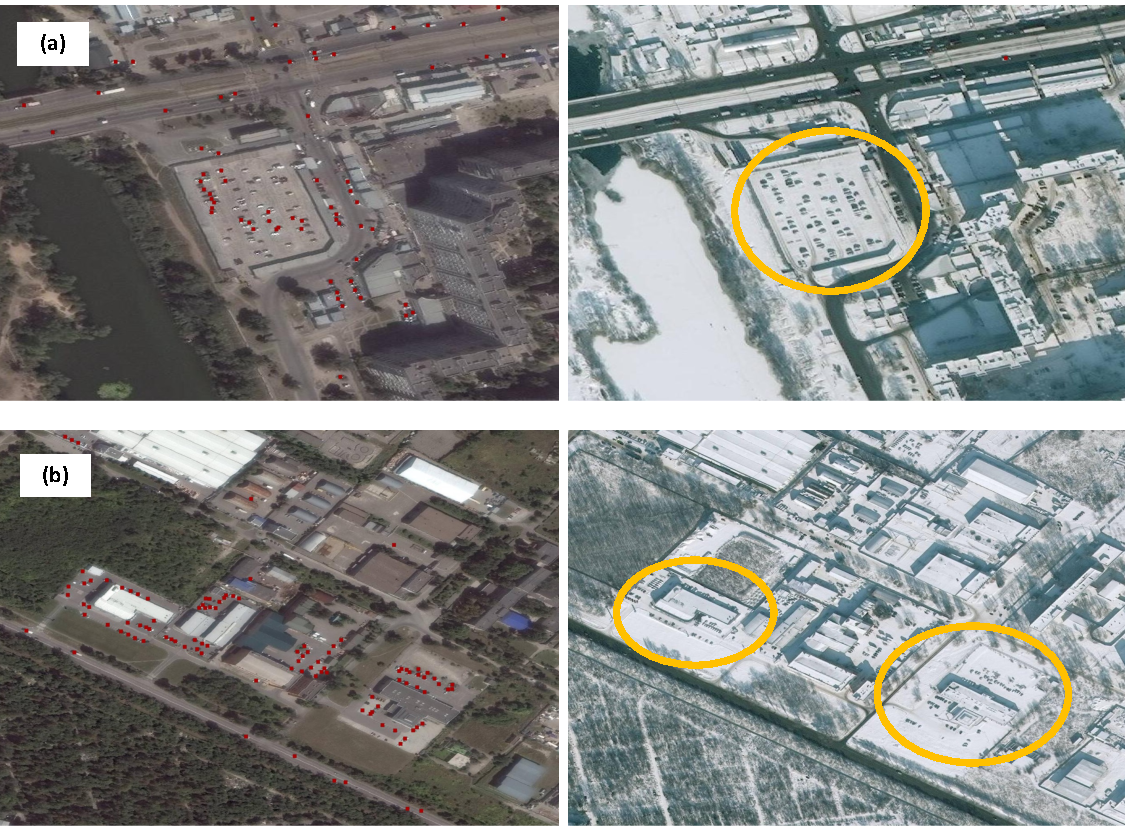
\includegraphics[width=\textwidth]{Figures/SnowEffect_final.pdf}
\end{center}
\caption{Illustrative example from Dnipro city to show the effect of snow on the detectability of cars. Both panels highlight two distinct commercial areas (a, b), with left and right panels showing the detected cars (red squares) on a summer and winter day, respectively. In the presence of snow (right panels), cars covered by snow remained undetected due to the reduced contrast. The orange circles in the right-side panels highlights the areas where cars remained largely undetected. Satellite images \copyright ~2019--2023 Maxar Technologies.
}
\label{figSM_SnowEffect}
\end{figure}


%%% off-Nadir 
\begin{figure}[htbp]
\begin{center}
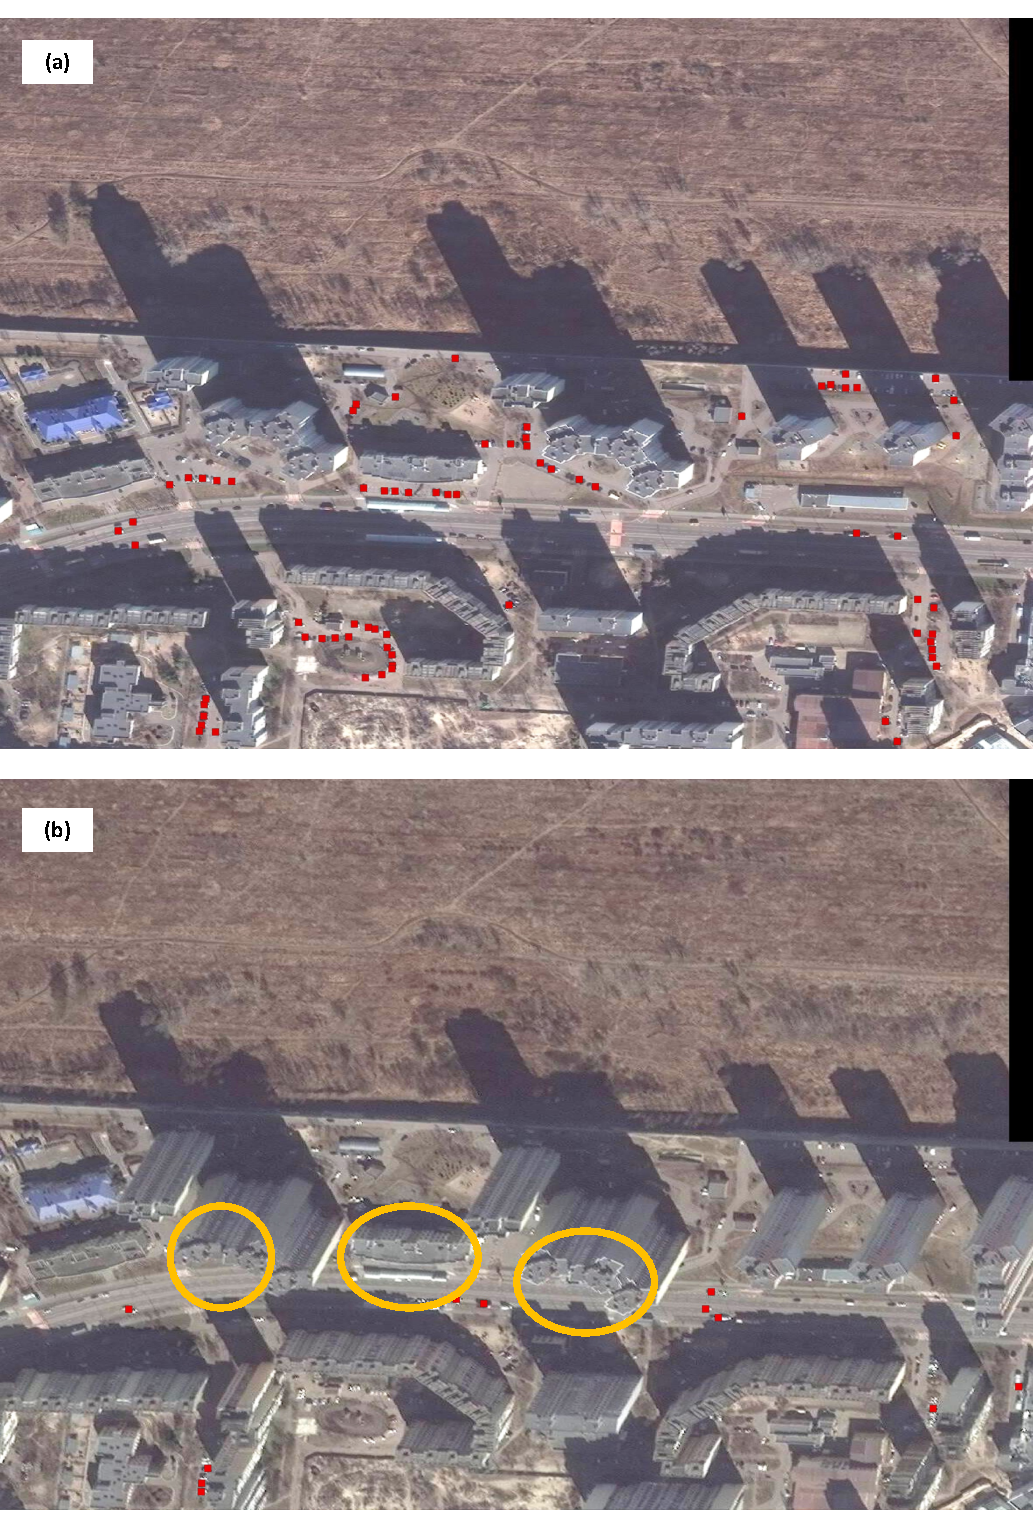
\includegraphics[scale = 0.5]{Figures/OffNadir_final.pdf}
\end{center}
\caption{Snapshots from the same residential area in Kiev city to illustrate the off-Nadir angle effect on the detectability of cars (a = 10.84\textdegree, b = 37.08\textdegree).
The two panels clearly show that more cars are detected at smaller off-Nadir angles (a). At larger viewing angles (b), the buildings tend to occlude other important infrastructure such as roads and parking lots and obfuscate the circulating cars, thus reducing the detectability.  Note that both images were taken on similar time of the day (a = 09:06 UTC, b = 09:05 UTC), while also had similar imagery features: sun elevation angle (a = 30.17\textdegree , b = 37.58\textdegree), image resolution (a = b = 0.5 m GSD). The orange circles in the lower panel highlights the areas where cars remained largely undetected. Satellite images \copyright ~2019--2023 Maxar Technologies.
}
\label{figSM_OffNadir}
\end{figure}


%%% Sun elevation 
\begin{figure}[htbp]
\begin{center}
\includegraphics[scale = 0.5]{Figures/SunElevation_final.pdf}
\end{center}
\caption{Snapshots from the same commercial area in Dnipro city to illustrate the effect of sun elevation angle on the detectability of cars (a = 58.68\textdegree, b = 17.96\textdegree). At greater angles, the shadows created by the buildings are reduced, resulting in greater discernability of the circulating cars as in Panel (a) whereas Panel (b) shows that fewer cars are detected at smaller angles. Note that both images were taken on similar time of the day (a = 08:36 UTC, b = 08:41 UTC), while also had similar imagery features:  off-Nadir angle (a = 17.81\textdegree , b = 12.69\textdegree), image resolution (a = b = 0.4 m GSD). The orange circles in the lower panel highlights the areas where cars remained largely undetected. Satellite images \copyright ~2019--2023 Maxar Technologies.
}
\label{figSM_SunElevation}
\end{figure}



% GLM diagnostics
%%%%%%%%%%%%%%%%%%%
\begin{figure}[htbp]
\begin{center}
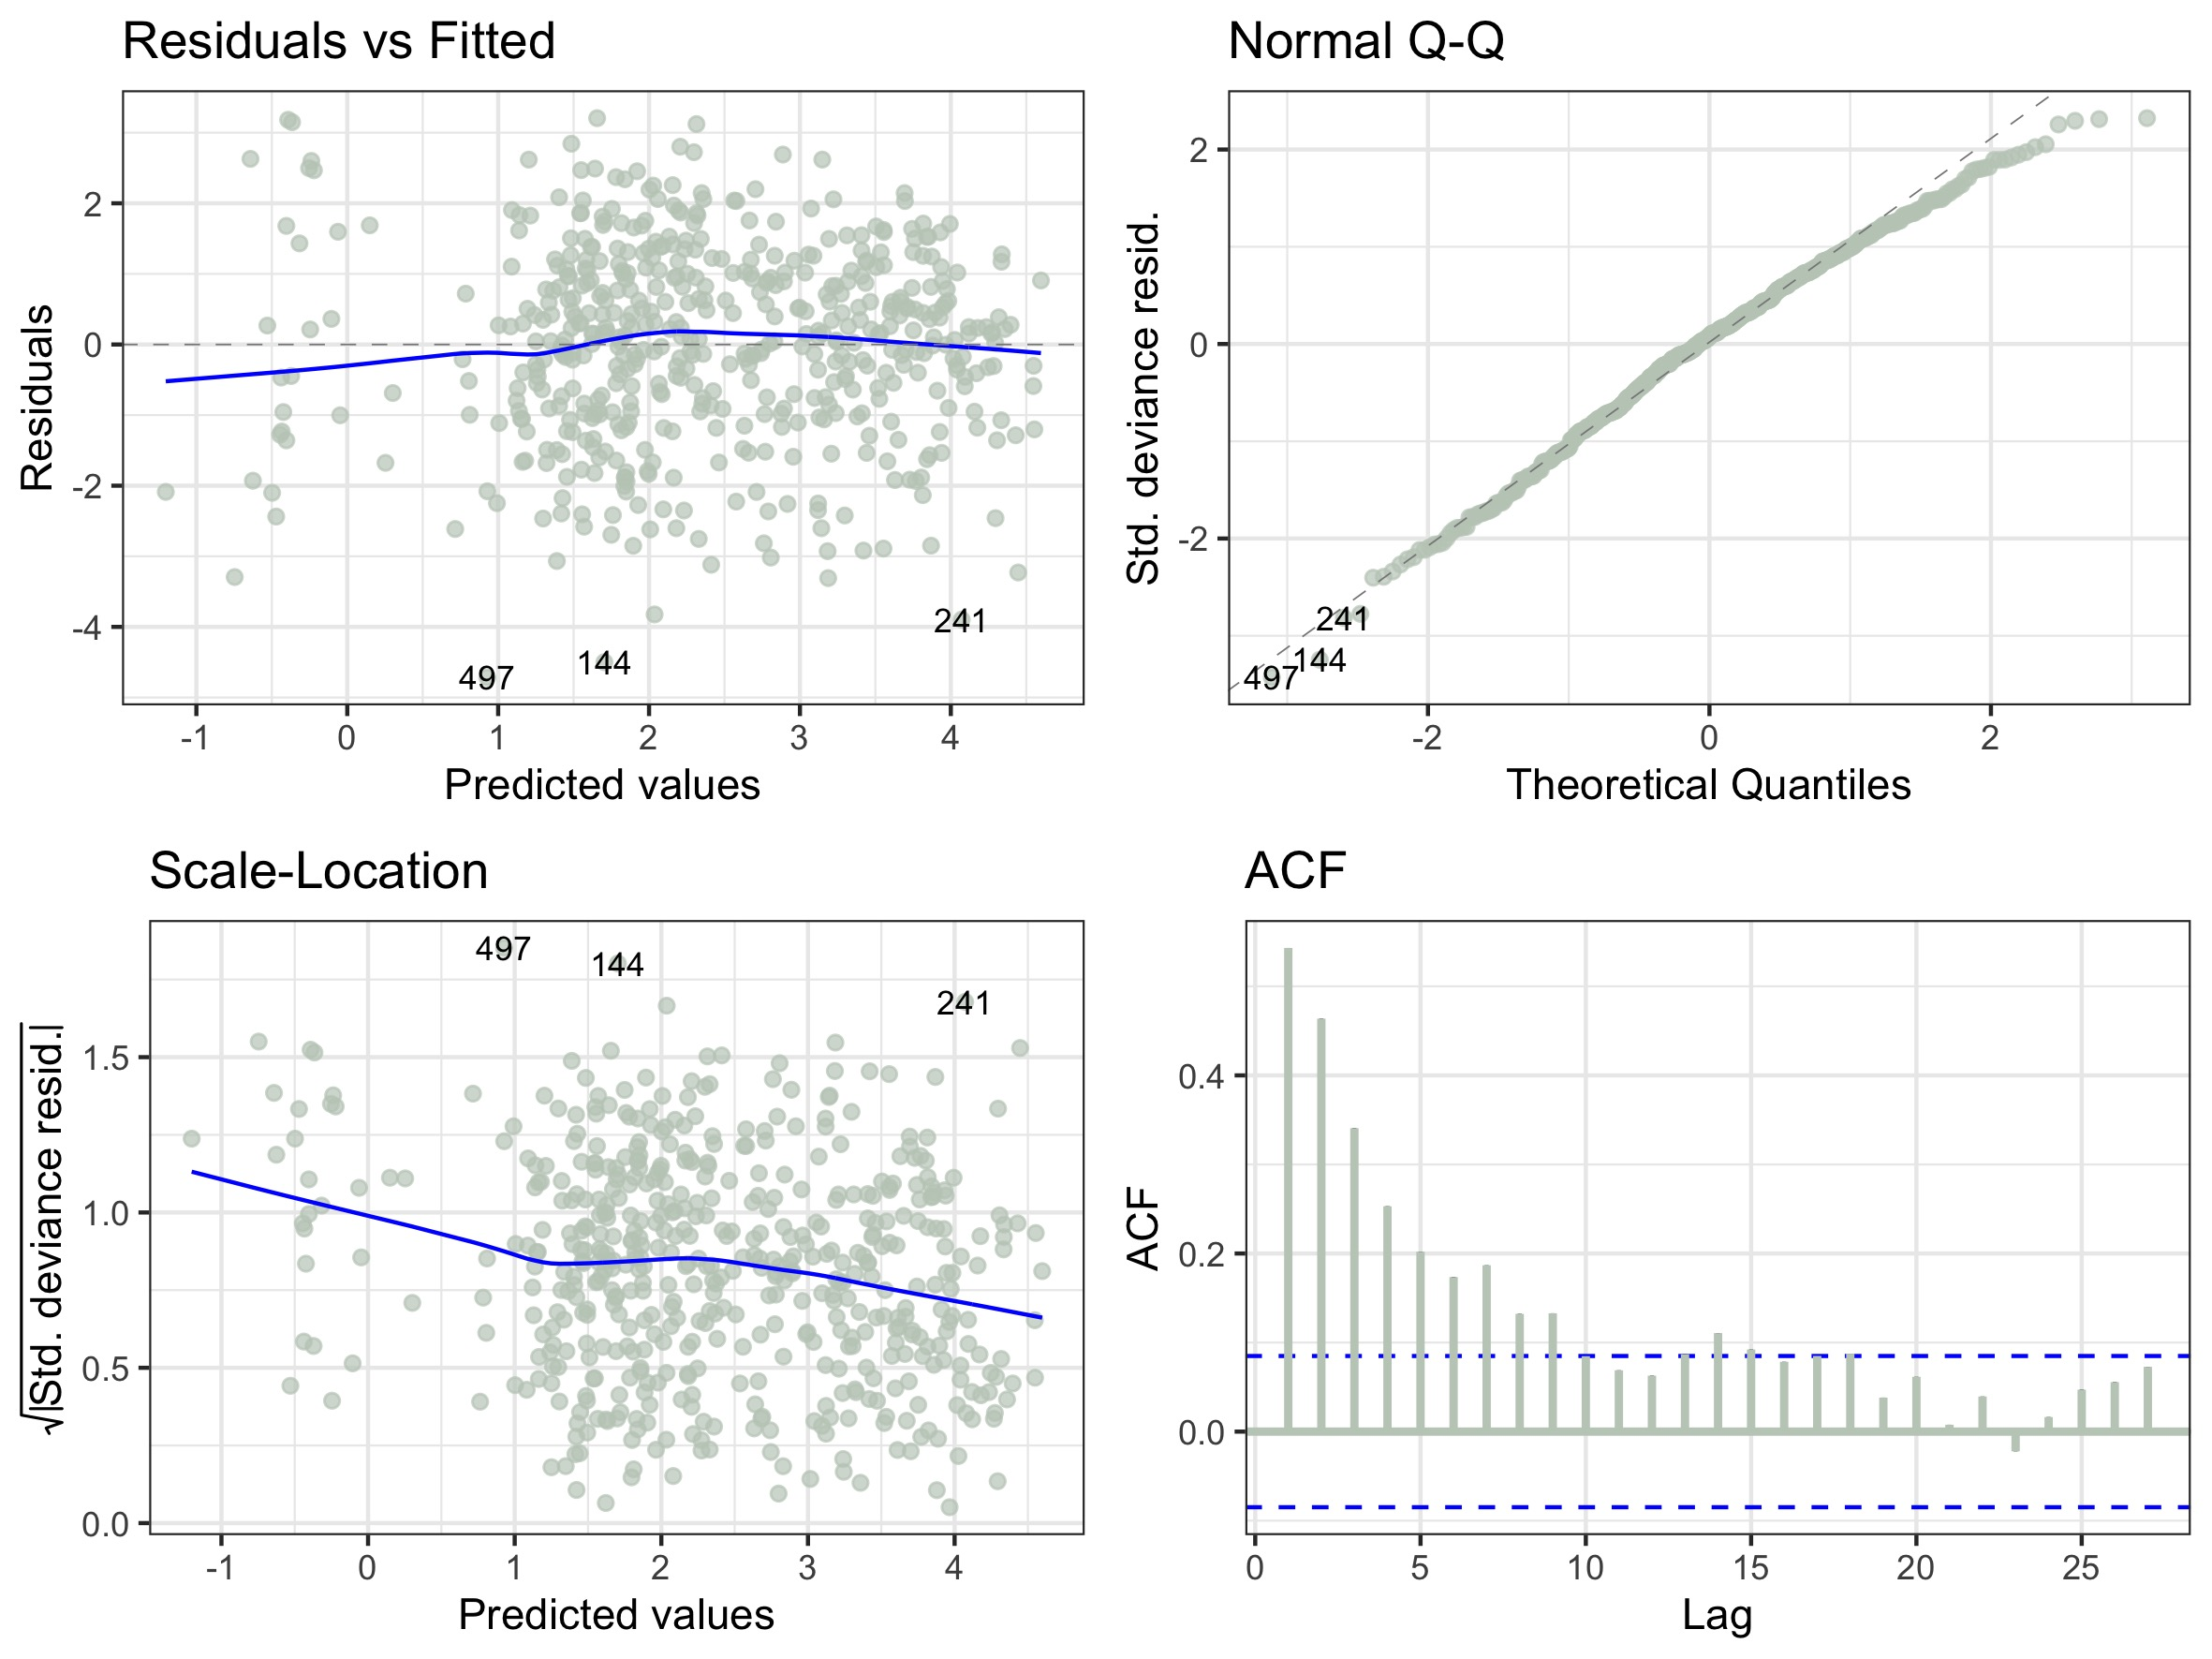
\includegraphics[width=\textwidth]{Figures/GLM_diagnostics.jpg}
\end{center}
\caption{Visual diagnostics of the Generalized Linear Model (GLM) applied to evaluate the effect of satellite imagery-related covariates on car detection.}
\label{figSM_Diagnostics}
\end{figure}


% Confidence threshold experiment
%%%%%%%%%%%%%%%%%%%%%%%%%%%%%%%%%%
\begin{figure}[htbp]
\begin{center}
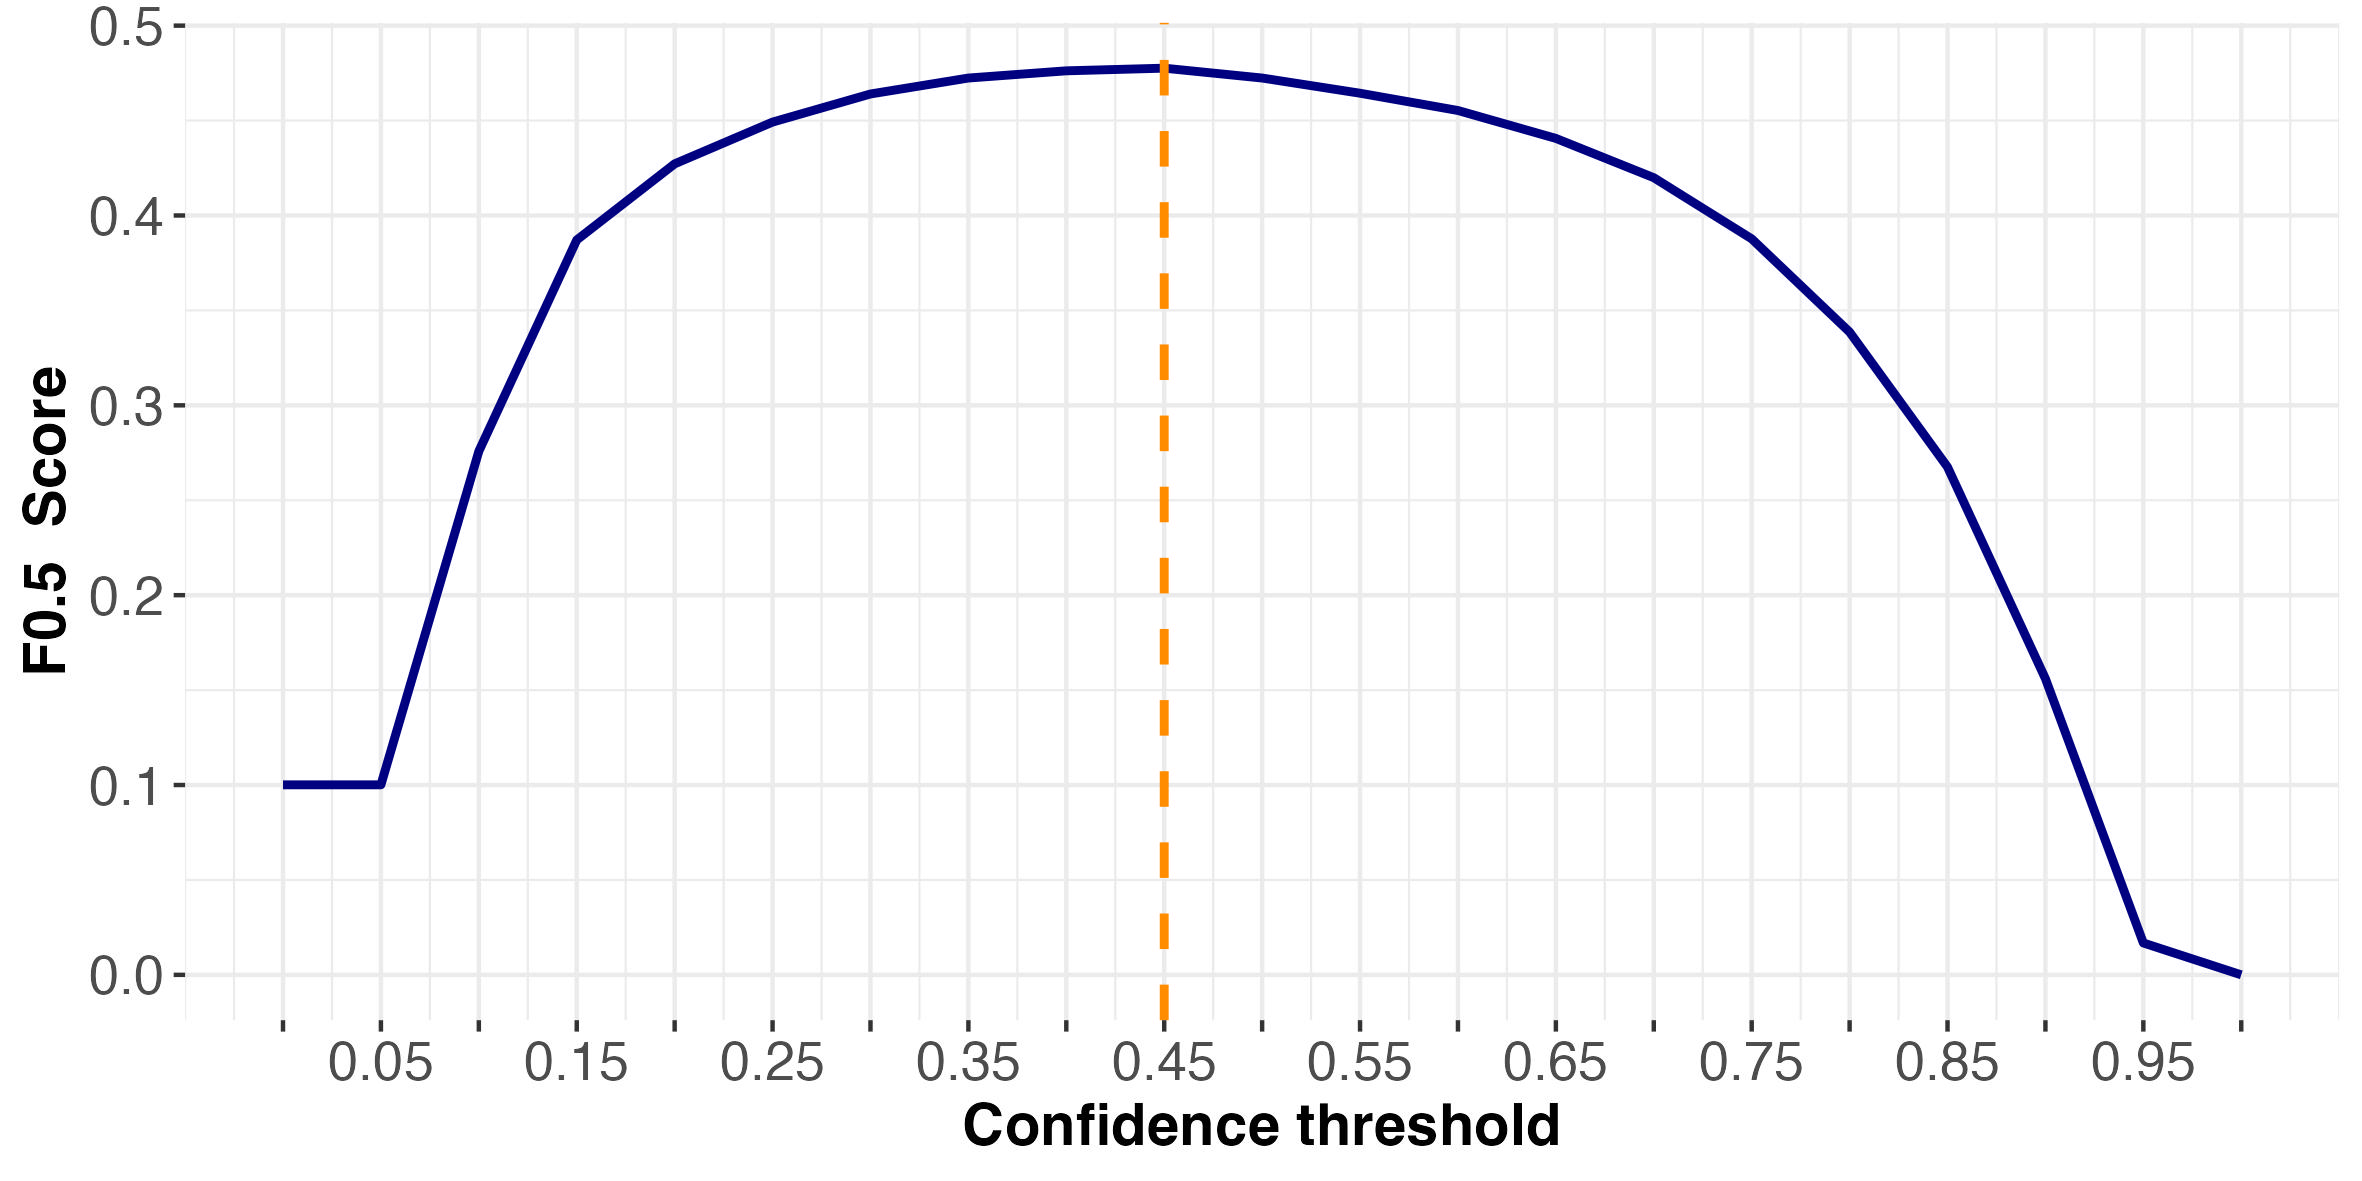
\includegraphics[width=\textwidth]{Figures/Confidence_threshold_experiment.jpg}
\end{center}
\caption{Results from the sensitivity test to evaluate the optimal confidence threshold to detect cars from the satellite images. A F-beta score of 0.5 gives more weight to precision than recall, minimizing as such the detection of false-positives.}
\label{figSM_Threshold}
\end{figure}


% False-positives
%%%%%%%%%%%%%%%%%%%
\begin{figure}[h!]
\begin{center}
\includegraphics[width=0.9\textwidth]{Figures/False_positives_final.pdf}
\end{center}
\caption{Satellite images showing  false car detections marked by the red squares. The three panels illustrate three distinct types of false-positives: (a) on air-conditioners fixed on top of commercial buildings in Odessa, b) on the Pivdennyi Buh River in Mykolaiv, and (c) on crop fields in Luhansk. Satellite images \copyright ~2019--2023 Maxar Technologies}
\label{figSM_FalsePositives}
\end{figure}

% Population coverage
%%%%%%%%%%%%%%%%%%%%%%%
\begin{figure}[h!]
\begin{center}
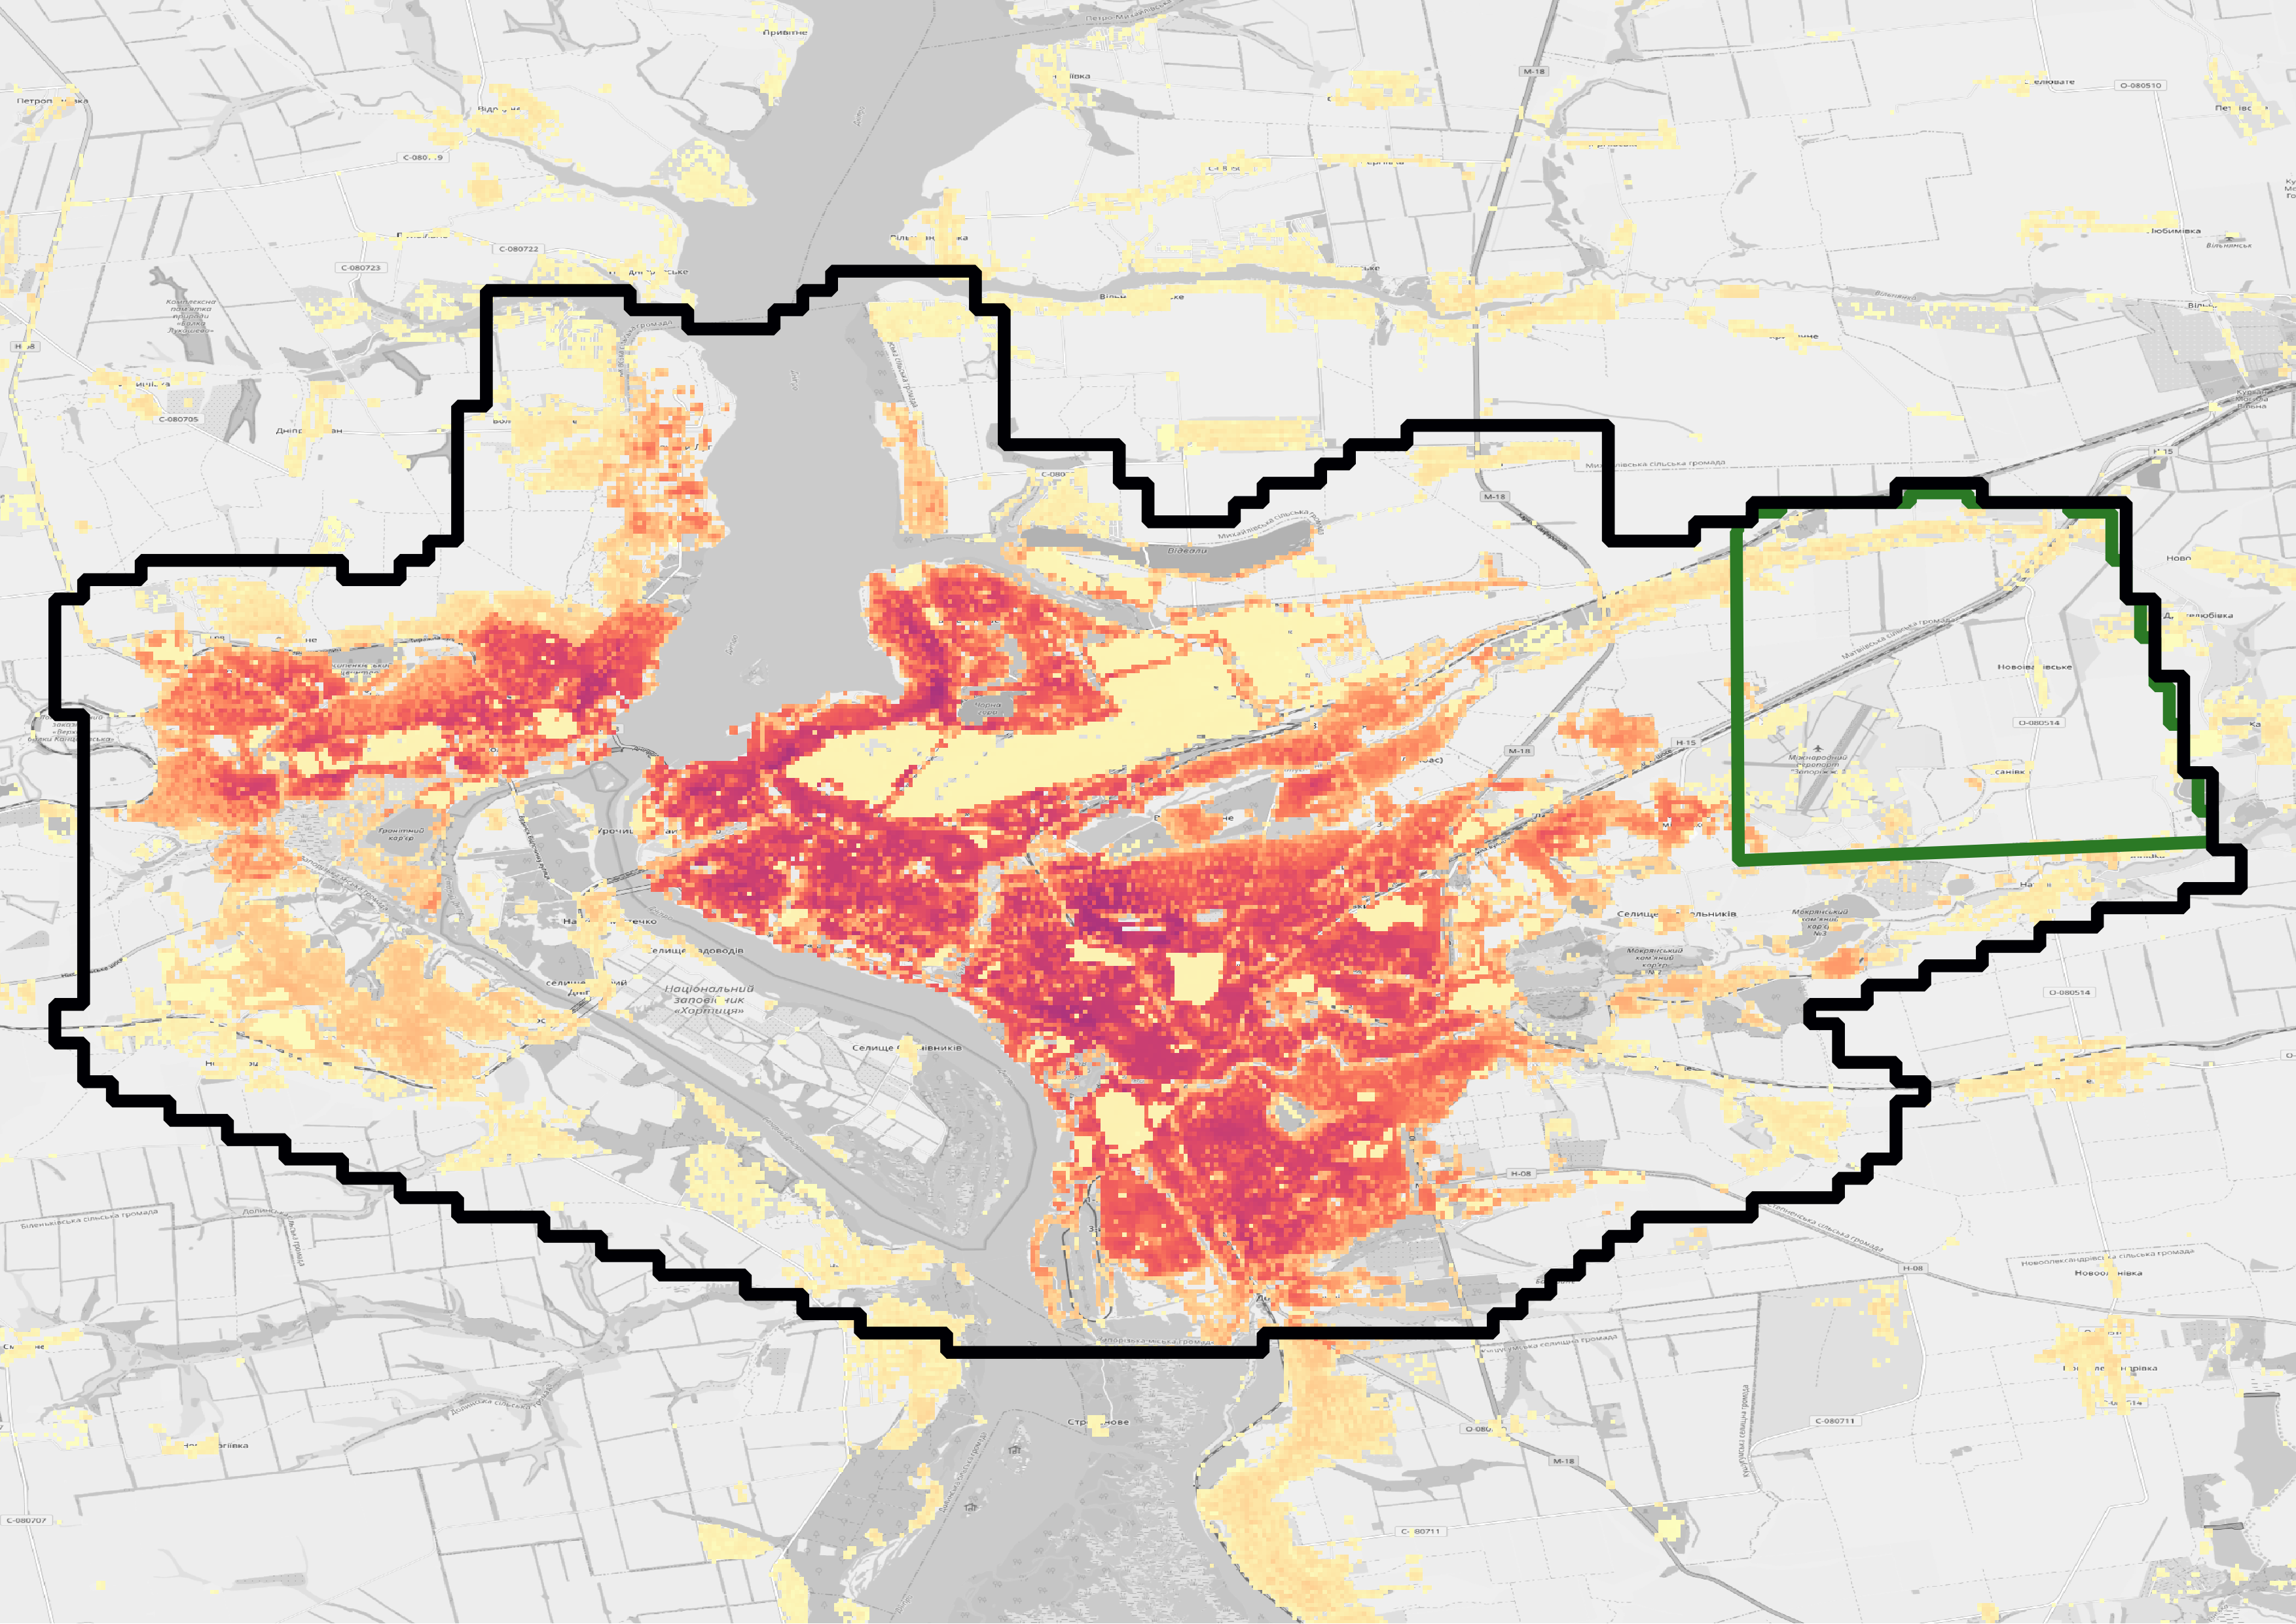
\includegraphics[width = \textwidth]{Figures/SM_Pop_coverage.png}
\end{center}
\caption{Population distribution for the city of Zaporizhzhia overlaid to the spatial extent of two different satellite images. The black and green line refers to the images taken in 19.03.2020 and 23.01.2020, respectively. While the first image covers the full extent of the Area of Interest (AOI), hence 100\% of the population distribution, the second image covers less than 50\% of the AOI which is located on an area that represents less than 1\% of the city's population. }
\label{SM_pop_coverage}
\end{figure}


% Cloud and haze obstructions 
%%%%%%%%%%%%%%%%%%%%%%%%%%%%%%



% Pop~car scatterplot
%%%%%%%%%%%%%%%%%%%%%

%%% fig 1
\begin{figure}[h!]
\begin{center}
\includegraphics[width=0.95\textwidth]{Figures/popcar_S1.jpg}
\end{center}
\caption{Relationship between the gridded average number of people and cars during the reference year (2019) for the selected Ukrainian cities. Each circle represents a unique spatial grid cell (1 x 1 km), with its size reflecting the population/car ratio. The orange smoothed function highlights the trend line from the GAM model bounded by its 95\% confidence interval.}
\label{figSM_PopCar_01}
\end{figure}


%%% fig 2
\begin{figure}[h!]
\begin{center}
\includegraphics[width=0.95\textwidth]{Figures/popcar_S2.jpg}
\end{center}
\caption{Cont. - Relationship between the gridded average number of people and cars during the reference year (2019) for the selected Ukrainian cities. Each circle represents a unique spatial grid cell (1 x 1 km), with its size reflecting the population/car ratio. The orange smoothed function highlights the trend line from the GAM model bounded by its 95\% confidence interval.}
\label{figSM_PopCar_02}
\end{figure}


%%% fig 3
\begin{figure}[h!]
\begin{center}
\includegraphics[width=0.95\textwidth]{Figures/popcar_S3.jpg}
\end{center}
\caption{Cont. - Relationship between the gridded average number of people and cars during the reference year (2019) for the selected Ukrainian cities. Each circle represents a unique spatial grid cell (1 x 1 km), with its size reflecting the population/car ratio. The orange smoothed function highlights the trend line from the GAM model bounded by its 95\% confidence interval.}
\label{figSM_PopCar_03}
\end{figure}


%%% fig 4
\begin{figure}[h!]
\begin{center}
\includegraphics[width=0.95\textwidth]{Figures/popcar_S4.jpg}
\end{center}
\caption{Cont. - Relationship between the gridded average number of people and cars during the reference year (2019) for the selected Ukrainian cities. Each circle represents a unique spatial grid cell (1 x 1 km), with its size reflecting the population/car ratio. The orange smoothed function highlights the trend line from the GAM model bounded by its 95\% confidence interval.}
\label{figSM_PopCar_04}
\end{figure}


%%% fig 5
\begin{figure}[h!]
\begin{center}
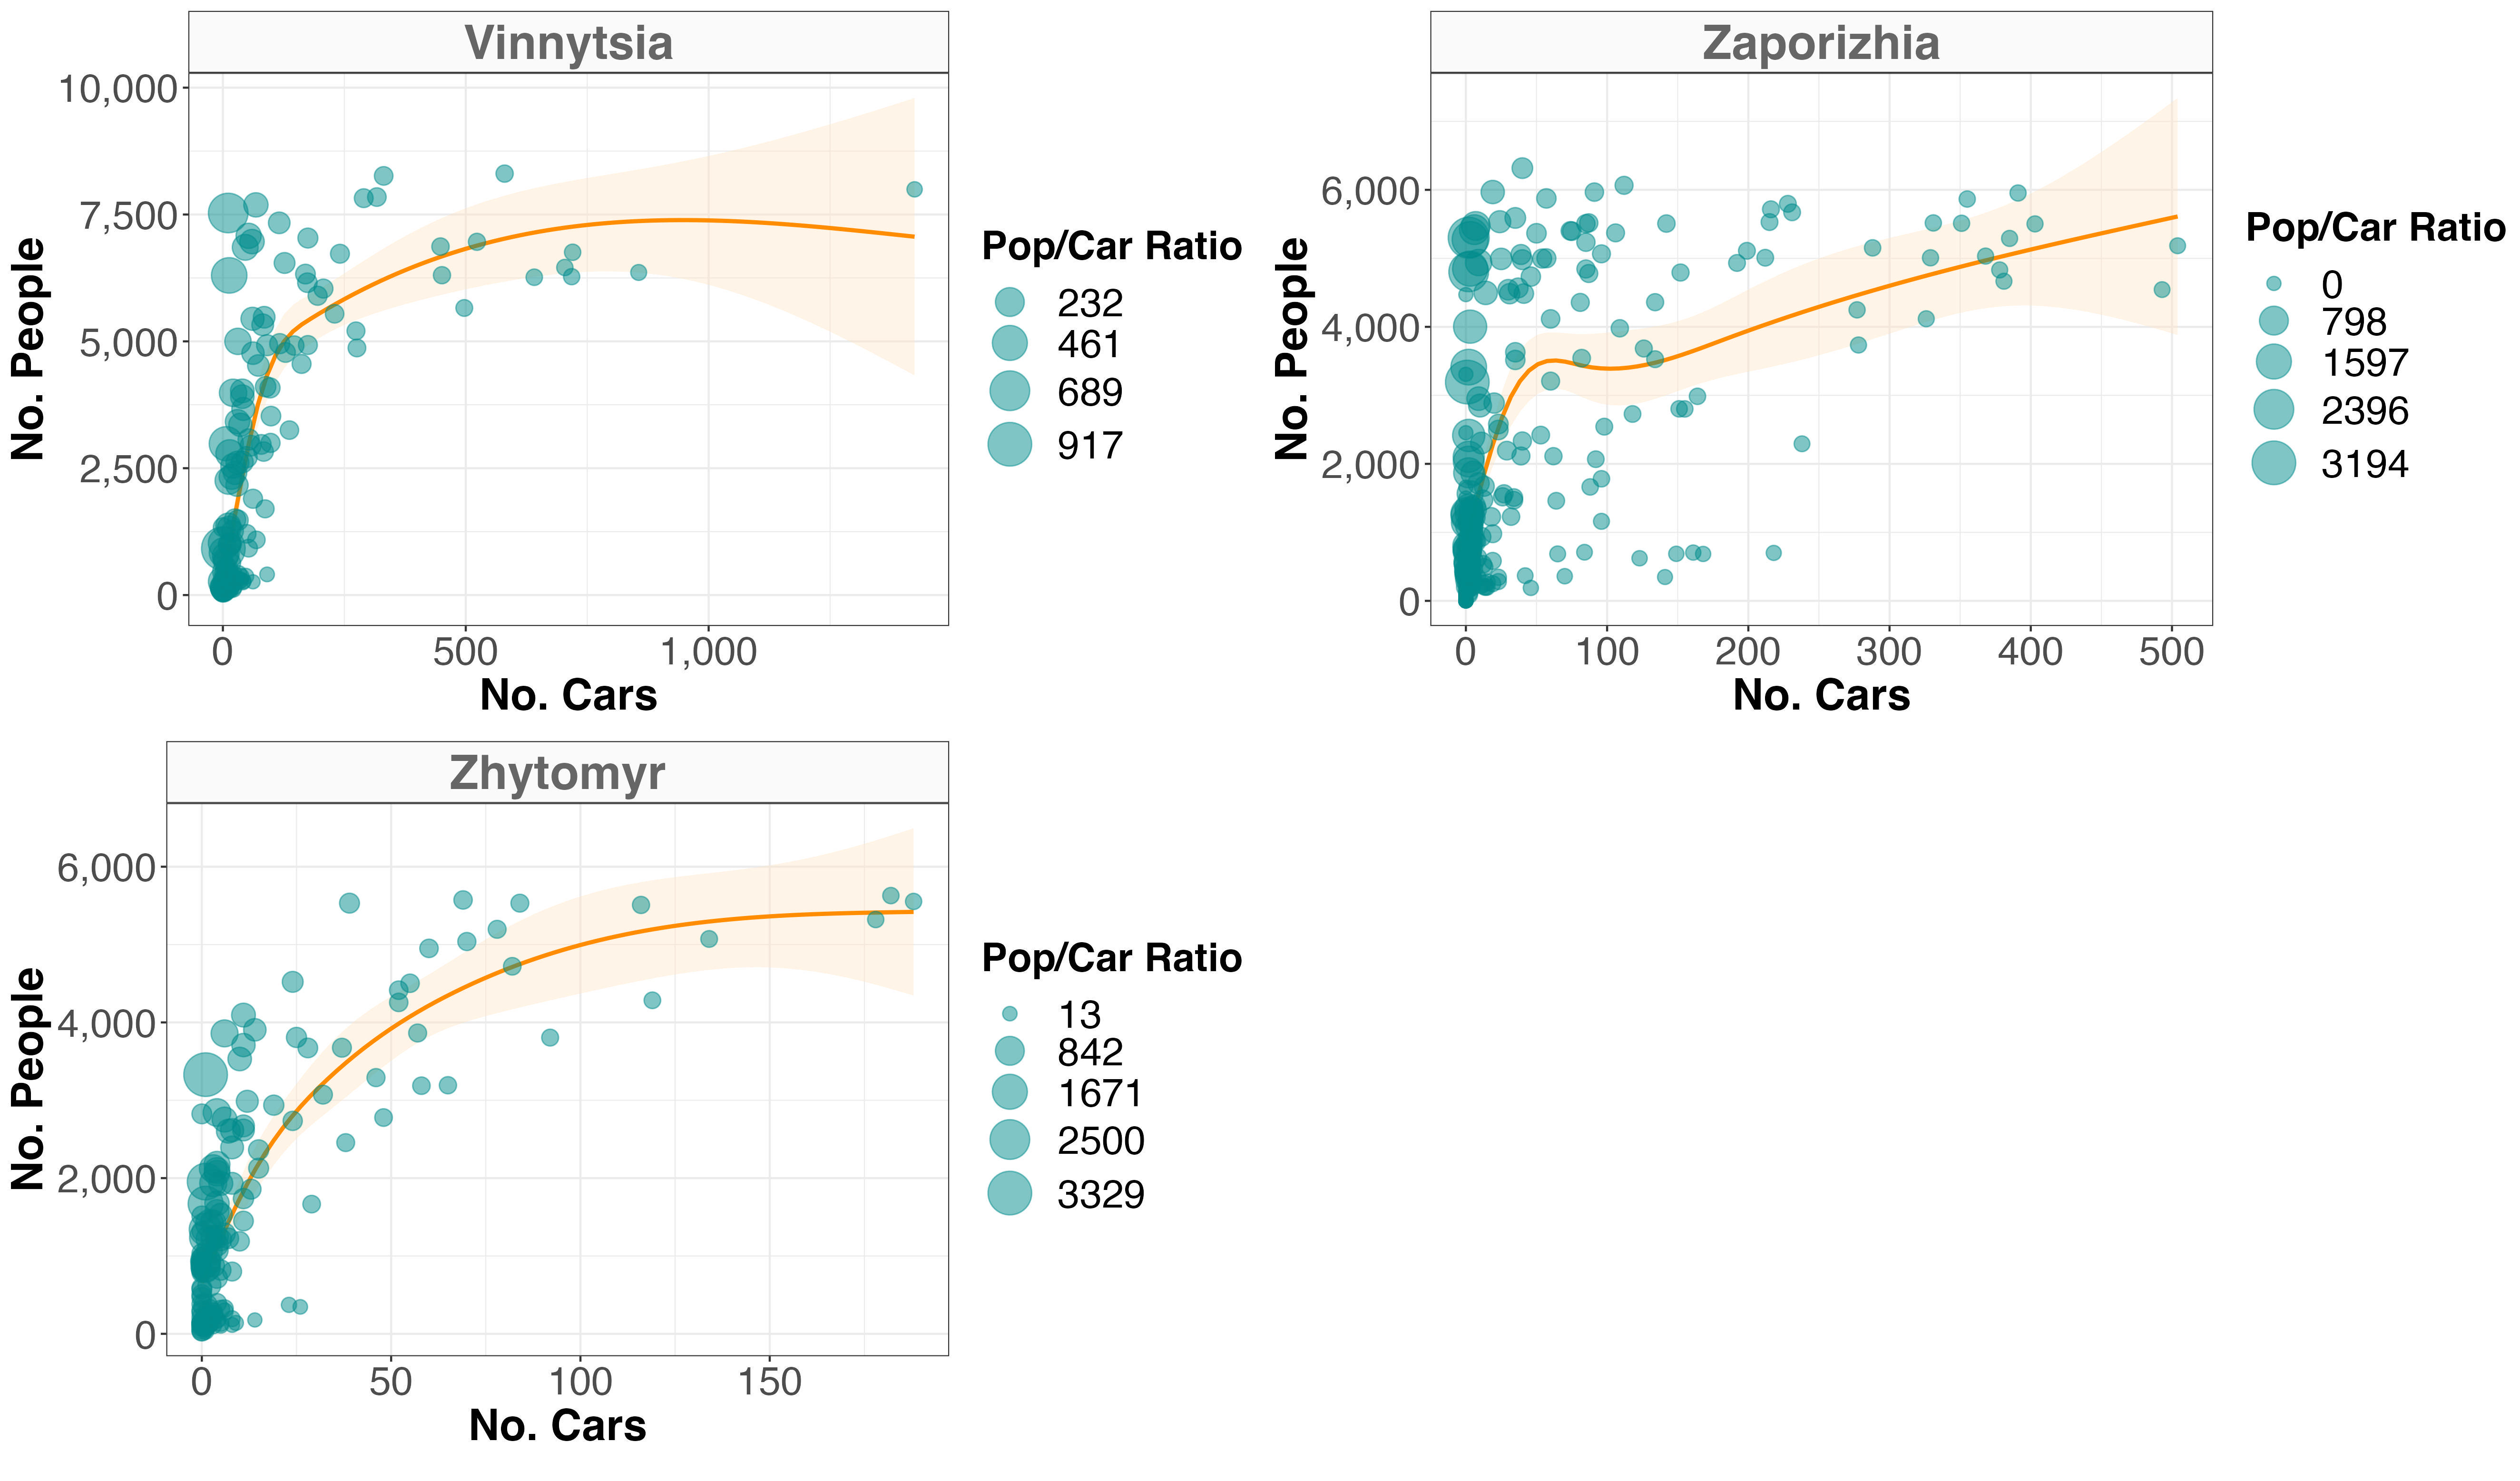
\includegraphics[width=0.95\textwidth]{Figures/popcar_S5.jpg}
\end{center}
\caption{Cont. - Relationship between the gridded average number of people and cars during the reference year (2019) for the selected Ukrainian cities. Each circle represents a unique spatial grid cell (1 x 1 km), with its size reflecting the population/car ratio. The orange smoothed function highlights the trend line from the GAM model bounded by its 95\% confidence interval.}
\label{figSM_PopCar_05}
\end{figure}


% IDP predictions - Barchart
%%%%%%%%%%%%%%%%%%%%%%%%%%%

%%% fig 1
\begin{figure}[h!]
\begin{center}
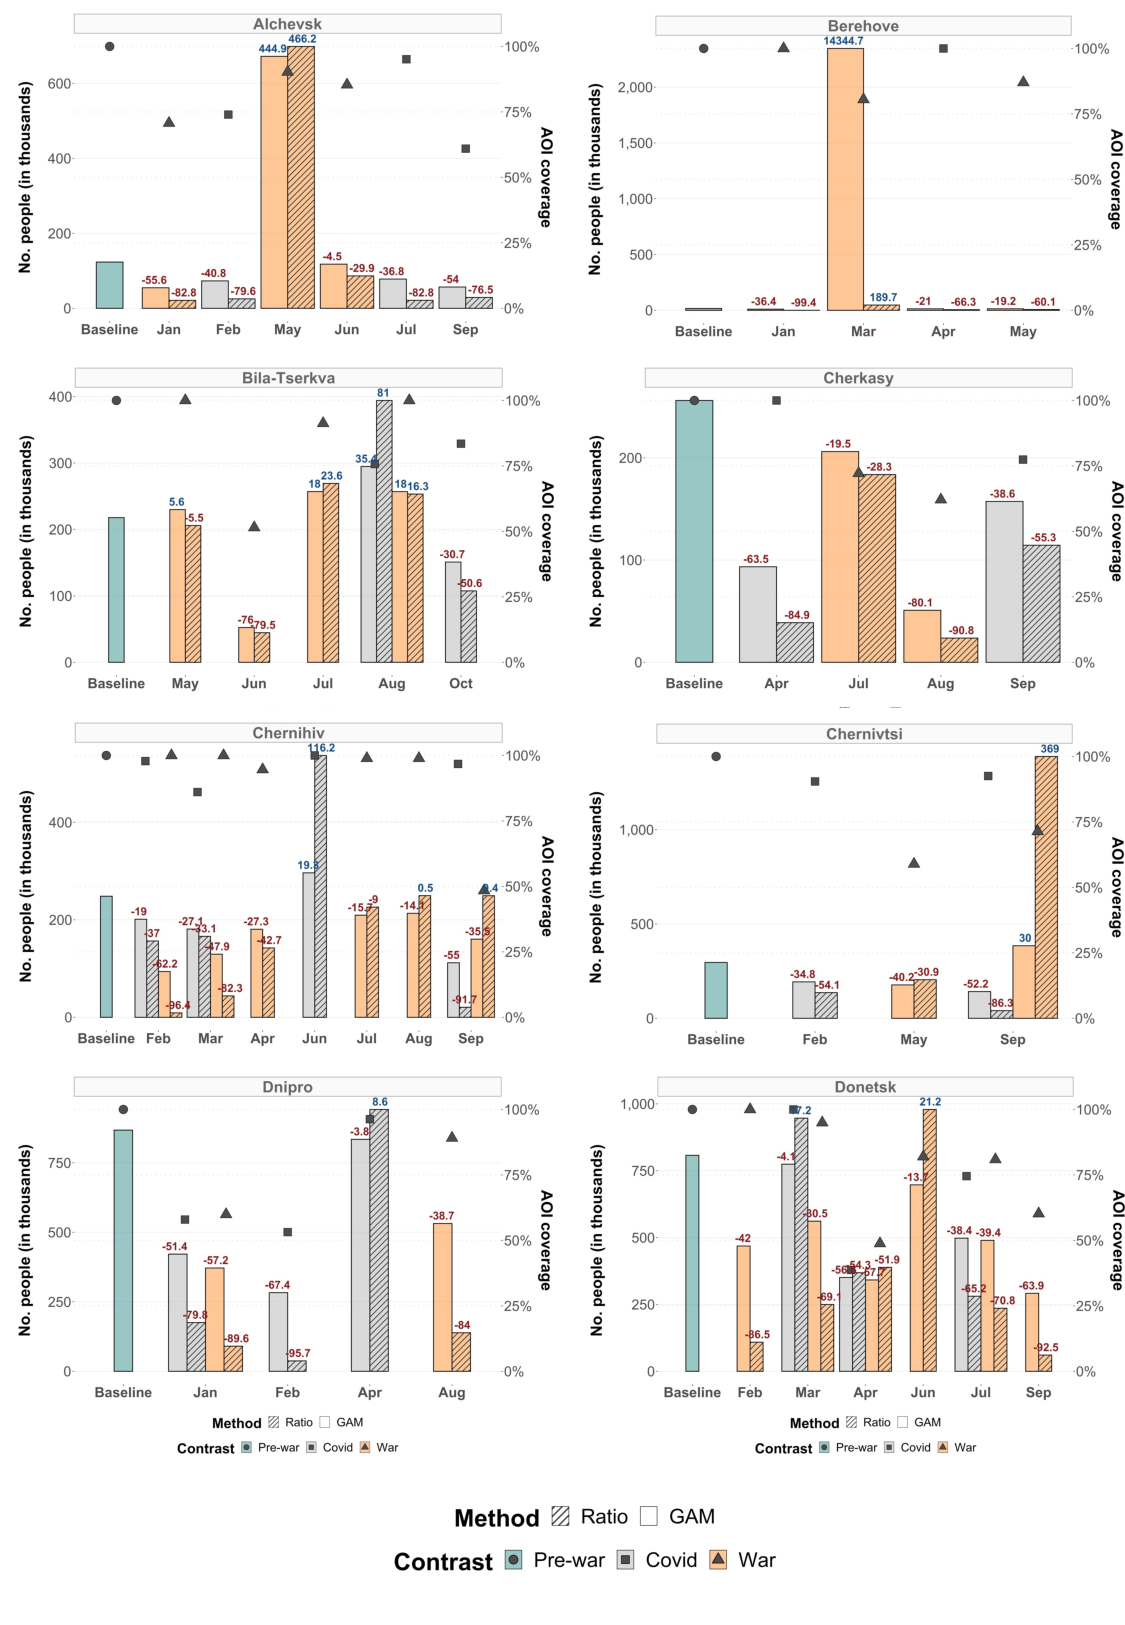
\includegraphics[scale = 0.6]{Figures/SM_IDP_pred_Fig1.pdf}
\end{center}
\caption{Predictions of internally displaced people across three different cities in Ukraine. The turquoise bar marks the pre-War population size (2019), from which relative change in population size has been derived for the applicable months in either 2020 (first COVID-19 year, gray bars) or 2022 (War year, orange bars). Numbers on top of each bar denote the relative population change (in \%), with colors reflecting either an increase (blue) or decrease (red). Dashed and plain bars distinguish the two tested prediction methods: linear ratio (dashed) and Generalized Additive Model (GAM, plain). Moreover, the overlaid symbols, related to the secondary y-axis, depict the percentage of area covered by the satellite images underlying a given month relative to the city's area of interest (AOI).}
\label{figSM_IDP_pred_Fig1}
\end{figure}

%%% fig 2
\begin{figure}[h!]
\begin{center}
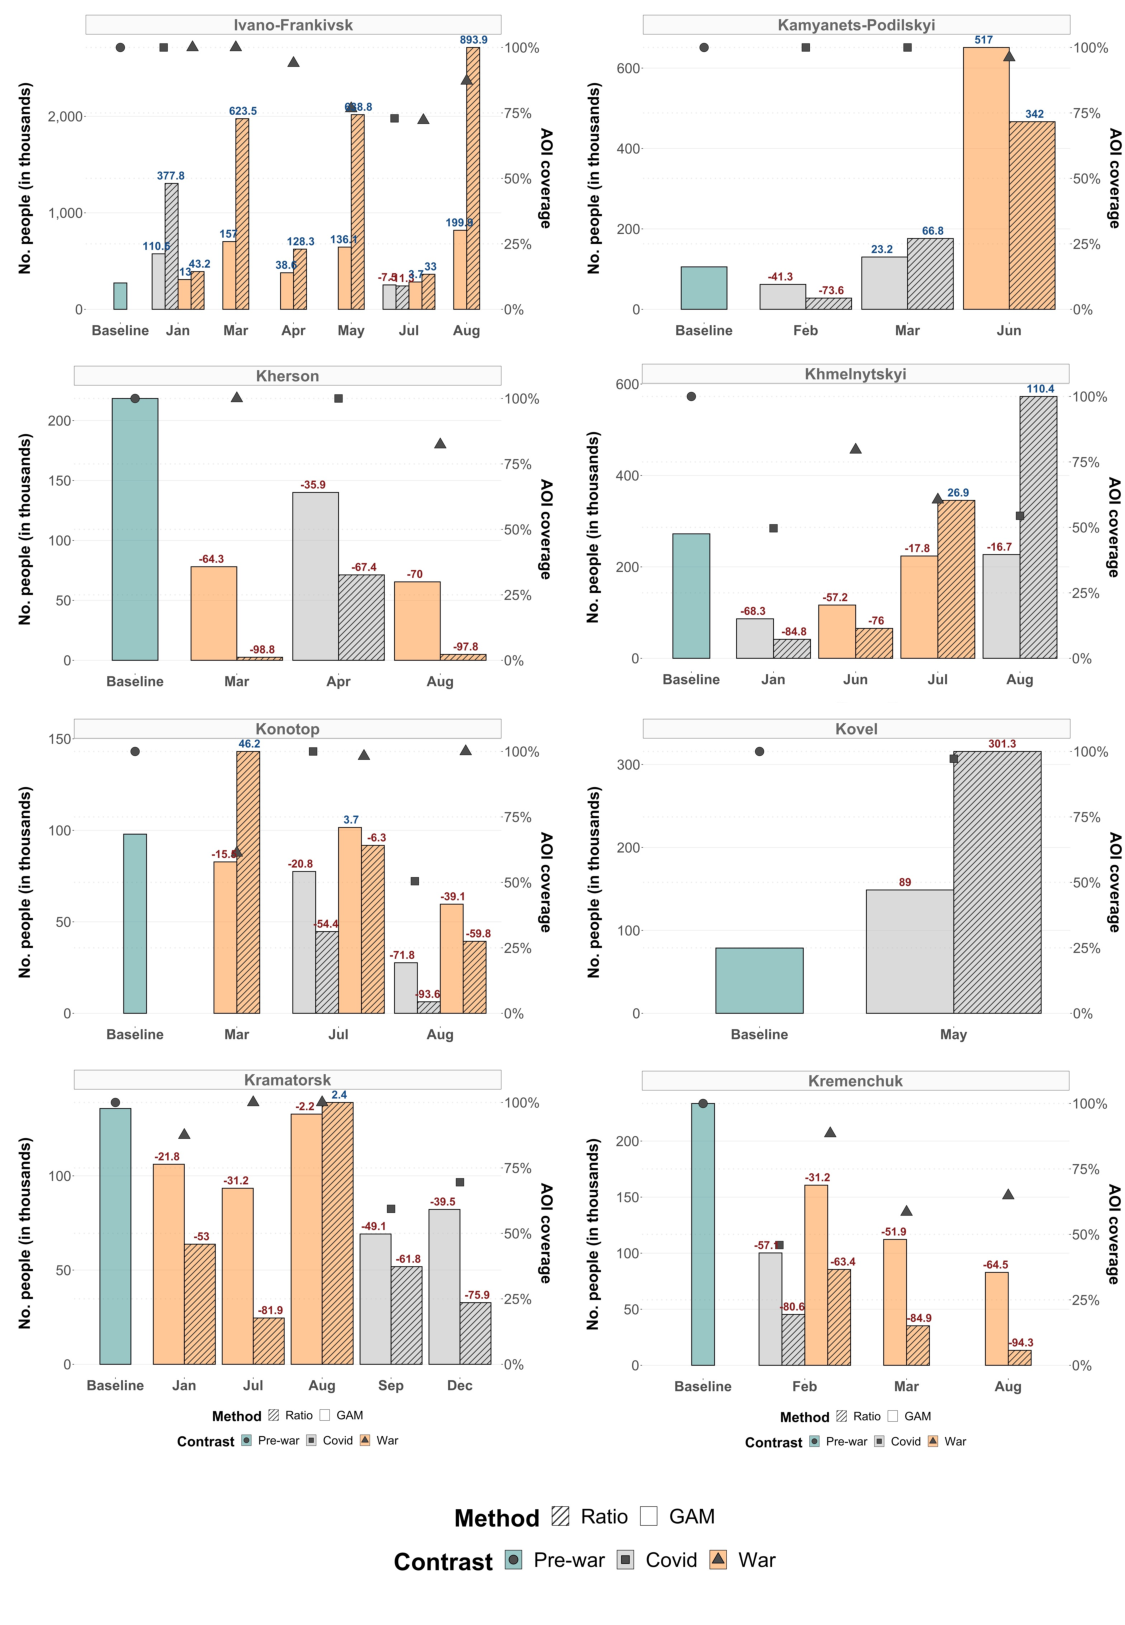
\includegraphics[scale = 0.6]{Figures/SM_IDP_pred_Fig2.pdf}
\end{center}
\caption{Cont. - Predictions of internally displaced people across three different cities in Ukraine. The turquoise bar marks the pre-War population size (2019), from which relative change in population size has been derived for the applicable months in either 2020 (first COVID-19 year, gray bars) or 2022 (War year, orange bars). Numbers on top of each bar denote the relative population change (in \%), with colors reflecting either an increase (blue) or decrease (red). Dashed and plain bars distinguish the two tested prediction methods: linear ratio (dashed) and Generalized Additive Model (GAM, plain). Moreover, the overlaid symbols, related to the secondary y-axis, depict the percentage of area covered by the satellite images underlying a given month relative to the city's area of interest (AOI).}
\label{figSM_IDP_pred_Fig2}
\end{figure}

%%% fig 3
\begin{figure}[h!]
\begin{center}
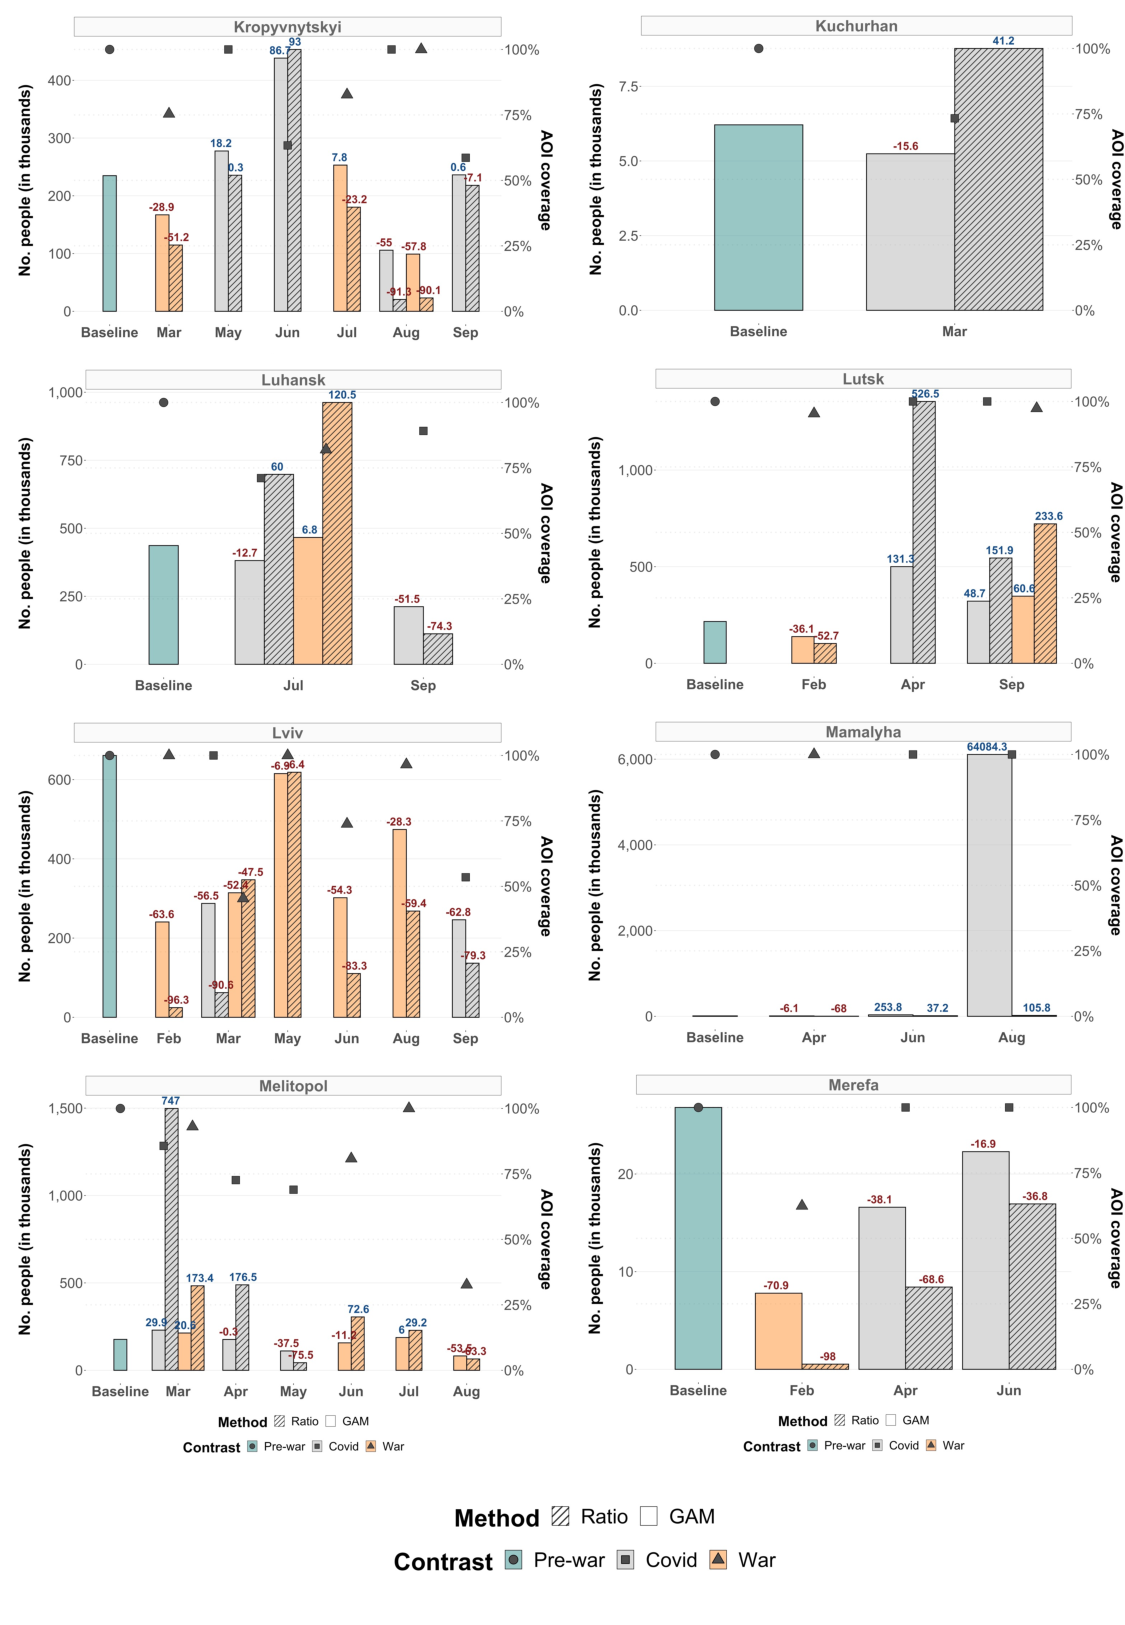
\includegraphics[scale = 0.6]{Figures/SM_IDP_pred_Fig3.pdf}
\end{center}
\caption{Cont. - Predictions of internally displaced people across three different cities in Ukraine. The turquoise bar marks the pre-War population size (2019), from which relative change in population size has been derived for the applicable months in either 2020 (first COVID-19 year, gray bars) or 2022 (War year, orange bars). Numbers on top of each bar denote the relative population change (in \%), with colors reflecting either an increase (blue) or decrease (red). Dashed and plain bars distinguish the two tested prediction methods: linear ratio (dashed) and Generalized Additive Model (GAM, plain). Moreover, the overlaid symbols, related to the secondary y-axis, depict the percentage of area covered by the satellite images underlying a given month relative to the city's area of interest (AOI).}
\label{figSM_IDP_pred_Fig3}
\end{figure}


%%% fig 4
\begin{figure}[h!]
\begin{center}
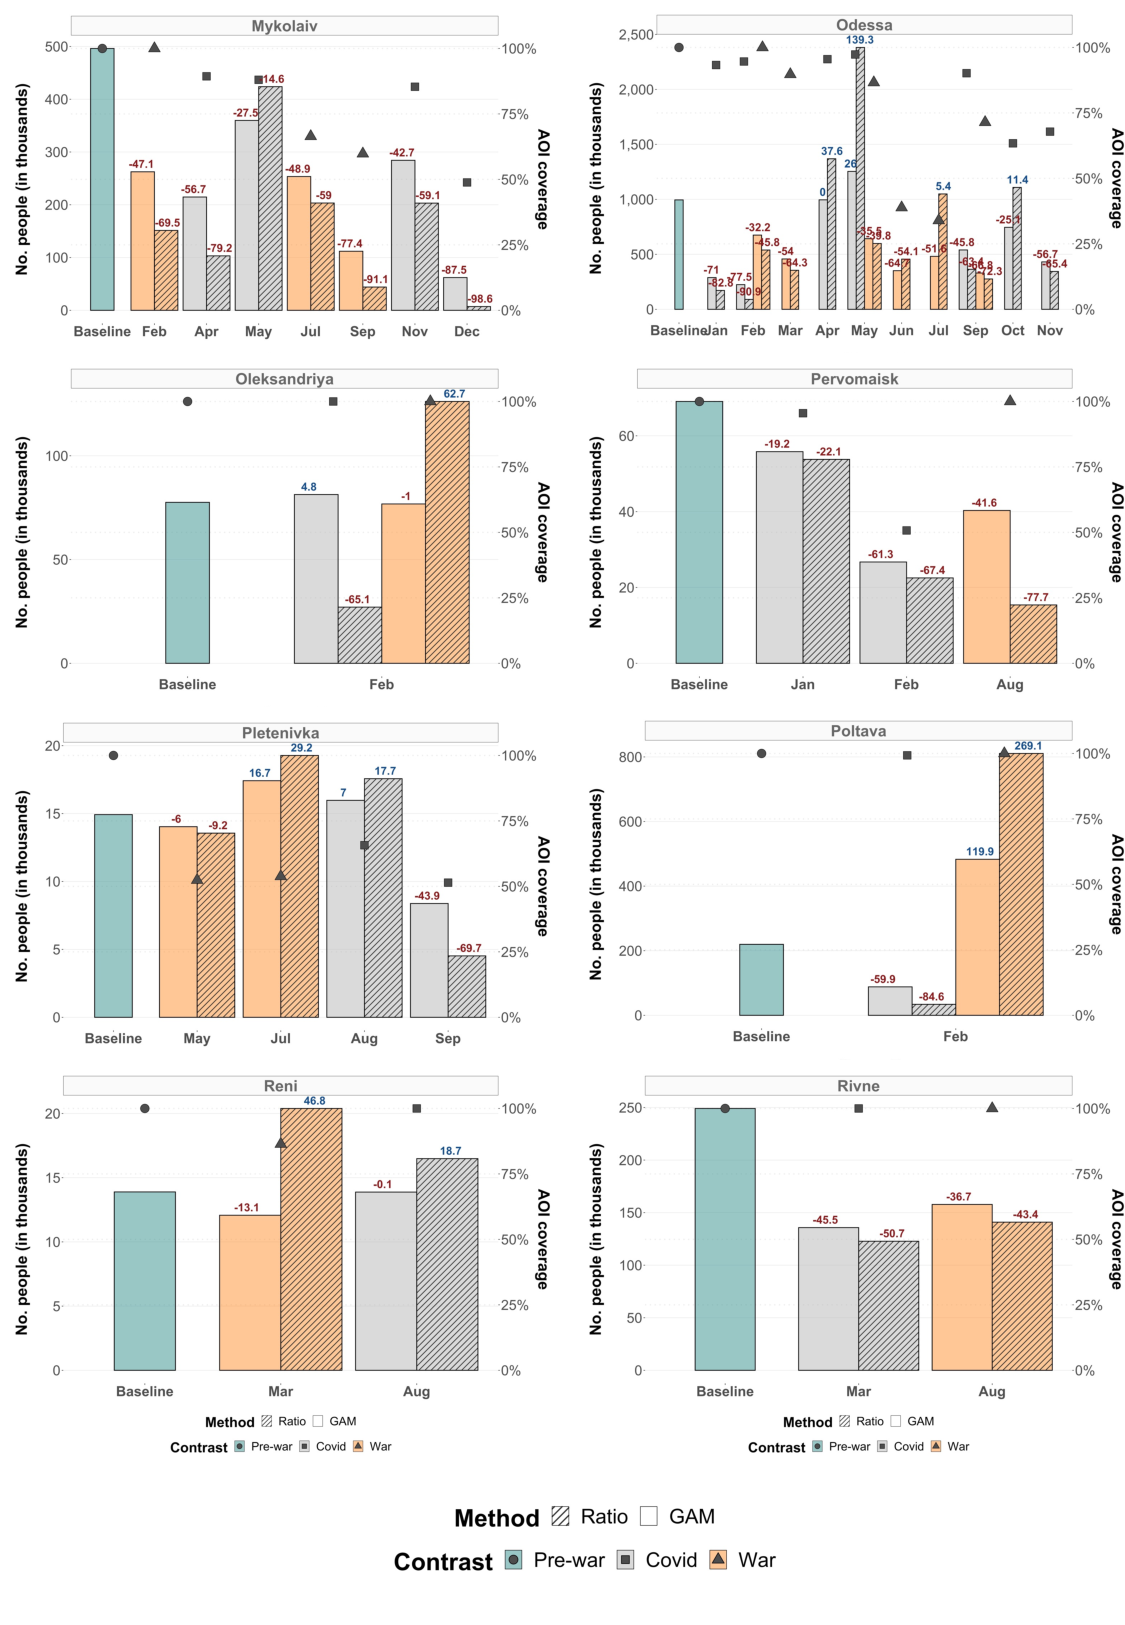
\includegraphics[scale = 0.6]{Figures/SM_IDP_pred_Fig4.pdf}
\end{center}
\caption{Cont. - Predictions of internally displaced people across three different cities in Ukraine. The turquoise bar marks the pre-War population size (2019), from which relative change in population size has been derived for the applicable months in either 2020 (first COVID-19 year, gray bars) or 2022 (War year, orange bars). Numbers on top of each bar denote the relative population change (in \%), with colors reflecting either an increase (blue) or decrease (red). Dashed and plain bars distinguish the two tested prediction methods: linear ratio (dashed) and Generalized Additive Model (GAM, plain). Moreover, the overlaid symbols, related to the secondary y-axis, depict the percentage of area covered by the satellite images underlying a given month relative to the city's area of interest (AOI).}
\label{figSM_IDP_pred_Fig4}
\end{figure}


%%% fig 5
\begin{figure}[h!]
\begin{center}
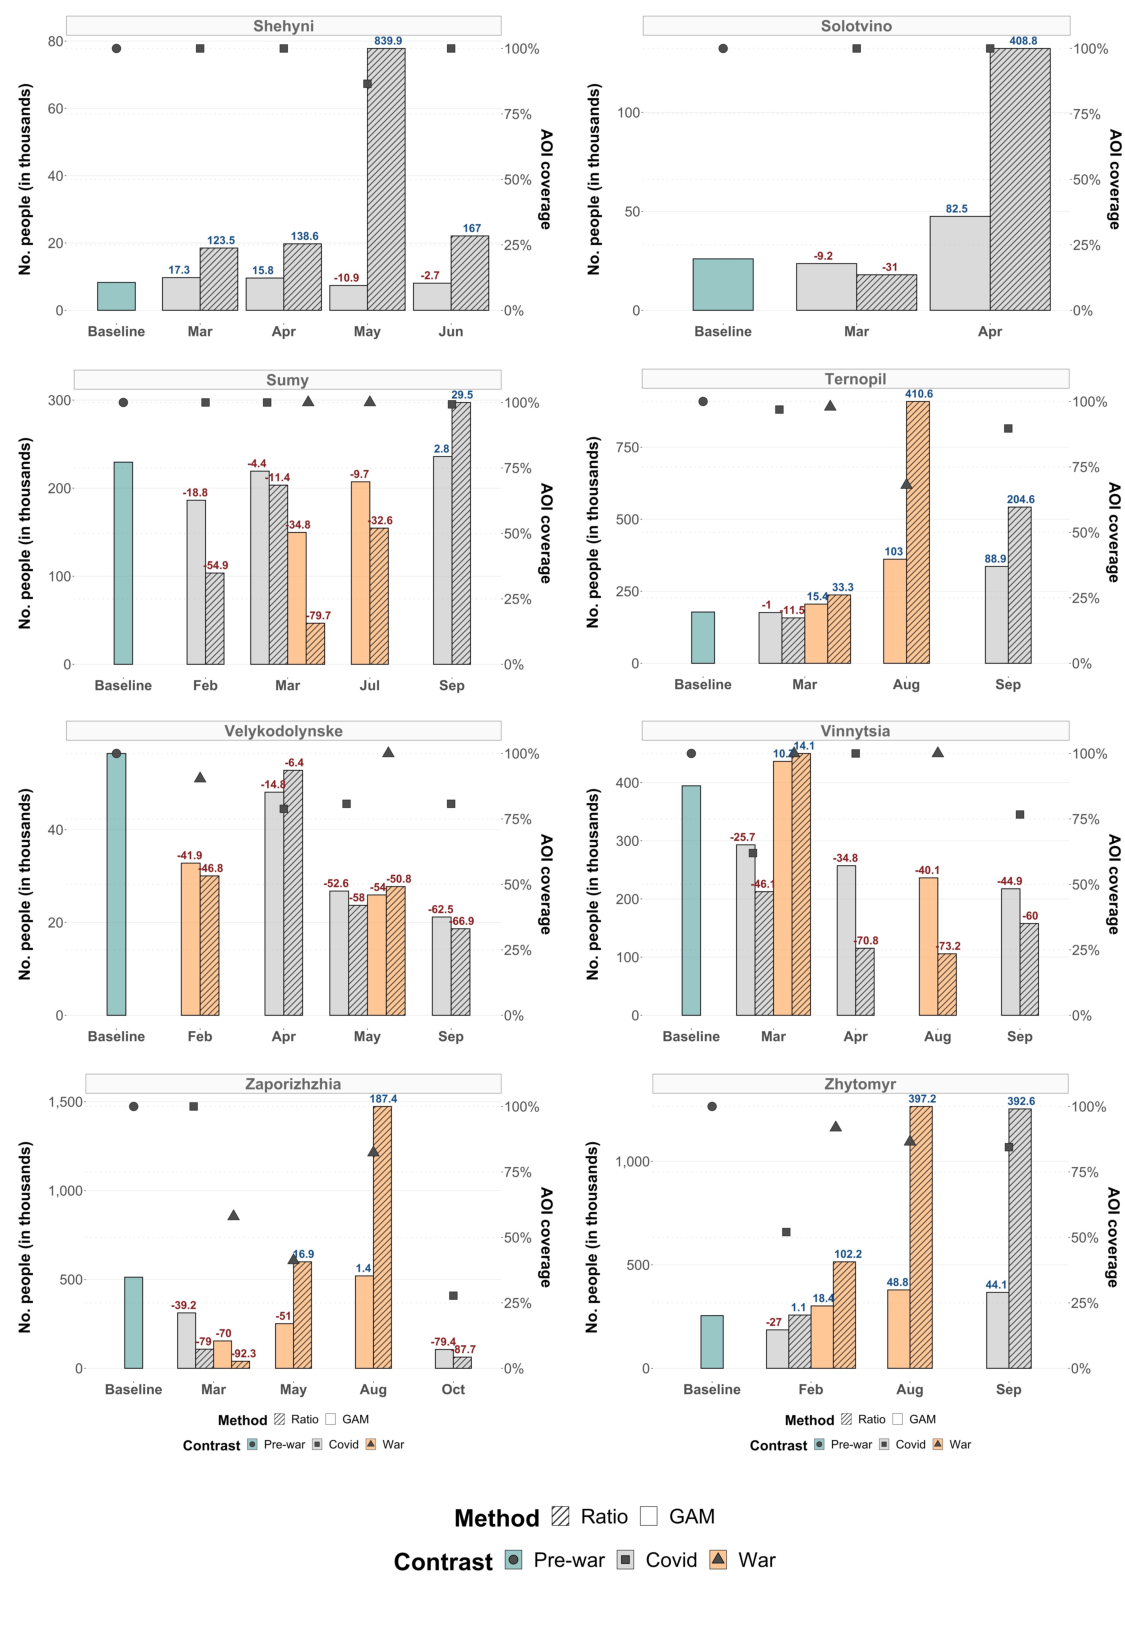
\includegraphics[scale = 0.6]{Figures/SM_IDP_pred_Fig5.pdf}
\end{center}
\caption{Cont. - Predictions of internally displaced people across three different cities in Ukraine. The turquoise bar marks the pre-War population size (2019), from which relative change in population size has been derived for the applicable months in either 2020 (first COVID-19 year, gray bars) or 2022 (War year, orange bars). Numbers on top of each bar denote the relative population change (in \%), with colors reflecting either an increase (blue) or decrease (red). Dashed and plain bars distinguish the two tested prediction methods: linear ratio (dashed) and Generalized Additive Model (GAM, plain). Moreover, the overlaid symbols, related to the secondary y-axis, depict the percentage of area covered by the satellite images underlying a given month relative to the city's area of interest (AOI).}
\label{figSM_IDP_pred_Fig5}
\end{figure}



% IDP gridded predictions - Spatial maps
%%%%%%%%%%%%%%%%%%%%%%%%%%%%%%%%%%%%%%%%%
\begin{figure}[h!]
\begin{center}
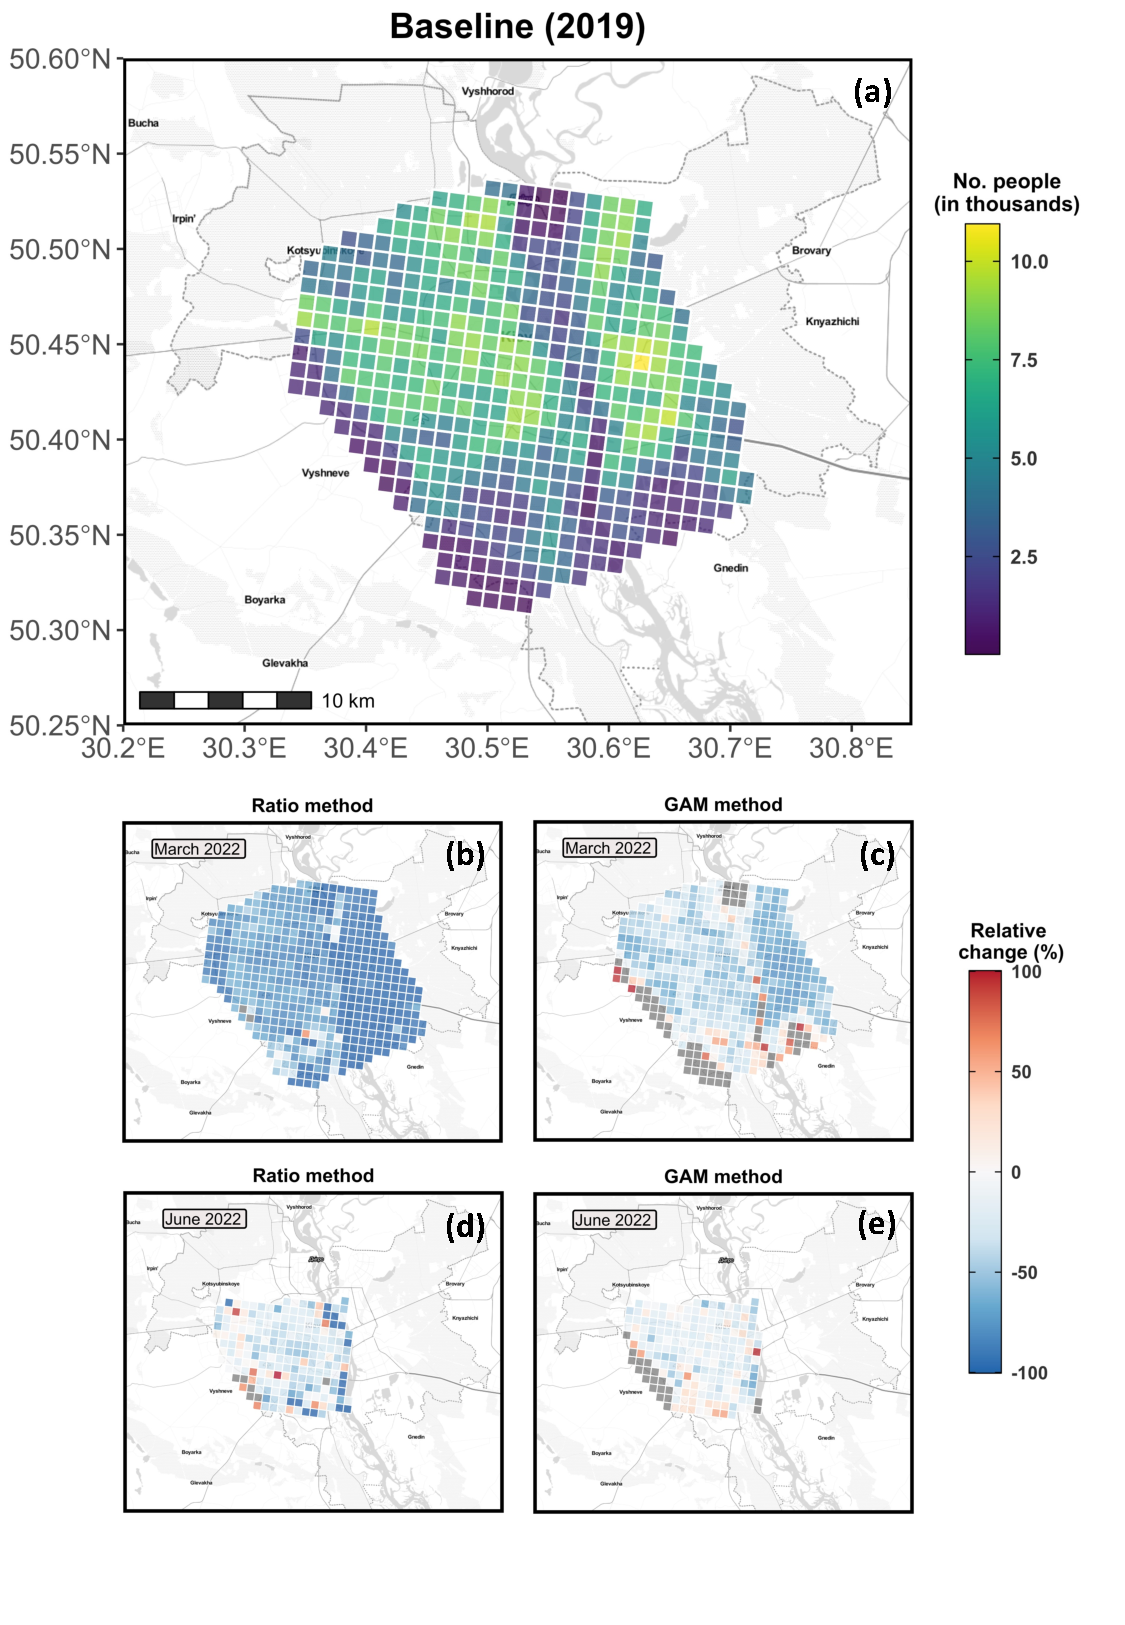
\includegraphics[scale = 0.6]{Figures/SM_gridded_predictions_relative.pdf}
\end{center}
\caption{Gridded population for Kiev city, with each grid cell measuring 1 x 1 km. The baseline population (top panel) was retrieved from WorldPop's database, whereas the population for March and June 2022 were predicted through either the Ratio (left mid and lower panels) or the Generalized Additive Model (GAM, right mid and lower panels) method. Color scale in the four lower panels reflect the percentage change of the popoulation in 2022 relative to 2019. Gray colored grid cell represent cases where the predicted population exceeded the limits of the color range, and were thus omitted to maintain a discernible color scale.}
\label{figSM_gridded_pred}
\end{figure}



% Visual evaluation of GAM fit
%%%%%%%%%%%%%%%%%%%%%%%%%%%%%%%%%%%%%%%%%
\begin{figure}[h!]
\begin{center}
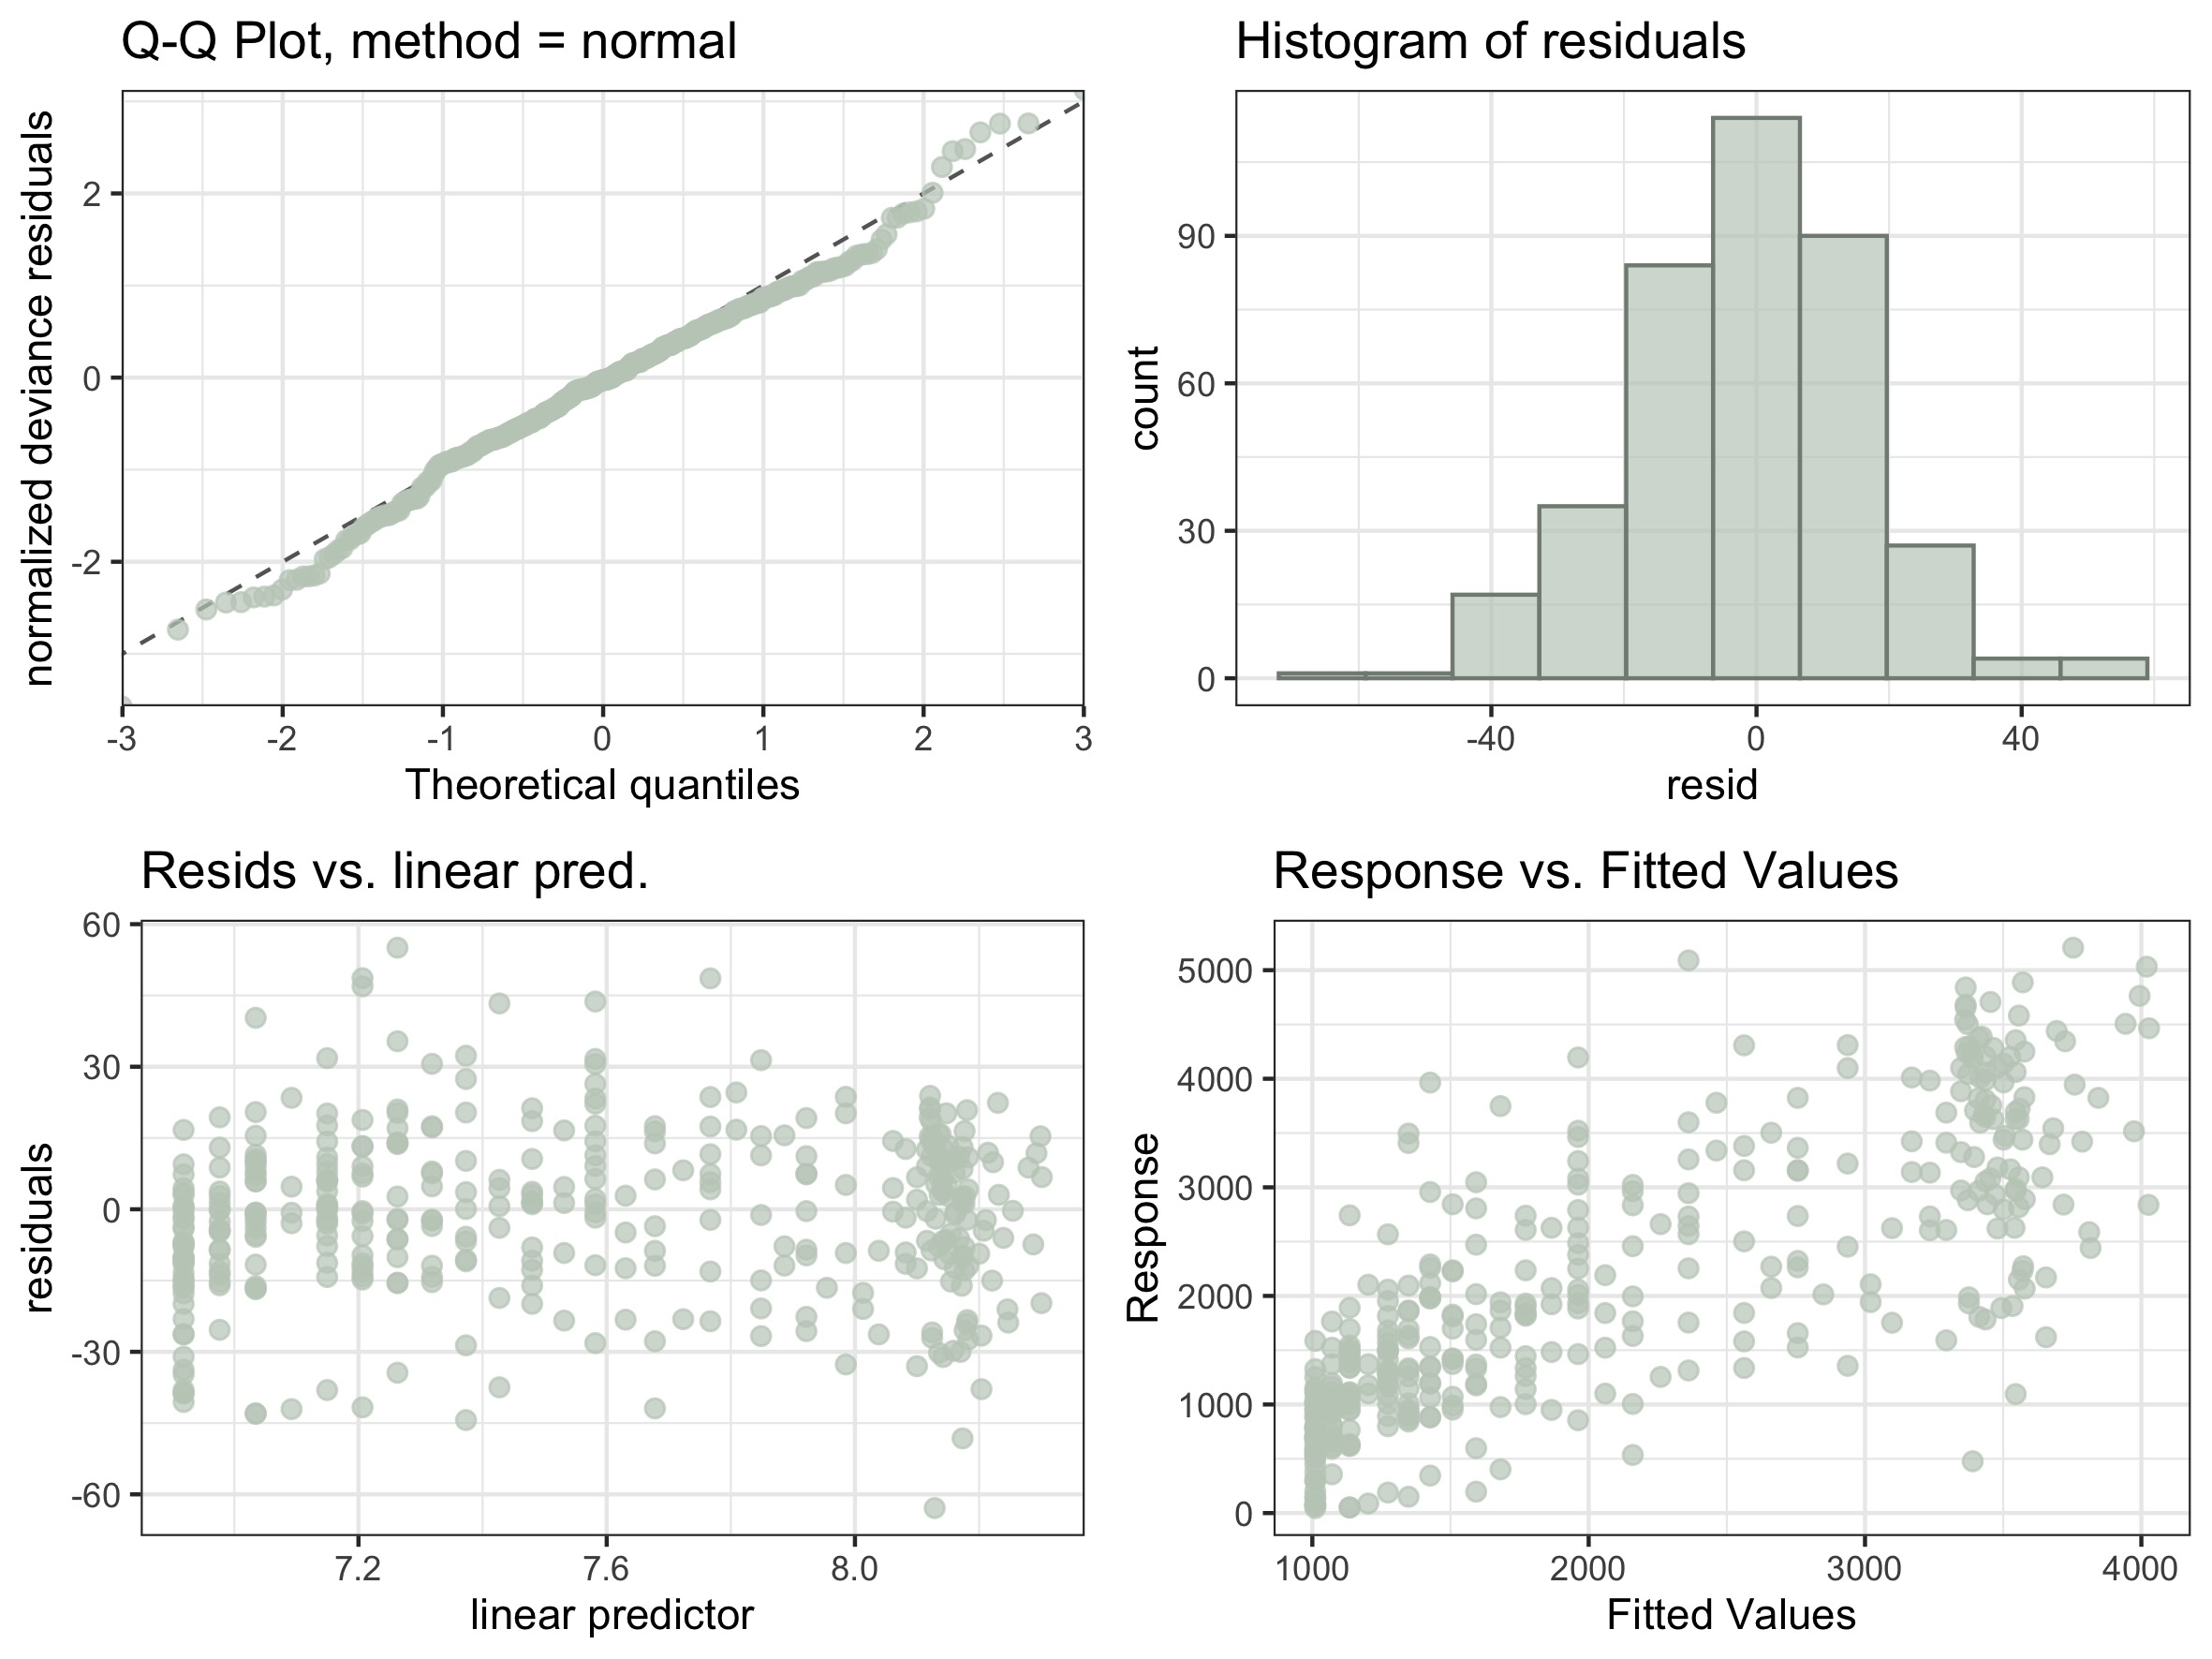
\includegraphics[width = \textwidth]{Figures/SM_GAMfit.jpg}
\end{center}
\caption{Visual inspection of the Generalized Additive's Model assumption for the city of Donetsk. Upper panels shows the residuals' normality through the Q-Q plot and histogram, whereas residual's homogeneity is confirmed in the lower left panel (no trend should be detected between residuals and the estimated values). The predictive quality of the model can be also traced in the lower right panel, where the observed values should be linearly and tightly correlated with the values estimated by the model. Results for the remaining cities can be accessed on the first author's GitHub repository (\url{https://github.com/mcruf/IDP_UKR}).}
\label{figSM_GAMfit}
\end{figure}






\end{appendices}

%%===========================================================================================%%
%% If you are submitting to one of the Nature Portfolio journals, using the eJP submission   %%
%% system, please include the references within the manuscript file itself. You may do this  %%
%% by copying the reference list from your .bbl file, paste it into the main manuscript .tex %%
%% file, and delete the associated \verb+\bibliography+ commands.                            %%
%%===========================================================================================%%

\clearpage
%\bibliographystyle{sn-nature} %
\bibliography{sn-bibliography}% common bib file
%% if required, the content of .bbl file can be included here once bbl is generated
%%\input sn-article.bbl


\


\end{document}
